%\documentclass[12pt]{book}
\documentclass[12pt]{report}
\usepackage{Template/suthesis-2e}
\usepackage{geometry}        
\geometry{letterpaper}    
\usepackage[parfill]{parskip}  
\usepackage{deluxetable}
\usepackage{graphicx}
\usepackage{amssymb}
\usepackage{epstopdf}
\usepackage{amsmath}
\usepackage{multirow}
\usepackage{caption}
\usepackage{subcaption}
\usepackage{multicol}
\usepackage{array}
\usepackage{amsmath}
\usepackage{afterpage}
\usepackage{longtable}
\usepackage{booktabs}
\usepackage{wrapfig}
\usepackage{float}
\usepackage{subcaption}

\usepackage[colorlinks=true, pdfstartview=FitV, linkcolor=blue 
            citecolor=blue, urlcolor=blue]{hyperref}
\usepackage{bm}
\usepackage{slashed}
\usepackage{mathrsfs}
\hypersetup{
  colorlinks=true,
  linkcolor=red,
  citecolor=red,
  urlcolor=blue
}
\DeclareGraphicsRule{.tif}{png}{.png}{`convert #1 `dirname #1`/`basename #1 .tif`.png}

%\usepackage[colorlinks=true, pdfstartview=FitV, linkcolor=blue 
 %           citecolor=blue, urlcolor=blue]{hyperref}

%\includeonly{Chapter1}



%\newtheorem{theorem}{Theorem}
%\newtheorem{corollary}[theorem]{Corollary}
%\newtheorem{definition}{Definition}
%\newtheorem{lemma}{Lemma}
%\newtheorem{exercise}{Exercise}
%\newtheorem{remark}{Remark}
%\newtheorem{example}{Example}
%\newtheorem{warning}{Warning}

\def\grad{ \mbox{grad}}
\def\curl{ \mbox{curl}}
\def\div{ \mbox{div}}
\def\U{\ensuremath {\cal U}}
\def\S{\ensuremath {\cal S}}
\def\V{\ensuremath {\cal V}}
\def\R{\ensuremath {\cal R}}
\def\tr{\ensuremath {\mbox{tr}}}
\RequirePackage{xspace}
%\RequirePackage{color}

%Units
%This is defined in the atlas style
%\def\pb {\ensuremath{{\rm \,pb^{-1}}}\xspace}

%Abbrev
\def\Geant {GEANT\xspace}
\def\mbb {\ensuremath{m_{bb}}}
\def\pt {\ensuremath{p_{\mathrm{T}}}\xspace}
\def\j145{EF\_2b35\_loose\_j145\_2j35\_a4tchad\xspace}
\def\Et {\ensuremath{E_{\mathrm{T}}}\xspace}
\def\sob {\ensuremath{S/\sqrt{S+B}}\xspace}
\def\met {\mbox{${\hbox{$E$\kern-0.63em\lower-.18ex\hbox{/}}}_{T}$}}

%Analysis Numbers
\def\MULumi {4.5~\ifb\xspace}
\def\MUObsEvts {3.0\xspace}
%\def\MUExpEvts {\ensuremath{0.82 \pm 0.26}\xspace}
\def\MUExpProbEvtsReco{\ensuremath{12.59 \pm 5.00}\xspace}
\def\MUExpProbEvts{\ensuremath{2.20 \pm 0.91}\xspace}
\def\MUExpABCDEvts{\ensuremath{0.48}\xspace}
\def\MUIsoCut {0.3\xspace}
\def\MUPtCut {11.0\xspace}

\def\EMLumi {XX~\ifb\xspace}

\def\atlas {ATLAS}




% ------------------- Title and Author -----------------------------

\begin{document}
	\title{A Search for Non-Standard Model Higgs Bosons Produced in Association with $b$-Quarks at the ATLAS Experiment}
	\author{Caitlin Malone}
	\dept{Physics}
    \principaladviser{Su Dong}
%    \firstreader{Patricia Burchat}
%    \secondreader{Lance Dixon}

\beforepreface
\prefacesection{Abstract}
With the discovery of a Standard-Model-like Higgs boson at the LHC 
in 2012, the particle content of the Standard Model has been fully verified experimentally,
and the focus turns even more fully to searches for physics beyond the Standard Model.  
One interesting class of theories, supersymmetry, predicts (at least) 4 additional 
Higgs bosons.  This is a search for two of those SUSY Higgs particles, 
$A^0$ and $H^0$, in production states including additional $b$-quarks and in final 
states where $A^0$ and $H^0$ are decaying to a $b\bar{b}$ final state.  
Using data-driven estimations to understand and model the large multi-$b$-quark 
QCD backgrounds at the LHC, we set limits on the production cross section times 
$b\bar{b}$ branching ratio of $A^0$ and $H^0$ in the range 450 GeV $<m_{A^0}<$ 800 GeV.  
This is the first resonance search in this final state at ATLAS, and the 
highest-mass search for $A^0$ and $H^0$ decaying to $b\bar{b}$ that has yet been performed.
\prefacesection{Acknowledgements}
This section to be added
\afterpreface

%\frontmatter
%\maketitle

%\tableofcontents
%\listoffigures
%\listoftables


% Activate the following line by filling in the right side. If for example the name of the root file is Main.tex, write
% "...root = Main.tex" if the chapter file is in the same directory, and "...root = ../Main.tex" if the chapter is in a subdirectory.
 
%...root =  ../thesis.tex

\chapter[Theory of Higgs Physics]{Higgs Boson Physics, in the Standard Model and in Supersymmetry}
\label{chapter:Theory}



\section{Introduction}
The goal of particle physics is to understand the fundamental particles of the universe and 
their interactions. It's a field that is simultaneously impressively advanced but 
with tantalizingly unresolved aspects; in general, progress in the field is a team 
effort between theorists who propose new physics possibilities and the experimentalists who build 
large accelerators and detectors and analyze the resulting data for hints of new physics.  The project of this thesis is 
an experimental search for two new particles, the Supersymmetric Higgs bosons $H$ 
and $A$, at the ATLAS detector at the Large Hadron Collider.

In order to understand the relevance of this search, and how it is performed, 
we must first understand the Standard Model of particle physics, including the Higgs mechanism, 
and its extensions in Supersymmetry.  The Standard Model is the outcome of decades of 
experimental and theoretical work in particle physics; it describes all the known particles and 
their interactions.  It is one of the most thoroughly tested theories in all of 
science, and it has yet to give a prediction that is not experimentally borne 
out--an impressive feat.  At the same time, there are known blind 
spots in the Standard Model, since it does not include gravity, explain dark 
matter or dark energy, or account for the origin of the baryon asymmetry of the universe
\footnote{in other words, why the universe is made of matter instead of antimatter}.   The shortcomings of the 
Standard Model motivate searches for Beyond-Standard-Model (BSM) physics, including Supersymmetry.  


\section{The Standard Model}
The Standard Model of particle physics was painstakingly constructed over the 20th century and stands 
as one of the most thoroughly-verified theories in science.  The Standard Model 
(SM) is a quantum field theory that incorporates two different types of matter 
particles, the quarks and the leptons, as well as three fundamental forces and 
their corresponding particles.  However, as we will see, it has several notable 
shortcomings that attract considerable attention from both theorists and experimentalists.  

\subsection{Quarks and Leptons}
The quarks and the leptons are perhaps the most familiar subatomic particles, as they 
are the particles that make up matter.  For example, a hydrogen atom is 
composed of a proton (three quarks) and an electron (a lepton).  
There are six quarks total, three ``up-type'' with an electric 
charge of +2/3 and three ``down-type'' with charge 
of -1/3.  There are also three leptons, which are electrically 
charged and massive (the electron, muon and tau), and three neutrinos, 
which are electrically neutral and nearly massless (the electron, muon and tau neutrinos).  
We can classify the quarks and leptons according to ``generation'', where each generation 
is composed of one up-type quark, one down-type quark, 
one lepton, and one neutrino.  The quarks and leptons are summarized in Table \ref{tab:QLTable}.

\begin{table}
	\caption{A summary of the fermions.  In the ``SM interactions'' column, 
    S stands for the strong nuclear force, W is the weak nuclear force, 
    and EM is the electromagnetic force.  As is customary in particle physics, 
    the mass is measured in units of energy divided by the speed of light squared 
    (since $E=mc^2$), although in practice the $c^2$ is often 
    dropped and masses expressed simply in units of energy, typically electron-volts (eV) or multiples thereof. 	\label{tab:QLTable}}
	\begin{tabular}{| c || c | c | c | p{2cm} |}
%		\multicolumn{3}{c}{Quarks} \\
		\hline
		Generation &  Flavor & Electric Charge & Mass (MeV/$c^2$) & SM Interactions\\
		\hline
		\multirow{4}{*}{1} & up quark \it{(u)} & +2/3 & 2.3 & S, W, EM\\
		    & down quark \it{(d)} & -1/3 & 4.8 & S, W, EM\\
		    & electron \it{(e)}& -1 & 0.511 & W, EM \\
		    & electron neutrino \it{($\nu_{e}$)} & 0 & $<$2.2$\times 10^{-6}$ & W\\
		\hline
		\multirow{2}{*}{2} & charm quark \it{(c)} & +2/3 & 1290 &  S, W, EM \\
		    & strange quark \it{(s)} & -1/3 & 95 & S, W, EM \\
		    & muon \it{($\mu$)} & -1& 105.7 & W, EM \\
		    & muon neutrino \it{($\nu_{\mu}$)} & 0 & $<$0.170 & W \\
		\hline 
		\multirow{2}{*}{3} & top quark \it{(t)} & +2/3 & 173,340 & S, W, EM \\
		    & bottom quark \it{(b)} & -1/3  & 4180 & S, W, EM \\ 
		    & tau \it{($\tau$)} & -1 & 1776 & W, EM\\
		    & tau neutrino \it{($\nu_{\tau}$)} & 0 & $<$15.5 & W\\		    
		\hline
	\end{tabular}
\end{table}


\begin{table}
	\caption{The bosons of the Standard Model: their masses and interactions.   
    The interactions between the Higgs field and the fermions are not usually characterized as 
    a force, per se, but rather it is the interaction between the 
    Higgs field and the W boson, Z boson, and fermions that gives mass to the particles.  \label{tab:boson_table}}
    \center
	\begin{tabular}{| c || c | c |}
	\hline
	Particle & Associated Force & Mass \\
	\hline
	gluon & strong & massless \\
	photon & electromagnetic & massless \\
	W$^\pm$ & weak & 80.4 GeV \\
	Z & weak & 91.2 GeV \\ 
	Higgs boson & Higgs field & 126 GeV \\
	\hline
	\end{tabular}
\end{table}


All of the quarks and leptons are fermions, meaning they have half-integer spin.

\subsection{Bosons and Forces}

The forces between fermions are carried by bosons, which are integer spin particles.  
There are three forces described in the Standard Model: electromagnetic, weak, and 
strong.  The electromagnetic force is carried by the photon and describes, for example, 
electric forces between particles.  Photons are massless and as a result, the electromagnetic 
field can extend infinitely far.  The weak force is carried by W$^+$, 
W$^-$ and Z$^0$ bosons.  These particles are massive, which 
means that they are limited in how far they can travel and thus the weak 
force is confined to distance scales approximately the size of an atomic nucleus.  The 
weak force is involved when one type of fermion changes into another type of fermion, 
for example, when a neutron decays or a nucleus fissions.  The strong force 
is carried by gluons, which are massless but because of confinement, the strong 
force is restricted to the nuclear scale.  The strong force is responsible for holding 
quarks together into protons, neutrons and other hadrons. Last, there is the 
gravitational force, which we will neglect as it is many orders of magnitude weaker 
than the other forces under discussion.

The electromagnetic and weak forces, as it turns out, can be unified into a single ``electroweak'' force, as discovered in the middle part of the 20th century \cite{Weinberg}.  The vector bosons acquire mass, which is known as electroweak symmetry breaking, via the Higgs mechanism \cite{Higgs-1} \cite{Englert_Brout} \cite{Guralnik_Hagen_Kibble}.  The Higgs mechanism, and the particle which conveys the Higgs field (the Higgs boson), are explained in more detail in further sections.  Further unification of forces, between the electroweak and strong forces, remains an unfinished project in physics but a topic of much research.  

\section{Electroweak Symmetry Breaking and the Higgs Mechanism in the Standard Model}
The Standard Model is defined by its Lagrangian, which is a mathematical formula that 
encodes all the Standard Model particles and their interactions.  The SM Lagrangian was built 
piece by piece over many decades, starting with classical field theory and later being 
generalized to account for relativity, electromagnetism, the strong and weak forces, and 
the unification of the weak and EM forces (this is not an exhaustive list 
of the features of the SM Lagrangian, of course).  

Different terms in the SM Lagrangian account for different types of particles.  The fermions, 
which have spin 1/2, are governed by the Dirac Lagrangian:

\begin{equation}
\mathscr{L}= i bar{\psi} \gamma^\mu \partial_\mu \psi -m \bar{\psi}\psi \footnote{we use the physics notation custom of $\hbar=c=$1 in this section}
\end{equation}

(Similarly, the Klein-Gordon Lagrangian is used for spin-0 particles, 
and the Proca Lagrangian for spin-1.)  When the Dirac Lagrangian is plugged 
into the Euler-Lagrange equations, the equation that results is a quantum field 
theory equation describing a particle of mass $m$ and spin $\frac{1}{2}$.  

One problem with simply using the Dirac Lagrangian as-is arises because 
the Dirac Lagrangian is not invariant under local phase transformations.  In other 
words, if the field $\psi$ is multiplied by an exponential term with 
a space-dependent (``local'') phase, $\psi \rightarrow e^{iq\theta(x)} \psi$, 
then plugging the new $\psi$ into the Euler-Lagrange equations will result 
in an extra term because of the derivative of $\theta(x)$.  This 
is what we mean by saying that as it is written, the Dirac Lagrangian 
is not invariant under local phase transformations.  The fix for this problem is to 
replace the ordinary derivative with the covariant derivative:

\begin{equation}
\mathscr{D}_\mu \equiv \partial_\mu - iqA_\mu
\end{equation}

The second term in the covariant derivative cancels the extra term from the derivative of 
$\theta(x)$, and local phase invariance is reinstated.  However, when 
we added the second term, we added in a new field $A_\mu$ 
which must also show up in the Lagrangian but be massless ($m_A$=0) 
in order to preserve the local gauge invariance that we have so carefully constructed.  
The trouble here is that, when we think about this formalism being used to 
describe the weak force, the corresponding $W$ and $Z$ bosons 
are definitely \textit{not} massless.  What we need is a modification 
to this procedure that will leave us with at least two massive degrees of freedom, 
which we can interpret as the $W$ and $Z$, and no massless particle corresponding to $A_\mu$.

Let's now consider what happens when the Lagrangian has a slightly different functional 
form: instead of a quadratic term $-mc^2\bar{\psi}\psi$, 
it's perfectly valid to have a quartic term also: $-\mu^2\psi^2+\lambda^2 \psi^4$.  
In this case, however, ground state of the field $\psi$ does 
not occur when $\psi=0$, but rather when $\psi$ takes 
on a value of $\psi = \pm \mu^2/\lambda$.  
There is a symmetry as to whether $\psi$ takes on the positive or 
negative solution to the equation; the fact that the system must pick one solution 
or the other means that it undergoes \textit{spontaneous symmetry breaking}.

The Higgs mechanism is the powerful combination of local gauge invariance and spontaneous symmetry 
breaking, which achieves our goal of getting rid of the massless $A_\mu$ 
term while allowing $W$ and $Z$ to be massive.  The 
field $\psi$ is a complex field, with both a real and imaginary 
part $\psi=\psi_1+i\psi_2$, which we can make locally invariant 
by the same trick as before (replace the derivative with the covariant derivative, 
and add in a new field $A_\mu$).  If, however, 
the Lagrangian has a form that allows for spontaneous symmetry breaking, the field 
$\psi$ can undergo a change of variables $\eta\equiv \psi_1 - \mu/\lambda$, 
$\xi\equiv \psi_2$ and the Lagrangian can be rewritten 
in a way that the massless gauge field $A_\mu$ has now 
acquired a mass.  The massless particle we first encountered when trying to write a 
locally-invariant Lagrangian is represented by the $\xi$ term.  A transformation 
of the $\psi$ field $\psi \rightarrow \psi' = (cos\theta + i sin\theta)(\psi_1+i\psi_2)$, 
with $\theta=tan^{-1}(\frac{\psi_2}{\psi_1})$ 
makes $\psi_2'=0$, which gets rid of the massless particle 
that was troubling us before.  If we generalize this analysis to a  complex scalar 
doublet, which has four degrees of freedom (this example had 2), we 
will have 4 massive particles.  Three of these are the gauge bosons, 
$W^\pm$ and $Z$; the fourth is a new massive scalar particle which we call the Higgs boson.



 
 
 
\section{Supersymmetry}

\begin{centering}
    \begin{figure} \center
    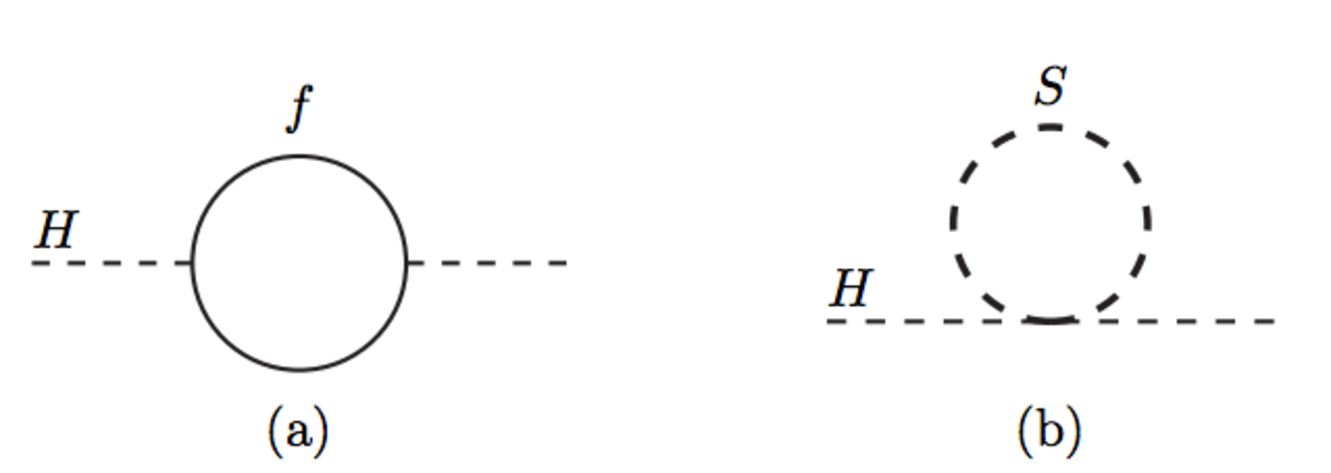
\includegraphics[width=0.6\textwidth]{Theory/FeynmanDiagrams/Higgs_mass_corrections.pdf}
    \caption{The radiative corrections to the Higgs mass can be seen
    in these Feynman diagrams, with a fermionic correction to the mass shown on the left and 
    the correction from a scalar particle on the right.  One problem with the bare Standard Model
    is that corrections such as these need to cancel to an incredible
    degree of precision, one part in $10^{30}$, to allow the Higgs to have a mass of 126 GeV. \cite{martin}
    \label{fig:higgs_mass_corrections}}
    \end{figure}
\end{centering}

Despite its robustness in the face of experimental scrutiny, the Standard Model has several 
important shortcomings.  One of the most important is the hierarchy problem, which refers 
to the divergence of the Higgs mass via contributions from quantum loop corrections.
On one hand, it is true at tree level (and now experimentally verified) that the Higgs 
mass is of the same order of magnitude as the masses of the electroweak bosons.  
On the other hand, the Higgs mass can receive large corrections via its coupling
to fermion-antifermion 
pairs\footnote{most notably the top quark, since the size of the correction is proportional
to the mass of the particle in the loop correction} and W and Z bosons, and
even self-coupling of the Higgs to itself, 
all of which introduce correction terms to the Higgs mass.  For example, the 
diagram shown in Figure~\ref{fig:higgs_mass_corrections} (a) 
contributes the following correction term to the mass:

\begin{equation}
	\delta m_H^2 = - \frac{|\lambda_f |^2}{8\pi^2}[\Lambda_{UV}^2+\ldots]
\end{equation}

$\Lambda_{UV}$ is the ultraviolet cutoff scale, the energy at which 
the Standard Model breaks down and new physics must enter the picture, and 
$\lambda_f$ is the Yukawa coupling to the fermion in question.  The 
exact value of $\Lambda_{UV}$ is not known, but a reasonable 
a priori guess would be the Planck scale, about $10^{19}$ 
GeV.  However, since the experimentally measured mass of the Higgs is about 126 
GeV, there needs to be fine-tuning on the scale of one part in  
$10^{30}$ GeV for the numbers to come out correctly.

Supersymmetry solves this problem by introducing a mirror set of particles to the Standard Model 
particles, where each SM boson has a corresponding supersymmetric fermion and each SM fermion 
has a SUSY boson.  These SUSY particles would also couple to the Higgs, 
and introduce additional terms to the mass, namely

\begin{equation}
	\delta m_H^2 = \frac{|\lambda_s |^2}{16\pi^2}[\Lambda_{UV}^2-2m_s^2ln(\Lambda_{UV}/m_s)+\ldots]
\end{equation}

The ultraviolet cutoff $\Lambda_{UV}$ enters again here, this time with 
the opposite sign, so that the two terms end up largely canceling when the Higgs mass is computed. 
If the scalar particle in Figure 1.1(b) is the superpartner of the fermion in 1.1(a),
the Yukawa couplings $\lambda_s$ and $\lambda_f$ could quite elegantly have very 
similar values and the large correction terms cancel, leaving us with a Higgs mass
much closer to the value seen experimentally. 

Taken at face value, SUSY requires that the supersymmetric partners have the same masses 
as their SM counterparts.  If this were the case, though, we would 
have seen the SUSY particles already--they would have been produced at experiments
at the Tevatron and LEP, to say nothing of the LHC.
The lack of SUSY particles with the same masses as their SM counterparts 
leads us to say that supersymmetry is ``broken'' (in the sense 
that is is not a symmetry of the vacuum, not in the sense that 
it does not hold theoretically).  When we consider broken supersymmetric theories, the 
masses of the SUSY particles can become large, and indeed the mass limits for 
SUSY particles now require that most of them are at least several hundred GeV, up 
to several TeV.  One problem with this trend is that the supersymmetric solution to 
the hierarchy problem assumes SUSY partners that are light, less than a TeV or 
so, so that the SUSY contributions to the Higgs mass are roughly the same 
size as the SM contributions.  As direct and indirect searches exclude much of the 
phase space below a few TeV, it becomes harder to find SUSY scenarios that 
elegantly solve the hierarchy problem and SUSY becomes less appealing in that sense. 

SUSY has additional motivations, however.  Another appealing feature of SUSY is that it 
changes the logartihmic evolution of the coupling constants of the three SM forces.  At very high energies the 
coupling constants come close to the same value, but do not quite match up, 
a theoretically unsatisfying fact that SUSY addresses.  When SUSY enters the picture, the 
running values of the coupling constants change such that they unify at a high energy scale.

\begin{figure}
    \center
	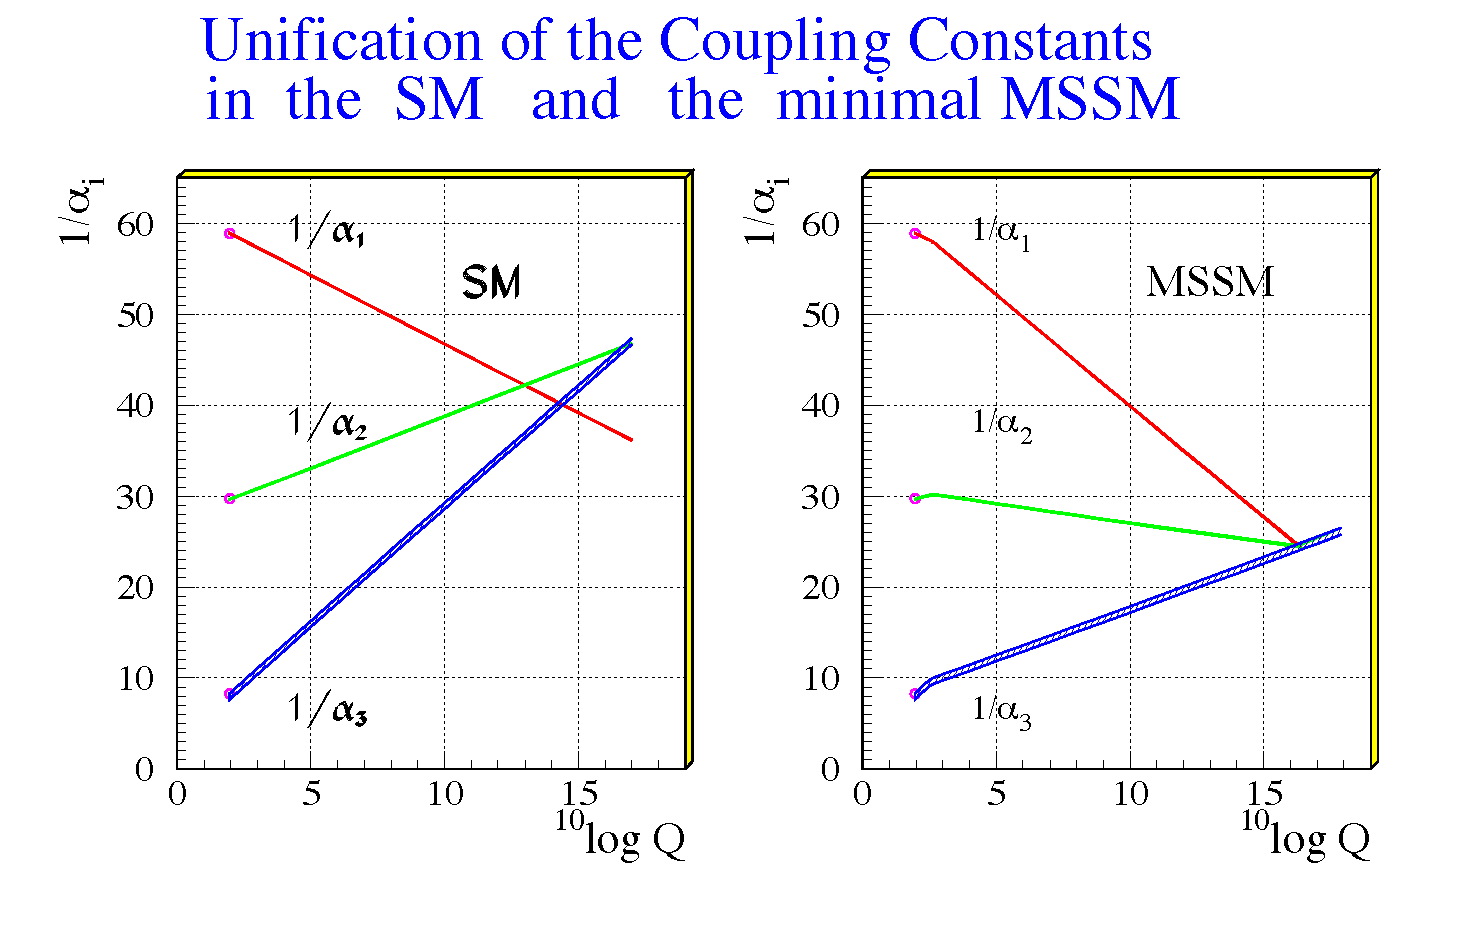
\includegraphics[width=0.8\textwidth,angle=270]{Theory/figures/kazakov_coupling.pdf}
    \caption{The coupling constants for the three fundamental forces of the Standard Model, as a 
    function of energy.  On the left, the coupling constants almost unify 
    (but don't quite meet) in the SM-only framework, 
    whereas on the right there is unification when SUSY effects are allowed to 
    enter the picture at around 1 TeV\cite{Kazakov}. }
	\label{fig:couplings}
\end{figure}


A third appealing feature of SUSY is that it provides a natural candidate for dark 
matter.  From studies of galactic rotational curves, and other astrophysical investigations, it 
seems clear that there is a significant amount of matter (``dark matter'') floating 
around the galaxy that does not interact via the electromagnetic or strong nuclear forces, 
but does interact gravitationally (it is not known whether it interacts via the weak 
nuclear force; a number of experiments are attempting to detect it via the weak 
force but so far have not produced clear and unequivocal evidence).  Among the supersymmetric 
particles would be dark matter candidates--particles such as the (fermionic) neutralinos 
which can be heavy, and thus provide the gravitational interaction of dark matter.  
At the same time, most SUSY scenarios preserve a quantity called R-parity, 
which effectively means that the lightest supersymmetric particle is stable and thus 
would not decay away to Standard Model particles, nor interact via the strong or 
weak force.  Additionally, the supersymmetric dark matter particles can be ``thermal
relics,'' meaning their annihilation in the early universe stops at about the right
point to give them the mass density that we see in the astronomical dark matter.
In short, the neutralinos of supersymmetry are candidates for dark matter, 
which serves as an attractive feature of the theory. 


One less appealing feature of SUSY is that it's a very unconstrained set 
of theories--depending on the details of the SUSY version involved, there can 
be dozens of new supersymmetric particles that might enter 
the picture.  Similarly, SUSY Lagrangians can have many free parameters governing the masses, 
interactions, etc. of the SUSY sector and it is very difficult, perhaps 
impossible, to probe all the SUSY phase space.  Phenomenologists address this problem in 
a number of ways, the most important of which for this thesis is the 
proposal of the MSSM, or Minimally Supersymmetric Standard Model.  The MSSM makes a 
number of assumptions about the SUSY parameters and their relationships so as to constrain the 
number of free parameters to 5\footnote{fully unconstrained SUSY has 119 free parameters; for
contrast, the Standard Model has 19}.  

% https://indico.cern.ch/getFile.py/access?contribId=4&resId=1&materialId=slides&confId=282042
% http://inspirehep.net/record/810987?ln=en
\section{Higgs Physics in Supersymmetry}
\label{sec:SUSY_Higgs}
Once the constraints of the MSSM have restricted the SUSY phase space to a more 
tractable set of parameters, we can see the impact of SUSY on the Higgs sector.  
The MSSM also contains (at least) 5 Higgs bosons on account of the 
two complex Higgs doublets in the theory (these models are 
special cases of a more general framework called Two Higgs Doublet Models, or 2HDM).
\footnote{the 2HDM of the MSSM has fewer free parameters than the most general 2HDM}  

%\begin{equation}
%\Phi_1 = \frac{1}{\sqrt{2}}
%\end{equation}


Both Higgs doublets acquire a vacuum expectation value (VEV) with values $v_1$ 
and $v_2$ respectively.  The interaction strength associated with
muon decay $G_F$i=1.16639 $\times$ 10$^{-5}$ GeV$^{-2}$ 
provides an important constraint on the value of $v_1$ and $v_2$, namely that 

\begin{equation}
	v^2 = v_1^2 + v_2^2 = \frac{1}{\sqrt{2}G_F} = (246\ GeV)^2
	\label{eq:h_246}
\end{equation}


There is one additional complication to the 2HDM formalism.  In its most general form, 
the Higgs system has CP-violating couplings and flavor-changing neutral currents 
(FCNC), the latter of which in particular is tightly constrained by experimental evidence.  
The Glashow-Weinberg condition explains that if only one Higgs doublet couples to fermions 
of a given electric charge, there is no Higgs-induced CP violation or 
FCNC.  There are four ways that the Glashow-Weinberg condition can be met, 
and the MSSM is consistent with the so-called ``type II'' Higgs 
doublet model, where one doublet couples exclusively to up-type quarks and the 
other couples exclusively to down-type quarks.  Then $v_1$ 
is the VEV of the Higgs field coupling to up-type quarks and and $v_2$ 
is the VEV to down-type quarks.  While equation (~\ref{eq:h_246}) 
constrains their sum, the ratio of the two values is a free parameter of 
the system and is denoted by $\tan\beta$:

\begin{equation}
	\tan(\beta) = \frac{v_d}{v_u} = \frac{v_2}{v_1}
\end{equation}




The 2HDM models imply the existence not of one Higgs boson, but of five.  
The 5 particles include two CP-even particles, $h$ and $H$, 
one CP-odd particle $A$, and two electrically charged particles $H^\pm$.   
This analysis is a search for both the CP-even $H$ and 
the CP-odd $A$; the CP-even $h$ is 
assumed to be the Higgs particle found at 126 GeV \cite{PDG-Review}.  
The masses of $H/A$ are not known.  While there are several free parameters in the MSSM, the SUSY Higgs sector is 
(at first order) governed by only two: $m_A$ 
and $tan\beta$.  As a direct result of this, most interpretations 
of limits (or signal) are presented in terms of the $m_A$/tan$\beta$ phase space favored or excluded.  




\subsection{H/A Searches in the $b\bar{b}b$ Final State}
The $H/A$ search being performed in this thesis has two important experimental features:

\begin{itemize}
    \item The Higgs boson $H$ or $A$ is produced in association with one or more $b$-quarks
    \item $H/A$ decay to a pair of $b$-quarks
\end{itemize}

\begin{figure}[H]
	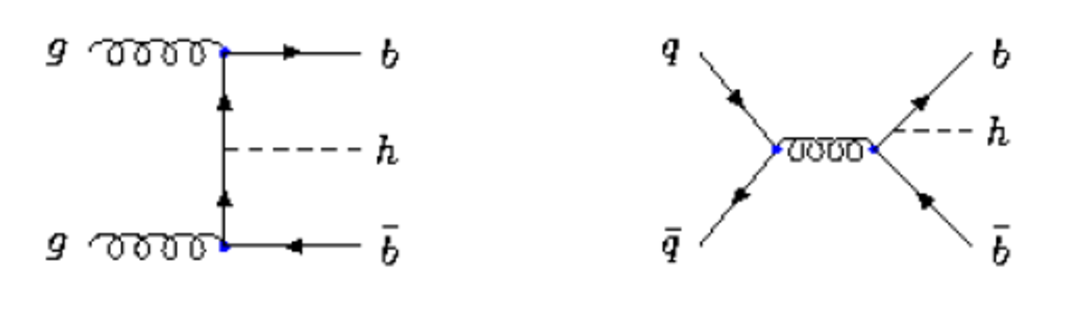
\includegraphics[width=0.5\textwidth]{Theory/FeynmanDiagrams/bbH_FeynmanDiagrams.pdf}		
	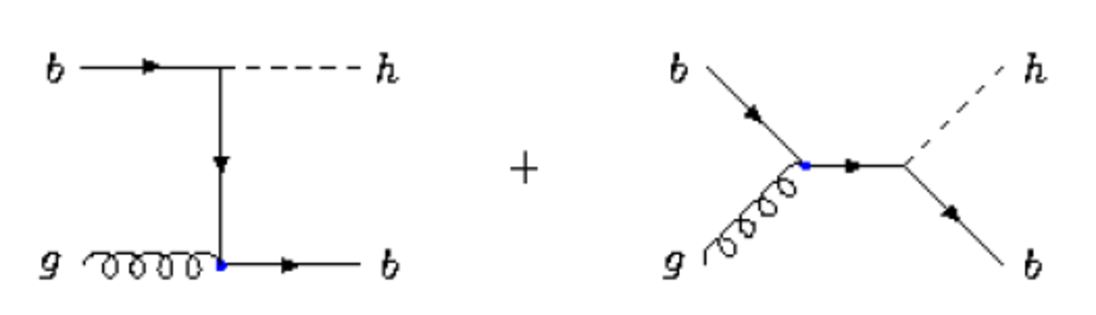
\includegraphics[width=0.5\textwidth]{Theory/FeynmanDiagrams/bH_FeynmanDiagrams.pdf}
	\caption{Feynman diagrams for leading-order production of $h$ in association with $b$-quarks.  \label{fig:fd}}
\end{figure}

Technically speaking, there is not a Feynman diagram for $H/A$ 
production that occurs in association with exactly one $b$-quark; even in 
the second set of diagrams in Figure~\ref{fig:fd} there 
is a second $b$-quark that comes from the PDF (parton distribution 
function) of the second proton.  In practice, the fourth $b$-quark 
tends to be both soft in \pt and far forward in the detector, 
making it difficult to see experimentally.  For that reason, we only require the 
presence of one $b$-quark in addition to the $b\bar{b}$ pair 
coming from the $H/A$ decay, which makes for a $b\bar{b}b$ final state.



While the behavior of the Higgs system can be complicated to fully map out, 
there are several general trends that emerge when one examines these parameters:

\begin{itemize}
	\item The cross section for $H/A$ production in association 
        with $b$-quarks increases for higher values of $\tan\beta$ (Figure~\ref{fig:xsec_vs_mass})
	\item The branching fraction of $H/A$ to $b$-quarks increases for higher values of $tan\beta$ (Figure~\ref{fig:br_vs_mass})
	\item At high $\tan\beta$, the $H/A\rightarrow b\bar{b}$ branching 
        fraction is nearly constant across a wide range of $m_A$ (Figure~\ref{fig:br_vs_mass})
	\item For a given $\tan\beta$, the production cross section falls for higher $m_A$ (Figure~\ref{fig:xsec_vs_mass})
	\item The masses of $H$ and $A$, their kinematics, 
        and the $H/A\rightarrow b\bar{b}$ 
        branching fractions are nearly the same, so that for search purposes, one 
        can treat them as one particle with $\sigma \times BR$ twice 
        that of $H$ or $A$ individually (Figures~\ref{fig:xsec_vs_mass},
        ~\ref{fig:br_vs_mass},~\ref{fig:width},~\ref{fig:TB_width})
	\item The inherent width of $H$ and $A$ increase as $m_A$ and $\tan\beta$ increase (Figures~\ref{fig:width},~\ref{fig:TB_width})
\end{itemize}





%-------------------------------------------------
\begin{figure}
	\centering
	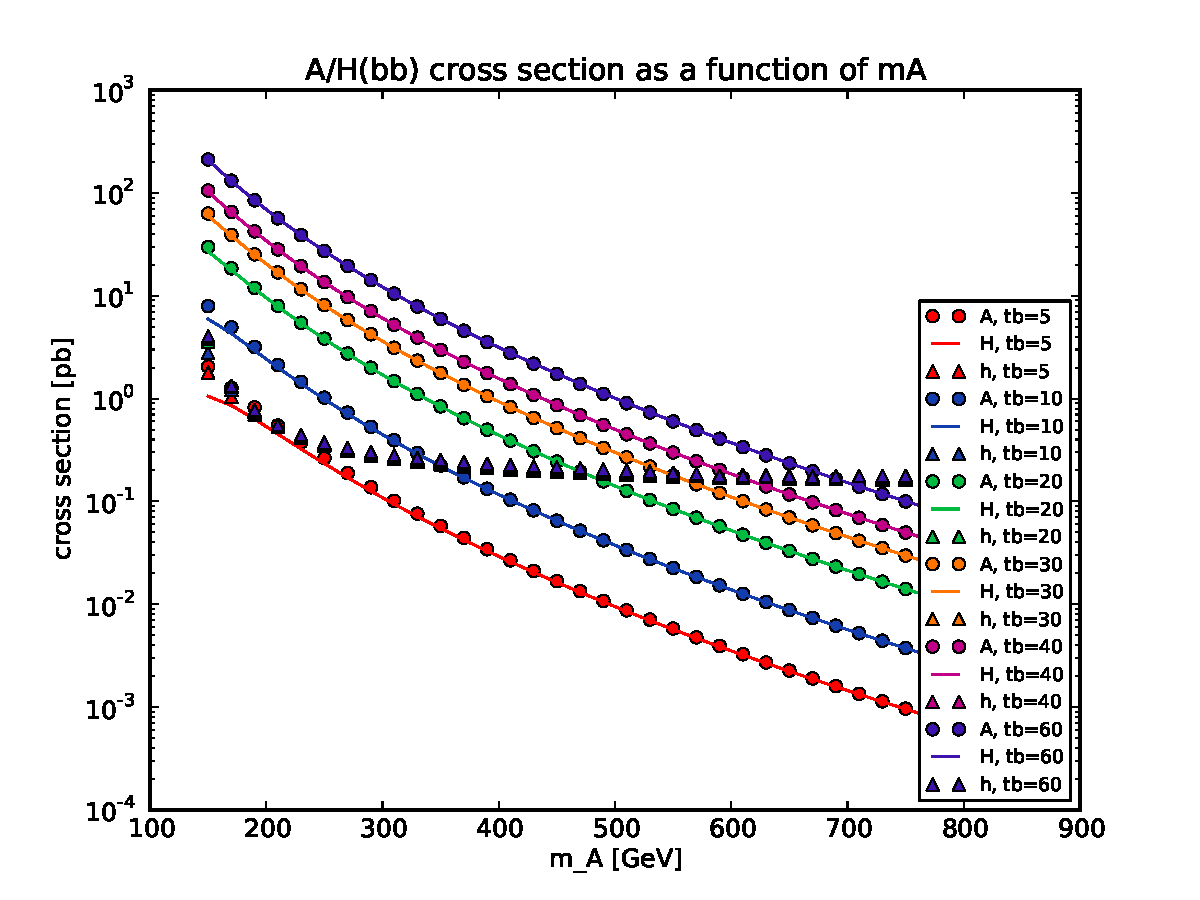
\includegraphics[width=0.8\textwidth]{Theory/figures/mssm_xsec/AH_xsec_vs_mass.pdf}
	\caption{The cross section for $b$-quark associated production of 
    $A$, $H$ and $h$ as a function of $m_A$ for several different values of $tan\beta$. 
    Figures made using FeynHiggs \cite{feynhiggs_1, feynhiggs_2, feynhiggs_3, feynhiggs_4, feynhiggs_5}.
    \label{fig:xsec_vs_mass} }
\end{figure}




\begin{figure}
	\centering
	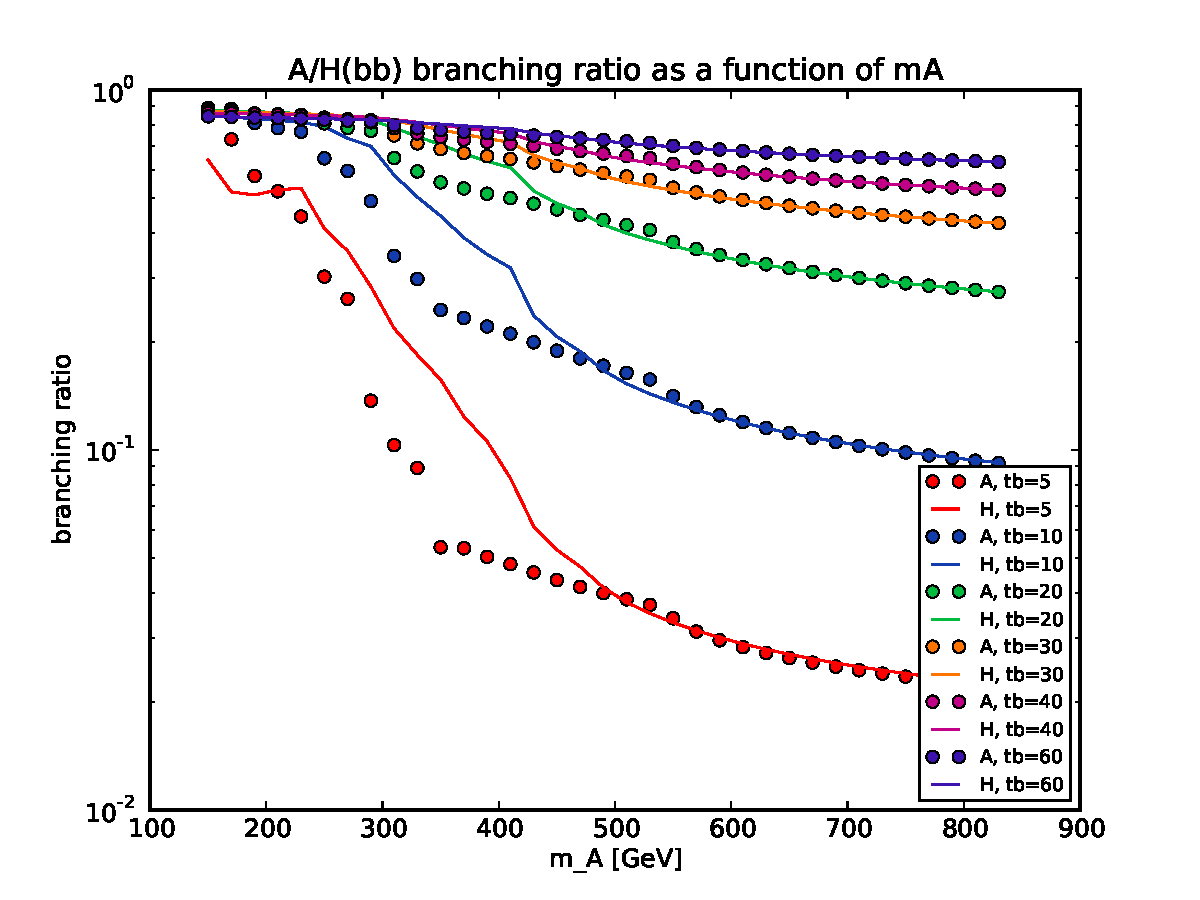
\includegraphics[width=0.7\textwidth]{Theory/figures/mssm_xsec/AH_br_vs_mass.pdf}
	\caption{The branching ratio to $b\bar{b}$ of $A$, $H$ 
    and $h$ as a function of $m_A$ for 
    several different values of $tan\beta$. The trend of higher branching 
    ratios for higher values of $tan\beta$ comes from the Higgs-to-$b$-quark 
    decay vertex carrying an enhancement factor that scales with $tan\beta$.
    Figures made using FeynHiggs \cite{feynhiggs_1, feynhiggs_2, feynhiggs_3, feynhiggs_4, feynhiggs_5}. 
    \label{fig:br_vs_mass} }
\end{figure}


\begin{figure}
	\centering
	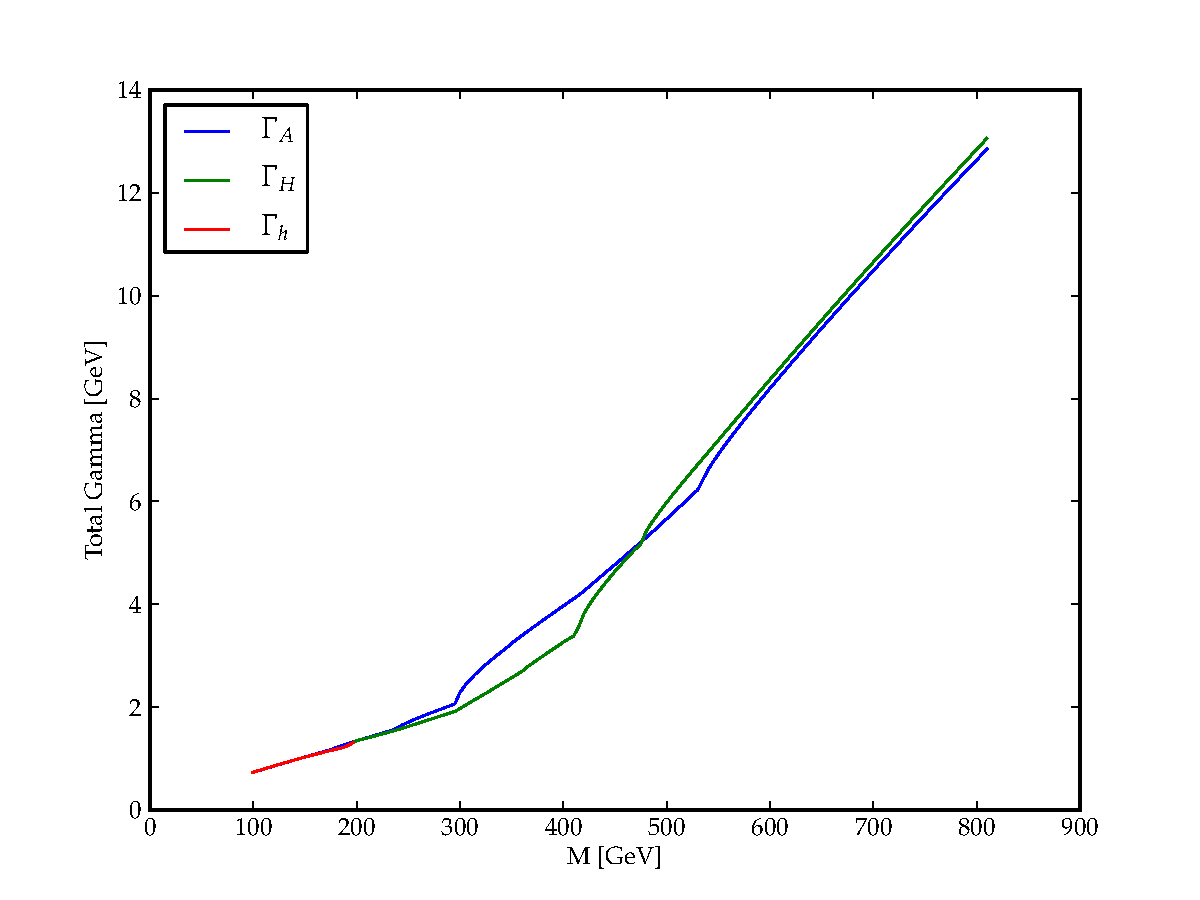
\includegraphics[width=0.7\textwidth]{Theory/figures/gamma.pdf}
	\caption{The inherent width of $A$, $H$, and $h$ 
    as a function of $m_A$ for tan$\beta$=20.  
    In practice, the inherent width of the particle is dwarfed by the experimental 
    resolution, which can be up to hundreds of GeV.  
    Figures made using FeynHiggs \cite{feynhiggs_1, feynhiggs_2, feynhiggs_3, feynhiggs_4, feynhiggs_5}. \label{fig:width}}
\end{figure}



\begin{figure}
	\centering
	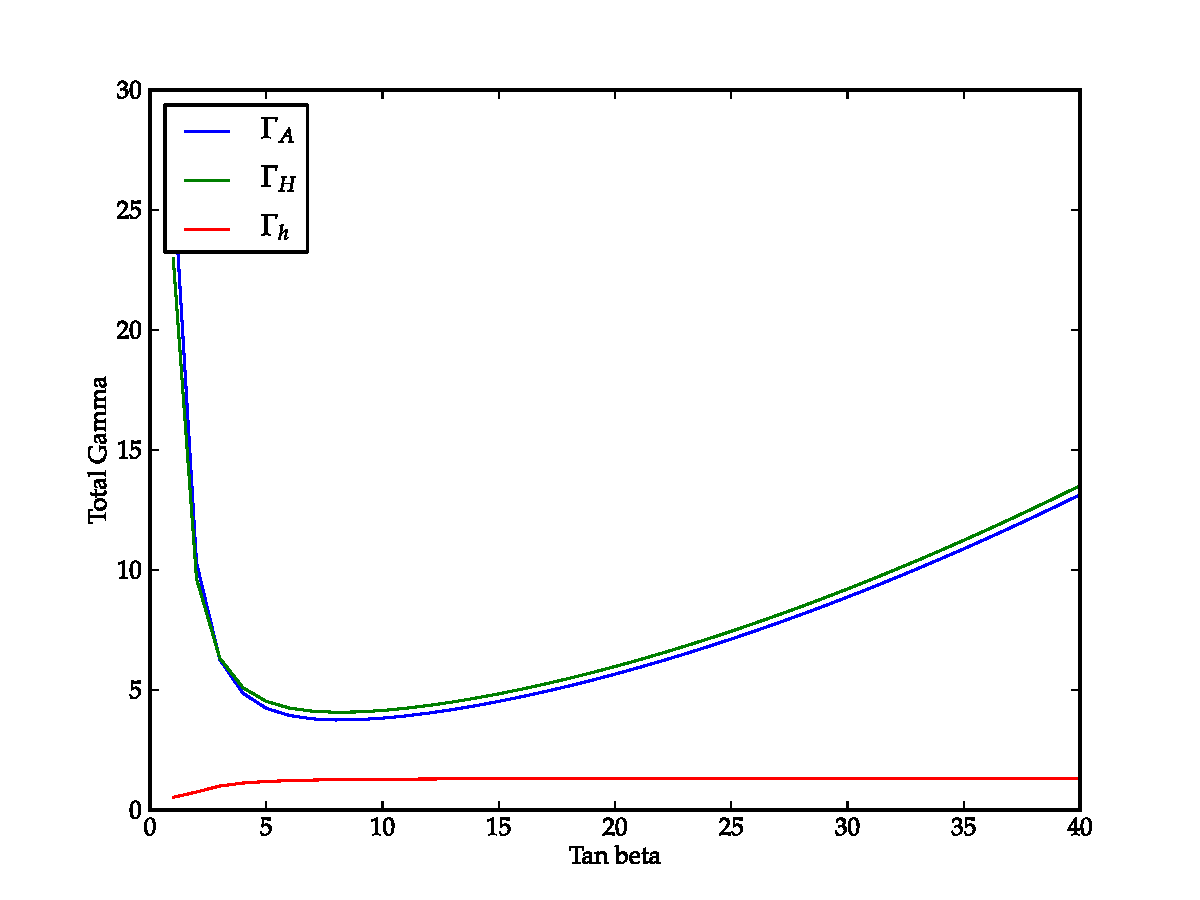
\includegraphics[width=0.7\textwidth]{Theory/figures/TB_gamma.pdf}
	\caption{The inherent width of $A$, $H$, and $h$ as a function of tan$\beta$ when $m_A$=500 GeV. 
    Figure made using FeynHiggs \cite{feynhiggs_1, feynhiggs_2, feynhiggs_3, feynhiggs_4, feynhiggs_5}. \label{fig:TB_width}}
\end{figure}
%-------------------------------------------------



%\begin{figure}
%	\centering
%	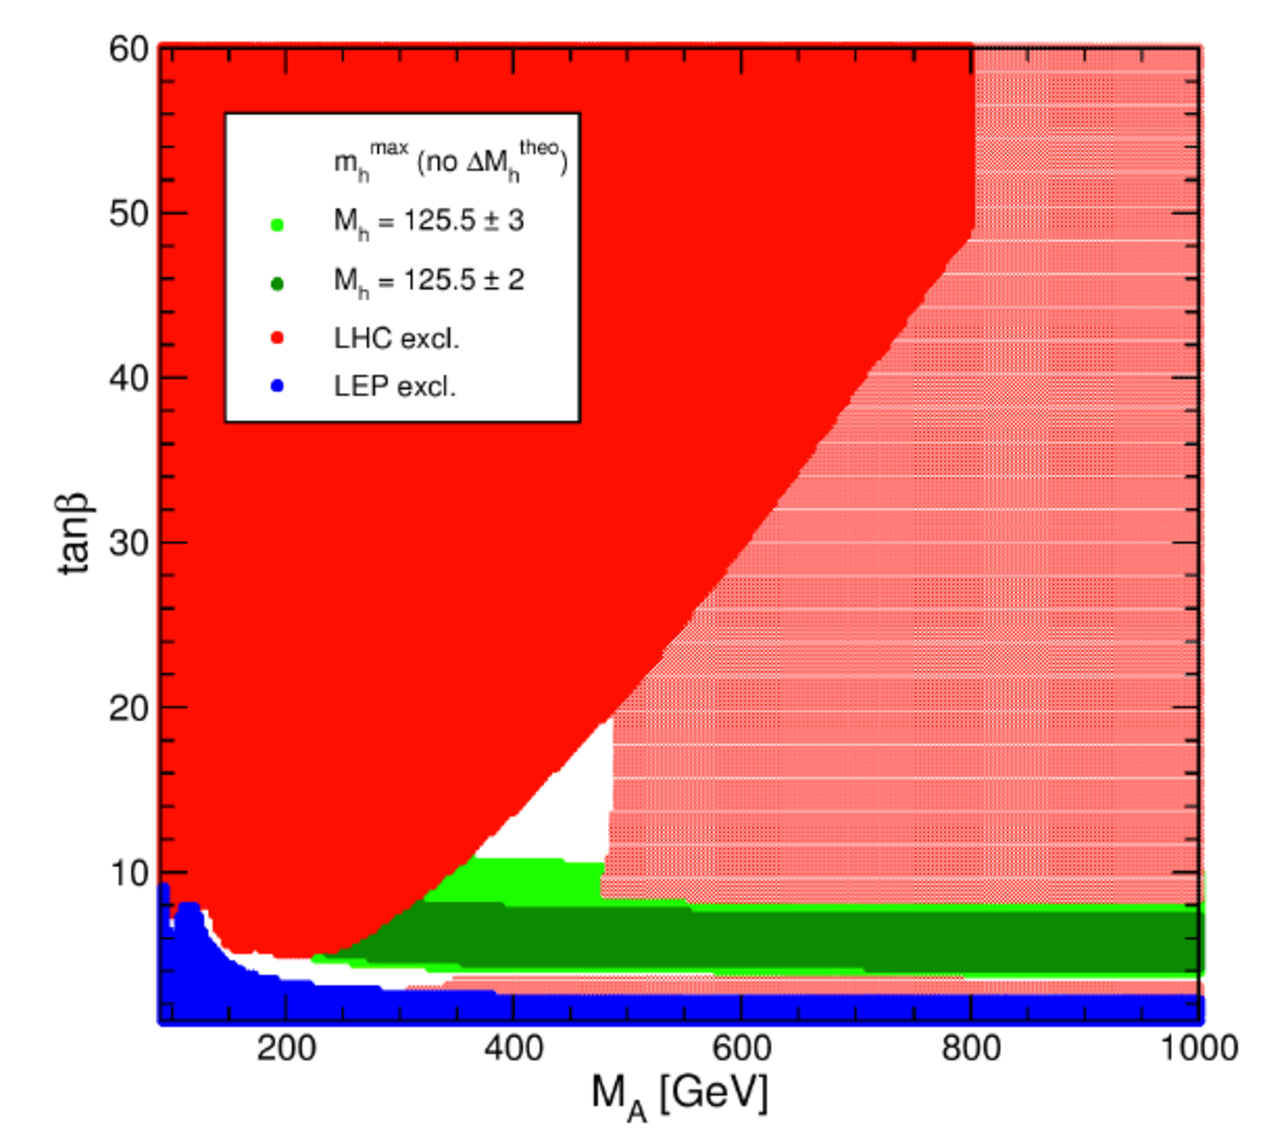
\includegraphics[width=0.7\textwidth]{Theory/figures/mh_max.pdf}
%	\caption{The favored (green) and excluded (red/blue) regions in $m_A/tan\beta$ in the $m_h^{max}$ scenario.  The red regions are excluded by LHC searches, the blue regions by LEP, and the green strip near $tan\beta$=5 is the phase space favored by $m_h$=125.5 GeV.  The fact that the green strip extends across all values of $m_A>$250 GeV means that, in the $m_h^{max}$ scenario, the cross sections of $A$ and $H$ are constrained, but the mass is only minimally restricted. \cite{Carena-2}. \label{fig:mh_max}}
%\end{figure}


\begin{figure}
	\centering
	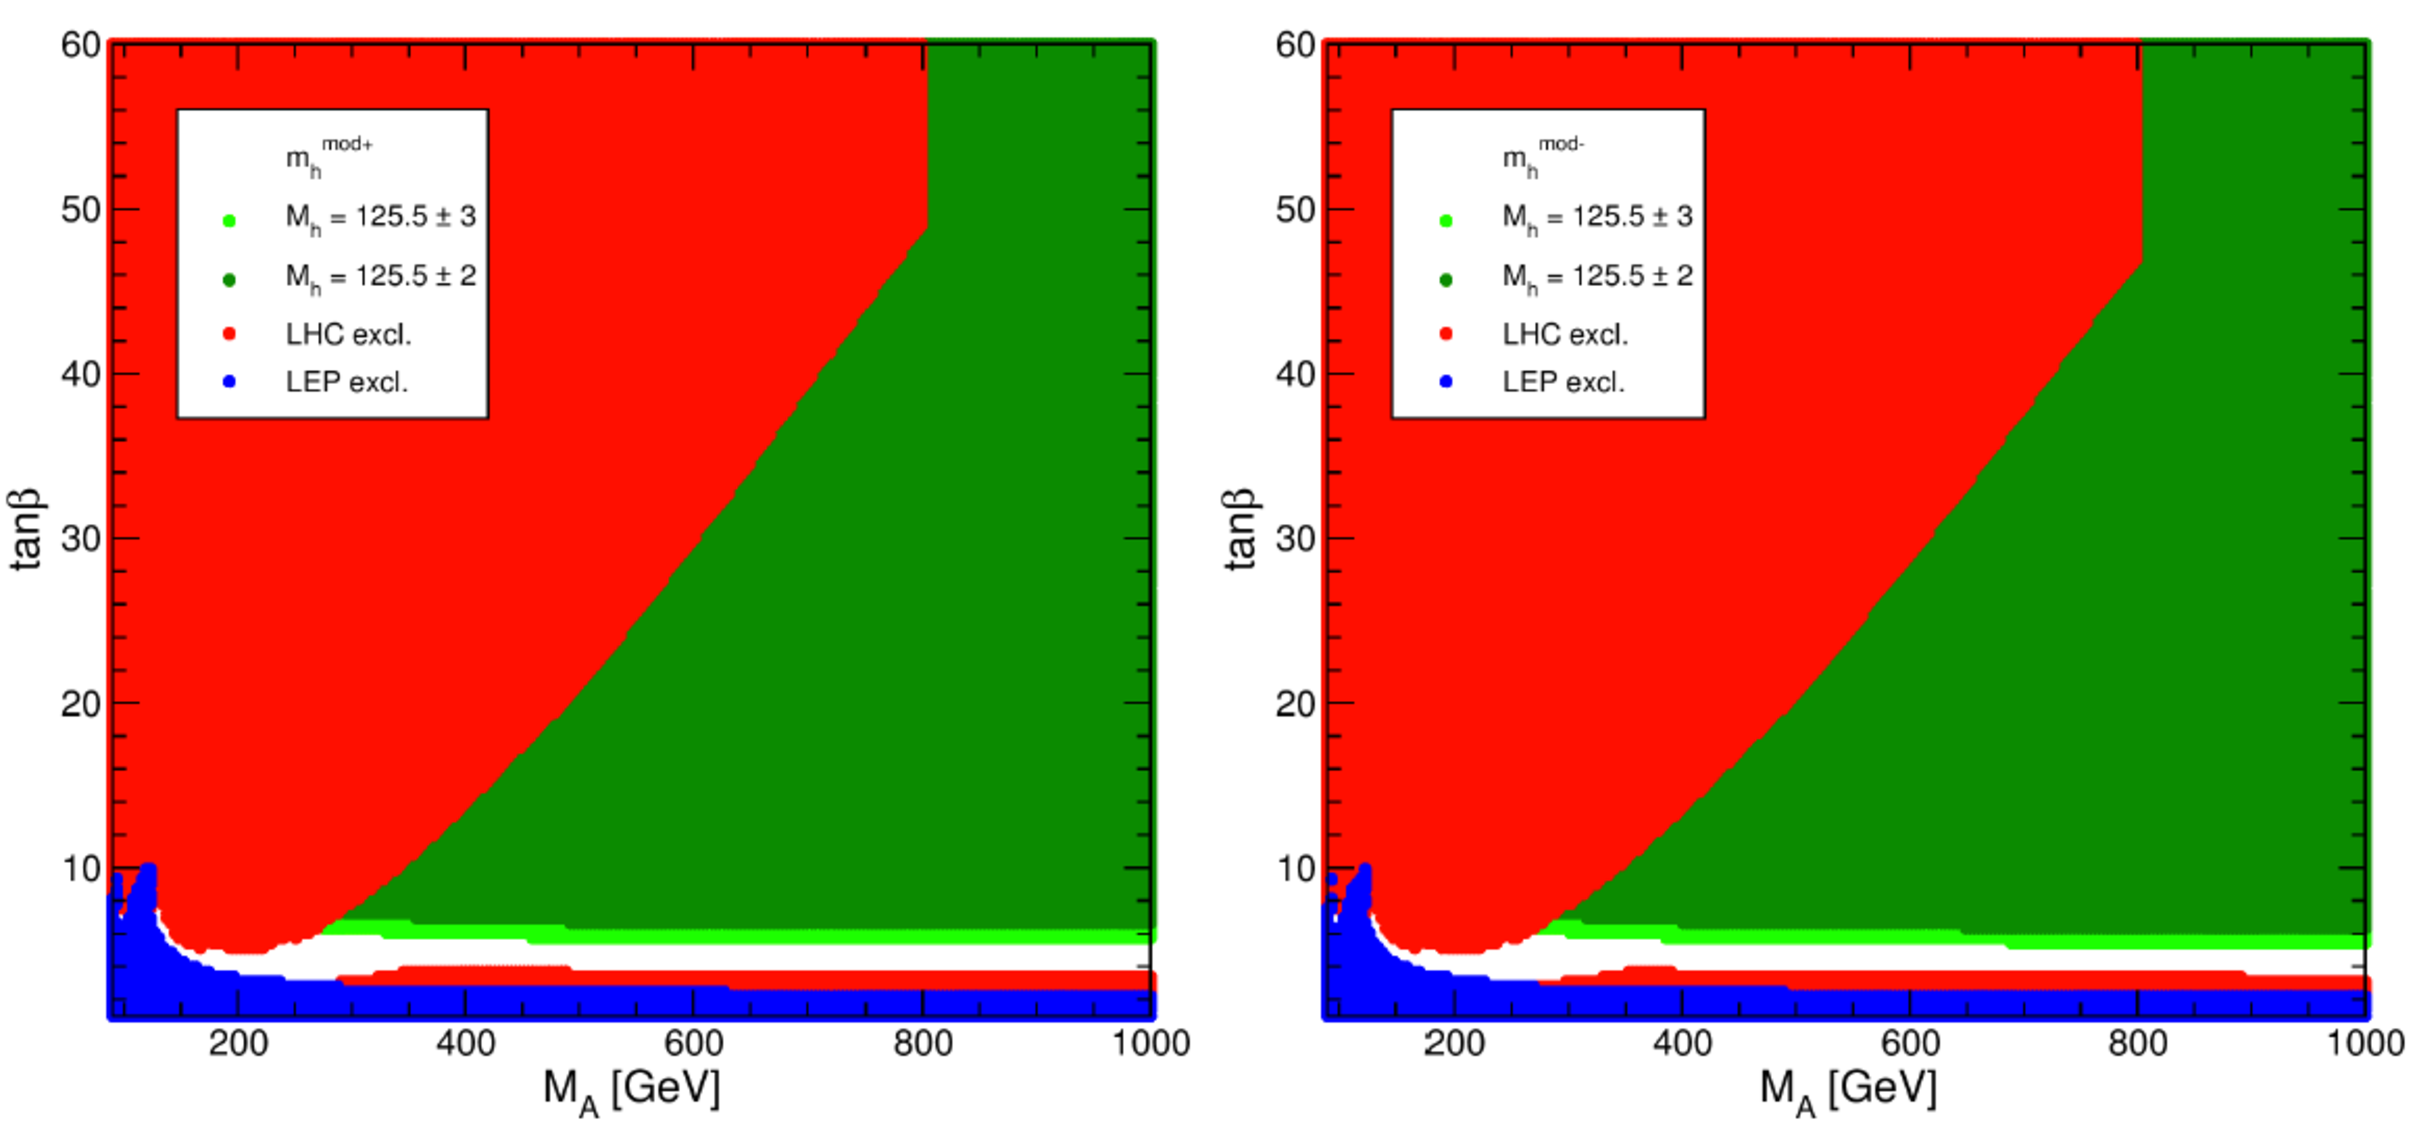
\includegraphics[width=0.7\textwidth]{Theory/figures/mh_mod.pdf}
	\caption{The favored (green) and excluded (red/blue) regions in 
    $m_A/tan\beta$ in the $m_h^{mod}$ scenario, where the green 
    region shows the phase space that is consistent with $m_h$=126 GeV.  
    After the discovery of $h$ at 126 GeV, the $m_h^{mod}$ 
    scenario is favored because it allows for $m_h$ to have 
    this relatively low value ($m_n^{max}$, on the other 
    hand, pushes $m_h$ more toward 140 GeV).  The 
    left and right plots show the topology for $m_h^{mod+}$ 
    and $m_h^{mod-}$, respectively, the details of which 
    can be found in \cite{Carena-2}. Clearly in this 
    scenario, many values of $m_A$ are open, potentially with large cross-sections. \label{fig:mh_mod}}
\end{figure}





An important and subtle point worth highlighting is that, while 
$A$, $H$, and $H^\pm$ are often called the ``SUSY Higgs bosons'', 
they are SM particles in the sense that they have R-parity of 1.  
The Feynman diagrams for the production of $H$ and $A$ 
in association with $b$-quarks can also be drawn for 
$b$-quark associated production of the SM Higgs boson $h$; 
the most important contribution of SUSY is that, when $tan\beta$ 
is large, it provides an enhancement factor to the vertices that 
drives the production cross section up to a magnitude that could be 
large enough to see in 20 $fb^{-1}$ of proton-proton collisions at $\sqrt{s}$=8 TeV.

However, that does not mean that the SUSY Higgs sector is 
independent of the details of the supersymmetric parameters.  In particular, 
it is possible that H/A decay to a pair of 
SUSY particles, such as charginos or neutralinos.  Depending on the 
scenario, the branching fraction to SUSY particles could be substantial.  
With the large number of free parameters, it is impractical to 
perform a complete scan of the MSSM parameter space, so a 
few benchmark scenarios are chosen where only $m_A$ 
and $tan\beta$ are allowed to vary, and 
the other SUSY parameters are fixed.  The leading benchmark scenario is 
the so-called $m_h^{mod}$ scenario, 
which is an update of the $m_h^{max}$ 
scenario that was used for many years.  In the $m_h^{max}$ 
scenario, the fixed SUSY parameters are assigned values that maximize $m_h$, 
the mass of the light CP-even Higgs.  However, 
in this scenario, $m_h$ is predicted to 
be around 140 GeV, while the experimentally found value is known 
to be around 126 GeV.  In order to reconcile these numbers, 
the updated $m_h^{mod}$ scenario has become 
the more useful benchmark, since it does allow for $m_h$=126 GeV.  
A comparison of the scenarios can be seen in Figures~\ref{fig:mh_max} and ~\ref{fig:mh_mod}.

Other non-MSSM scenarios also have final states with a Higgs boson
decaying to $b$-quarks and produced in association with $b$-quarks,
with cross-sections that could be seen in a few tens of inverse 
femtobarns at the LHC \cite{Gori}.   









\subsection{Constraints on $H/A$}
The discovery in July 2012 of an SM-like Higgs boson provides important constraints of the MSSM Higgs sector,
 but leaves other aspects of the theory tantalizingly unconstrained.  On the one hand, 
for many values of $m_h$, measuring the exact value of $m_h$ 
places a strong constraint on $m_A$--so once $h$ is found, one may have a good idea of what the mass of 
$A$ is, assuming the latter exists.  An important exception is when 
$m_A$ is much larger than the mass of the SM Higgs 
boson $m_h$, which is called the decoupling limit, where the 
properties of $h$ are unaffected by the existence of $H/A$.
  This means that for a light $m_h$ below 140 GeV 
or so (recall that the mass of the discovered particle is about 126 GeV),
 it is very difficult to ascertain constraints on $m_A$ by studying the properties of $h$.  
 As LHC searches advance, though, they constrain our understanding of the BSM 
 Higgs sector from a number of directions: 

\begin{itemize}
    \item Decays of $H/A$ to charginos and neutralinos only occur when kinematically 
allowed--the lack of evidence for these particles (the chargino and neutralino) below several hundred GeV suggests
that in our search region for $H/A$ (which tops out at 800 GeV) there should be little
effect from supersymmetric decays
    \item The chargino and neutralino mass limits also suggest that the higgsino mass
parameter $\mu$ is large, above several hundred GeV
    \item $B_s^0\rightarrow\mu\mu$ appears consistent with the Standard Model predictions,
placing strong constraints on the possibility of nonstandard Higgs contributions
to that decay at loop level \cite{bs_to_mumu}
\end{itemize}

Searches for the charged Higgs bosons, $H^+$ and $H^-$, also provide constraints.
In the MSSM, $H^+$ and $H^-$ are very close to $H$ and $A$ in mass, so searches
for $H^\pm$ can constrain the likely MSSM phase space available for $H$ and $A$ (Figure~\ref{fig:susy_higgs_masses}).
Outside of the MSSM, when some of the assumptions of the MSSM are be relaxed,
it is still possible to have different masses for the heavy Higgs particles.


\begin{figure}
	\centering
	\includegraphics[width=0.7\textwidth]{Theory/figures/susy_higgs_masses.pdf}
	\caption{The mass evolution of the 5 Higgs bosons of the MSSM, with the 
    mass of the Higgs-like indicated by dashed line (126 GeV).  For a large
    range of $h$ masses, the masses of $H$, $A$, and $H^\pm$ evolve very closely
    together, so searches for $H^\pm$ also can provide some indirect constraints
    on the likely masses of $H$ and $A$ \cite{ellis}. 
    \label{fig:susy_higgs_masses}}
\end{figure}
 


\section{From Beautiful Theory to Messy Experiment}

It is the experimentalist's job to understand what all this theoretical physics actually 
looks like it the detector.  This is a deep topic, and one could 
go into great detail, but a few key trends are outlined here.

First, as we've implied throughout this section, many of the particles 
for which a physicist searches cannot be seen directly--they live for a fraction 
of a second, and then decay into other particles.  Those daughter particles often 
decay themselves, and so on into a  multi-step decay chain.  Only 
the particles from the last stage in this chain actually get detected, so part 
of the physicist's job is to reconstruct the original particle(s) 
from the daughter particles.  Once the daughter particles are identified, all that is 
needed to reconstruct the parent particle is the transverse momentum (see below), energy, 
polar angle, and azimuthal angle.  These components go into a Lorentz 4-
vector for each particle, and then the Lorentz-vectors can be added together 
in a relativistically invariant way to get the mass and flight direction of the parent.

Second, certain types of particles leave distinctive signatures.  One important example is that 
particles associated with QCD, quarks and gluons, are subject to the laws of 
QCD confinement.  Once they are produced or excited in the hard scatter, quarks 
and gluons hadronize and shower.  A spray of particles, largely pions, show 
up in the detector in the general direction of the original parent quark or gluon
--if all the shower particles could be collected, they could be recombined into 
the parent particle.  These showers of particles are called jets, and are often 
named after the parent particle, such as $b$-jets, light jets 
and gluon jets.  The topic of jet reconstruction is detailed further in Section~\ref{sec:jet_reco}.  
Photons and electrons shower as well, but they generate much narrower electromagnetic showers that 
are easy to identify and reconstruct, when compared to most QCD showers.  Muons 
have the cleanest signature of all; because of their large mass, they don't 
decay before exiting the detector, so they generally make a single charged track that 
is distinctive in the dedicated muon layers of the detector.

A third important feature of particles as they appear in the detector is their $p_T$, 
or transverse momentum.  Since the initial state of each collision involves two protons, 
which are composite particles, it is impossible to know the exact longitudinal momentum of 
two quarks when they collide.  However, the transverse momentum is zero, so 
in the final state, the transverse momentum must also sum to zero.  When 
heavy particles are created and then decay, or have other particles deflecting off of 
them, the $p_T$ of the resulting particles can be tens 
to hundreds of GeV, which creates a striking signal in the detector and provides 
an experiment handle when trying to understand the event.

The main challenges of this particular search arise from several features of the search.  
First, the final state is all-hadronic, where reconstruction is difficult and 
the QCD background is large.  Second, since the mass of $H$ 
and $A$ are relatively unconstrained, a search has to span a large 
range in $m_A$ in order to be sensitive to discovery.  
Third, the combinatorics of selecting the correct two $b$-jets for reconstruction 
(from the three or more available in an event) require dedicated study.  


\section{Previous Searches}
Searches for $A$ and $H$ in this final state have been performed at the Tevatron
as well as CMS.  The searches at the 
Tevatron were particularly tantalizing because both CDF \cite{CDFbH} and D0 \cite{D0bH} spotted 
slight excesses of events, around 2$\sigma$ standard deviations each, between approximately
100 and 150 GeV.  The LHC experiments (ATLAS and CMS) present an opportunity to
re-examine the same region of phase space, albeit with higher integrated luminosity
and center-of-mass energy.  CMS does not observe an excess in the 100-150 GeV range 
when searching over approximately 5 $fb^{-1}$ of data at $\sqrt{s}$=7 TeV \cite{CMSbH}.

This analysis serves as an important update and extension of the searches done
in other experiments.  Due to differences in the triggers for these analyses,
the ATLAS search does not have access to $m_A$ values below 400 GeV, but it does 
provide the first limits between 400-800 GeV.  This analysis is also the only
search at $\sqrt{s}$=8 TeV, and searches over an integrated luminosity (19.5 $fb^{-1}$)
that is about 4 times higher than the next largest search, done at CMS.


 








% Activate the following line by filling in the right side. If for example the name of the root file is Main.tex, write
% "...root = Main.tex" if the chapter file is in the same directory, and "...root = ../Main.tex" if the chapter is in a subdirectory.
 
%!TEX root =  ../Thesis.tex

\chapter[ATLAS Detector]{CERN, the LHC Accelerator and the ATLAS Detector}




\section{Introduction}
Experimental particle physics research has many prominent features, but the most prominent
might be the scope and collaborative nature of the work.  This thesis is one of many that have
been produced at the ATLAS dectector at CERN, and makes use of the dedicated work of many
physicists to build and maintain the experimental apparatus and data processing pipeline.
The Large Hadron Collider is the first major piece of this, where beams of protons are accelerated to
tremendous energies and the smashed into each other inside the cavernous detectors, including ATLAS.
It is the collisions
between individual pairs of protons that underpin the entire scientific mission: in this environment,
interesting and rare physics can result from the interactions between the protons.  It is the mission of the
LHC to generate large numbers of high-energy proton-proton collisions, and then the mission of the detectors
to record and analyze the data that results from the collisions.  



%http://home.web.cern.ch/about/accelerators
\section{CERN and the Large Hadron Collider}
\label{sec:cern_lhc}
The European Center for Nuclear Research (CERN) is a scientific complex in Geneva, Switzerland that was established 
in the years following World War II.  Its focus is experimental particle physics, in particular the Large Hadron 
Collider (LHC), and it has a long and storied history of producing particle discoveries and other scientific
advances.

The LHC is the particle accelerator that serves as the centerpiece of CERN's scientific program.  The accelerator is 
an RF-driven circular sychrotron located in an underground tunnel with a circumference of 27 km, and when 
it is running, accelerates and collides two proton beams (sometimes two lead ion beams, but we will 
focus on the protons in this thesis) at four interaction points around the accelerator ring.  Each of proton beam 
contains thousands of bunches of protons which are very deliberately spaced so that every 50 ns, two 
of those bunches going opposite directions will overlap at one of the interaction points.  In 2012, the energy
of the proton beams was 4 TeV each, making for a total of 8 TeV of energy when the beams are collided head-on.
These are the highest-energy proton-proton collisions ever created by man-made acceleration, and reliably making lots of
collisions is a scientific and engineering endeavor completely in its own right, even before considering
the physics insights that we get as a result.


There are two major figures of merit for any particle accelerator: energy and luminosity.  Energy is typically limited 
by the circumference of the accelerator and by the magnetic field strength of the accelerator's bending magnets.  
The record-breaking energy of the LHC is a function of its tremendous size (27 km in circumference) as 
well as 1232 8.4 tesla superconducting dipole magnets that keep the beams in place within the accelerator.  Luminosity 
 is a measure of how many collisions the accelerator can produce, with higher luminosities meaning that more 
interesting events (and non-interesting events!) can be generated.  Since different processes happen at different rates
, the rate at which a given process occurs is usually stated in terms of its production cross section.  
Cross sections are measured in units of barns (or fractions thereof), with one barn being equal to 10
$^{-28}$ $m^2$.  Luminosity is measured in inverse barns, so that he cross section 
can be multiplied by the luminosity to give a total number of events for that type of event.  Luminosity 
is usually limited by the intensity and focus of the beam, and the bunch crossing rate.


%http://inspirehep.net/record/805147/plots
\begin{figure}
	\centering
	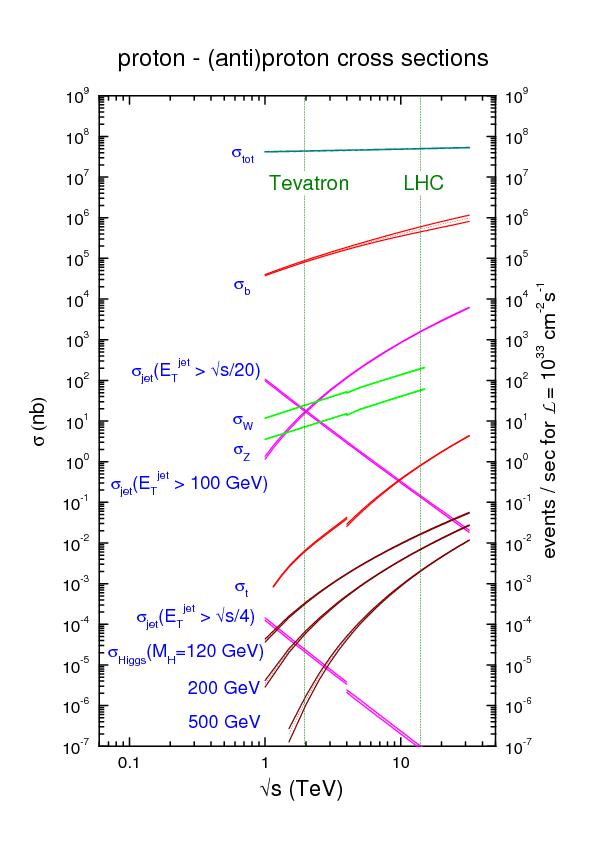
\includegraphics[width=0.6\textwidth]{ATLASDetector/images/crosssections2008.png}
	\caption{Cross sections for various processes as a function of center-of-mass energy
            of the original collision.  The ``skip'' at 4 TeV occurs because below that
            value, the cross sections are for proton-antiproton collisions like those
            made at the Tevatron, while higher energy collisions are being produced
            at the LHC. \label{fig:cross_sections}}
\end{figure}


Energy and luminosity go hand-in-hand to push back the frontiers of physics.  One of the 
major goals of the LHC is to discover new particles, and by conservation of energy the higher the LHC 
can go in energy, the heavier it can go in new particles to potentially create.  Another important fact 
is that, while cross sections for all types of processes typically go up as the collision energy increases, 
many new physics models have production cross sections that go up faster than the backgrounds as a function of center
-of-mass energy.  In other words, for a given process, the signal-to-
background ratio tends to go up as energy increases so new physics can be much easier to spot at higher 
energies than at lower energies.   

Discovery reach can also be extended by increasing the luminosity of a machine, 
since sensitivity to a signal is typically defined as $s/\sqrt{b}$--for example, a 
10-fold increase in luminosity means a $\sqrt{10}$-fold increase in a search's sensitivity.  
Luminosity can be increased by either tuning the accelerator to have a higher instantaneous luminosity, with a more focused 
beam or higher beam current for example, or by simply running the machine for a longer time.  In 
practice, increasing instantaneous luminosity at the LHC also means increasing the number of lower
-energy collisions that, while not of physical interest, still get picked up in the detector (pileup
).  The removal of pileup is an intense and dedicated effort that will be addressed in Section~\ref{sec:pileup}.



%%% lumi in 2010, 2011 and 2012
\begin{figure}
	\centering
	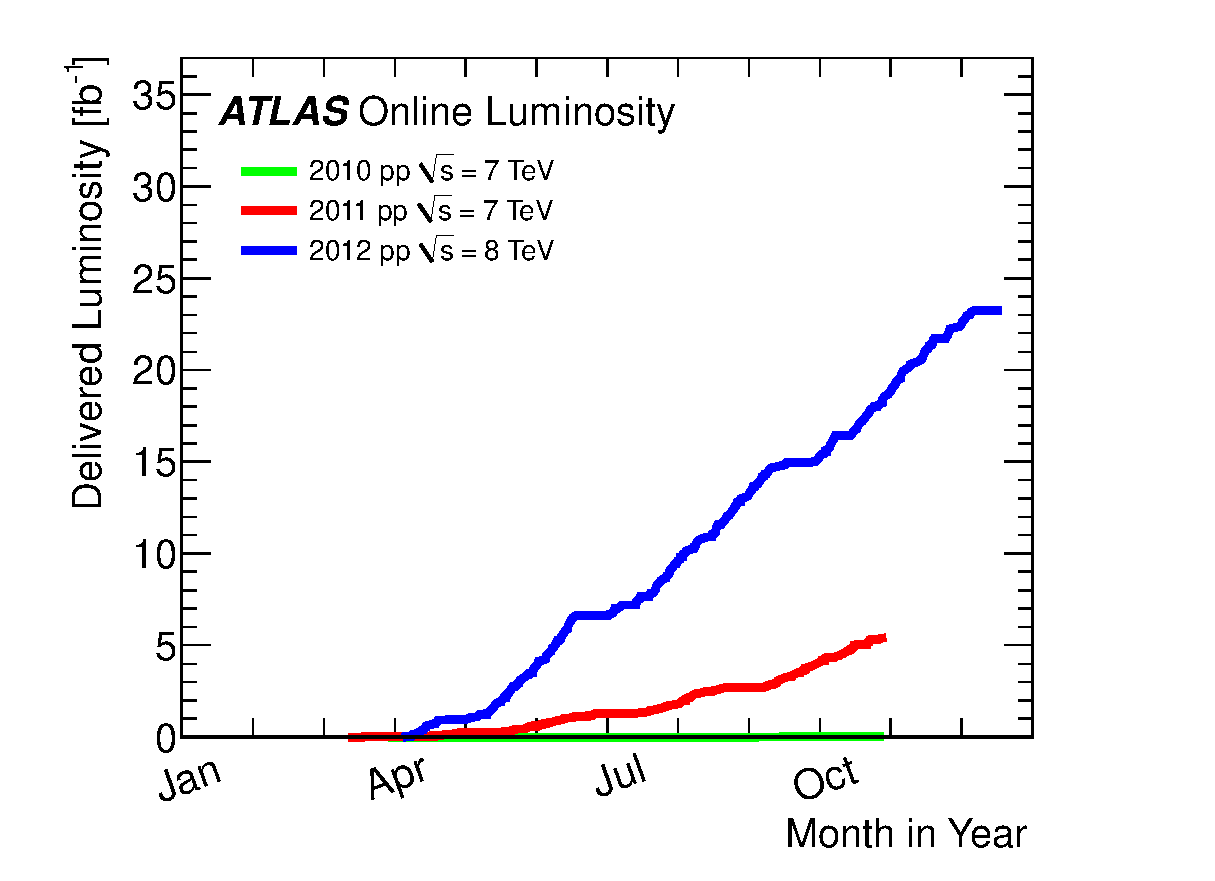
\includegraphics[width=0.6\textwidth]{ATLASDetector/images/intlumivsyear.eps}
	\caption{The luminosity collected in 2010, 2011 and 2012 at ATLAS. \label{fig:lumi_vs_year}}
\end{figure}



The LHC is only the last in a chain of accelerators, which all work together to create the high 
energy and luminosity that we associate with the LHC.  The first step in the process is the proton source
, where hydrogen atoms are subjected to an electric field that separates the protons from the electrons.  Then the 
protons are accelerated by a 90kV field and focused, and fed into a linear accelerator.  From this point 
forward, all the accelerators use radio frequency (RF) electromagnetic waves to impart energy to the protons.  

The linear accelerator brings the protons up to an energy of 50 MeV, then they go to the Proton 
Synchrotron Booster (up to 1.4 GeV), and then the Proton Synchrotron (25 GeV).  Then 
the protons are passed to the Super Proton Synchrotron, where they reach an energy of 450 GeV, and 
finally the beam is split into half and each half is injected into the LHC going a different direction.  
Figure ~\ref{fig:accelerator_complex} shows all the major accelerators at the CERN site.



%%% CERN accelerator figure
\begin{figure}
	\centering
	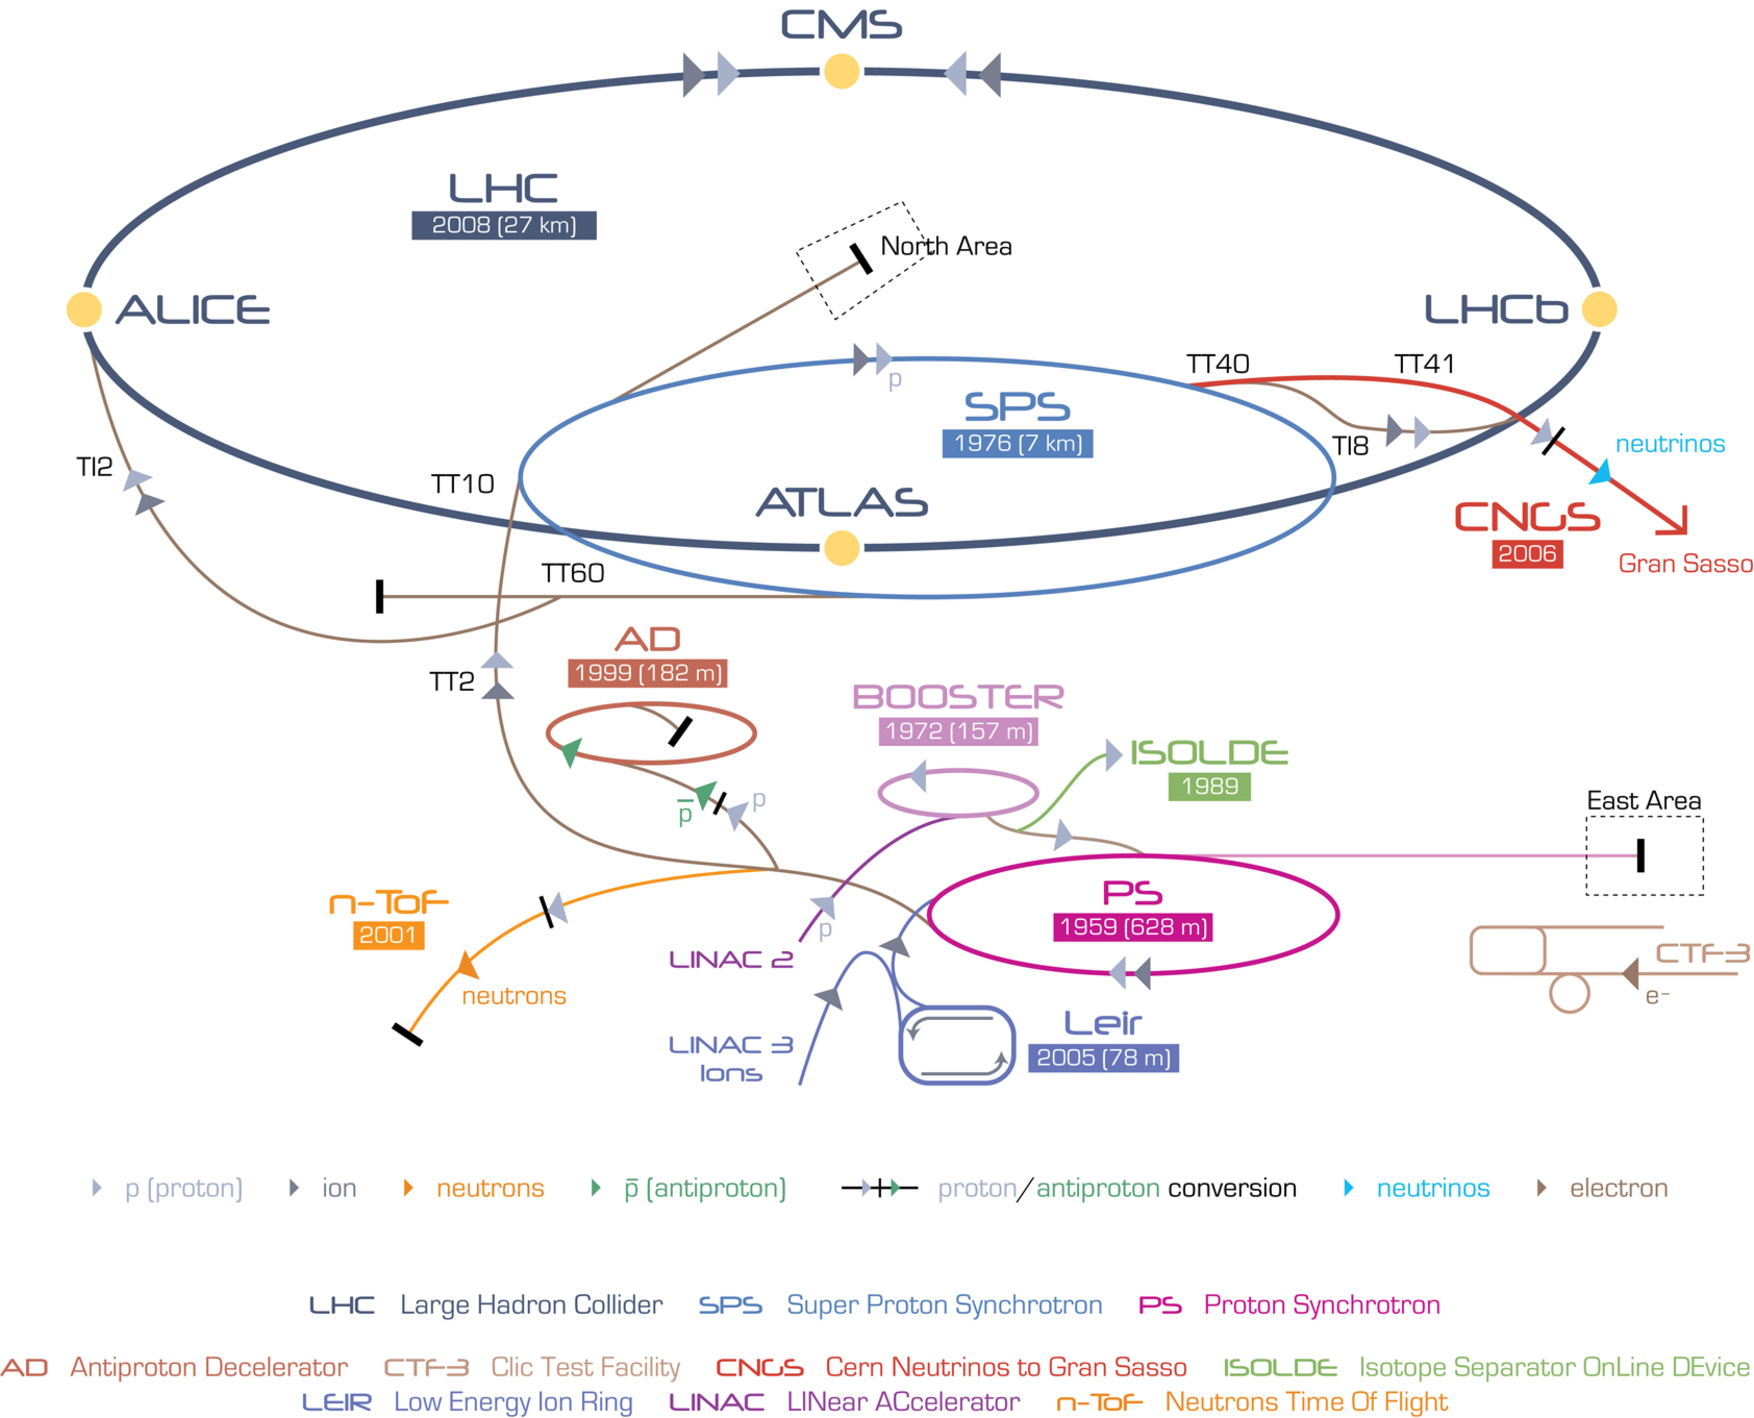
\includegraphics[width=0.8\textwidth]{ATLASDetector/images/Cern-Accelerator-Complex.pdf}
	\caption{ The major elements in CERN's accelerator complex, which turns ordinary hydrogen atoms in the highest-energy man-made collisions ever made. The four interaction points, labeled for their respective experiments (ALICE, ATLAS, LHCb and CMS) can be seen around the perimeter of the LHC. \label{fig:accelerator_complex}}
\end{figure}



Once the beams are in the LHC, they are accelerated up to the full collision energy of 4 TeV 
per beam.  Then the beams are focused  and carefully steered into position so that head-on collisions commence
.  The protons are arranged in bunches within the beams, with each bunch 50 ns away from its neighbors
, so that the collision frequency within the detectors is 20 MHz.  The data-taking is organized into 
runs, where collisions are created continuously for up to 16 or so hours at a time.  A run 
typically ends either when enough of the beam gets burned away by the collisions that the instantaneous luminosity drops and 
it becomes worthwhile to refill, or when a technical glitch causes the beams to be dumped.

The history of the LHC is a dramatic one.  The LHC first turned on in 2008, but within 
days had to shut down following a catastrophic failure of the bus bar between superconducting magnets.  It restarted in 
2009 at 7 TeV, half the design energy of 14 TeV (a repercussion of the accident), and 
the first run for physics was performed in 2010, with a total dataset size of 36 inverse picobarns.  
The progress in 2011 was dramatic, as the beam intensity was steadily increased over the course of the run 
to create an exponential increase of the luminosity recorded, and at the end of 2011 the total dataset size 
was about 5 inverse femtobarns (a factor of more than 1000 greater than the data recorded in 2010).  
The progress continued in 2012, with a slightly increased energy of 8 TeV and about 20 $fb^{-1}$ 
collected, culminating in the 4 July 2012 announcement of the discovery of a new particle, later confirmed to 
be the long-sought Higgs boson.  The total collected luminosity is illustrated in Figure~\ref{fig:lumi_vs_year}.  
At the end of 2012, the LHC commenced a 2-year shutdown to complete upgrades and repairs, 
with the intention of starting up again in 2015 at 13 TeV and 25 ns spacing between bunch crossings.
When the LHC starts up again, the search for new particles will begin again as both energy and luminosity
records are broken by the upgraded machine.



\section{The ATLAS Coordinate System}
The ATLAS detector is situated at Point 1 of the LHC ring.  Since the detector has a cylindrical shape
, polar coordinates are the most natural basis for describing its geometry.  The radial direction (usually notated ``r'') 
is defined as the vector originating at the interaction point, in the middle of the detector, and pointing 
transverse to the beamline.  The azimuthal angle $\phi$ and the polar angle $\theta$ complete the 
coordinate system, although in practice it is more common to use pseudorapidity $\eta$ instead of $\theta$.  
Pseudorapidity has the advantage of being a quantity that is Lorentz-invariant under boosts longitudinal to the incoming beams 
(in a hadron collider, the longitudinal component of the momentum of the incoming partons is not known).  
The definition of pseudorapidity $\eta$ is

\begin{equation}
\eta = -ln(tan( \frac{\theta}{2} ))
\end{equation}

Since the proton is a composite particle, made of three valence quarks and an indeterminate number of gluons, even 
if the proton has a known energy, its constituent partons can have a wide range of energies.  In 
general, then, the exact collision energy can vary from event to event, and outgoing particles can be 
boosted forward in $\eta$.  However, energy is conserved in the $\phi$ dimension, so transverse 
energy and momentum ($E_T$ and $p_T$, respectively) should add up to zero in events where there are no particles escaping detection.

\section{The ATLAS Detector}
The ATLAS detector is like an onion: it has layers, and it makes you cry.  There are 
several main subsystems, each of which is designed to measure a certain characteristic (charge, momentum, energy
, etc.) of a particular type of particle (quark, electron, muon, etc.).  The subsystems 
work hand-in-hand with the trigger and data acquisition system, which handles the decision-making 
of which events to record and goes about writing those events to disk.  

\subsection{Inner Detector}
The innermost layer of the ATLAS detector is the tracker, which provides precision measurements of the trajectories of charged 
particles.  As a charged particle traverses the layers of the tracker, it ionizes the detector material which creates 
small electrical signals that can be amplified and read out by the system.  These so-called ``hits'' 
are combined during reconstruction into tracks, which represent the paths of particles like electrons, muons, and charged 
pions in the detector.

The information from the tracker is used in particular to determine the transverse momentum (p$_T$) of 
charged particles, and to perform particle identification.  The tracker consists of three primary subsystems: the pixels, 
semiconductor tracker (SCT), and transition radiation tracker (TRT).  A charged particle created at or near the 
interaction point would typically travel through all three subsystems, creating some number of hits in each one.  On 
average, a track has 3 pixel hits, 8 hits in the SCT (4 double-sided hits
) and about 34 hits in the TRT, with all the inner detector subsystems enclosed by a 2 tesla solenoidal magnetic field. 


\begin{figure}
	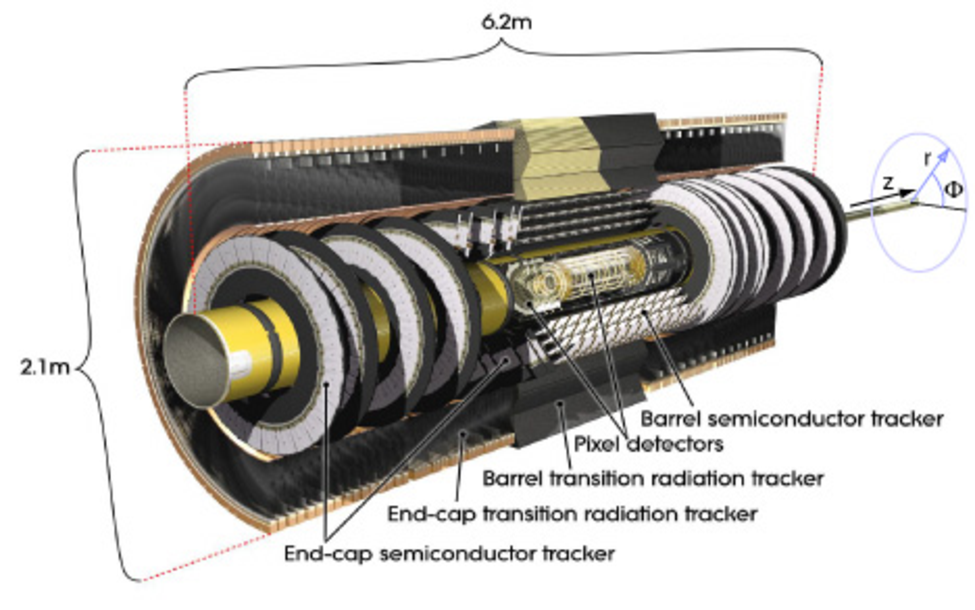
\includegraphics[width=0.8\textwidth]{ATLASDetector/images/innerDetector.pdf}
	\label{fig:inner_detector}  
	\caption{A cutaway picture showing the main components of the ATLAS inner detector.  The ATLAS coordinate system is sketched on the right-hand side of the figure.}
\end{figure}


%http://cds.cern.ch/record/1290332/files/VERTEX%202010_015.pdf
\subsubsection{Pixel System}
\label{sec:pixel}
The pixel system sits physically closest to the beam line and interaction point.  It is built of silicon pixels 
that measure 50 x 400 micrometers each, which are organized into sensors.  Each sensor contains 46,080 
pixels, and then there are 16 sensors organized onto a pixel module.  The pixels as a whole contain 1744 
modules, organized into 3 layers each in the barrel and the two endcaps.  
The pixel system in aggregate contains 80 million channels and measures about 1.4 meters long by 0.4 meters in diameter.

\begin{figure}
	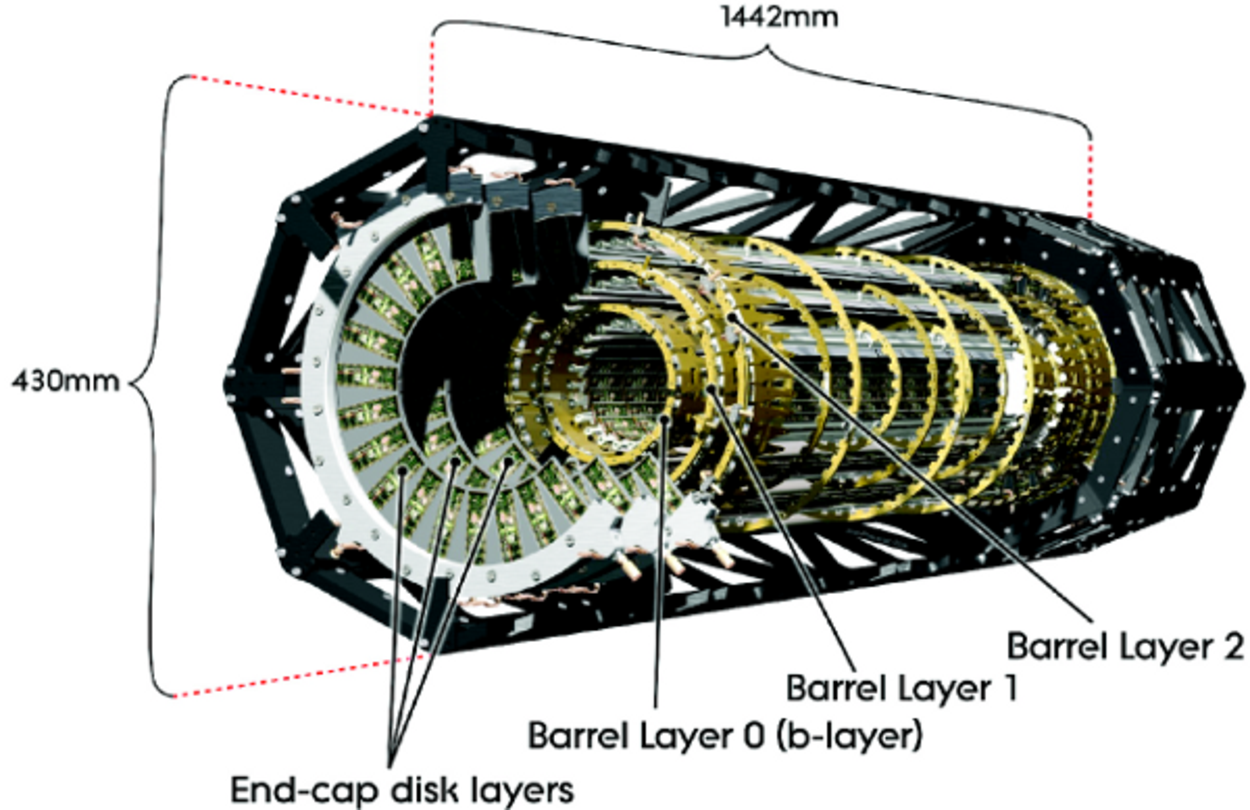
\includegraphics[width=0.8\textwidth]{ATLASDetector/images/pixel_detector.pdf} 
	\caption{A picture showing the main layers of the ATLAS pixel detector, including the disk layers on the end.  Starting in 2015, a 4th layer, the insertable b layer (IBL), will be inserted inside the current layer 0. 	\label{fig:inner_detector} }
\end{figure}

% http://iopscience.iop.org/1748-0221/3/07/P07007/pdf/1748-0221_3_07_P07007.pdf
The pixel technology is designed to give high-precision measurements of the location and momentum of charged tracks.  
A pixel module has two main components, the silicon sensor and the front-end chip, which are 
bump-bonded together.  When a charged particle traverses the sensor it ionizes silicon atoms, creating 
electron-hole pairs, and then a bias voltage applied across the sensor causes the electrons and holes 
to drift to opposite sides of the sensor, where they can be read out by the front-end chips.  

The pixel readout is based on detecting and quantifying this ionization current.  A particle with greater momentum will create 
more electron-hole pairs and thus a longer readout pulse, which passes through a preamplifier and then a 
discriminator.  The discriminator is set with a tunable threshold number of electrons, typically a few thousand, and 
the signal metric is then the length of time for which the pulse was above that value (called ``
time over threshold'', or TOT).  Having a threshold in place helps distinguish ionization current from leakage current, 
which occurs when the silicon does not have robust insulator characteristics and current begins to flow across the sensor even 
when there is no ionizing particle present.  One important effect of radiation damage to the pixel detector is that 
it damages the silicon, allowing for increases in leakage current up to 100 nA, so over the course 
of large radiation doses to the detector the thresholds sometimes have to be raised to compensate for the damaged material.  


%from atlas TDR
\begin{wrapfigure}{R}{0.5\textwidth}
  \begin{center}
%\begin{figure}
	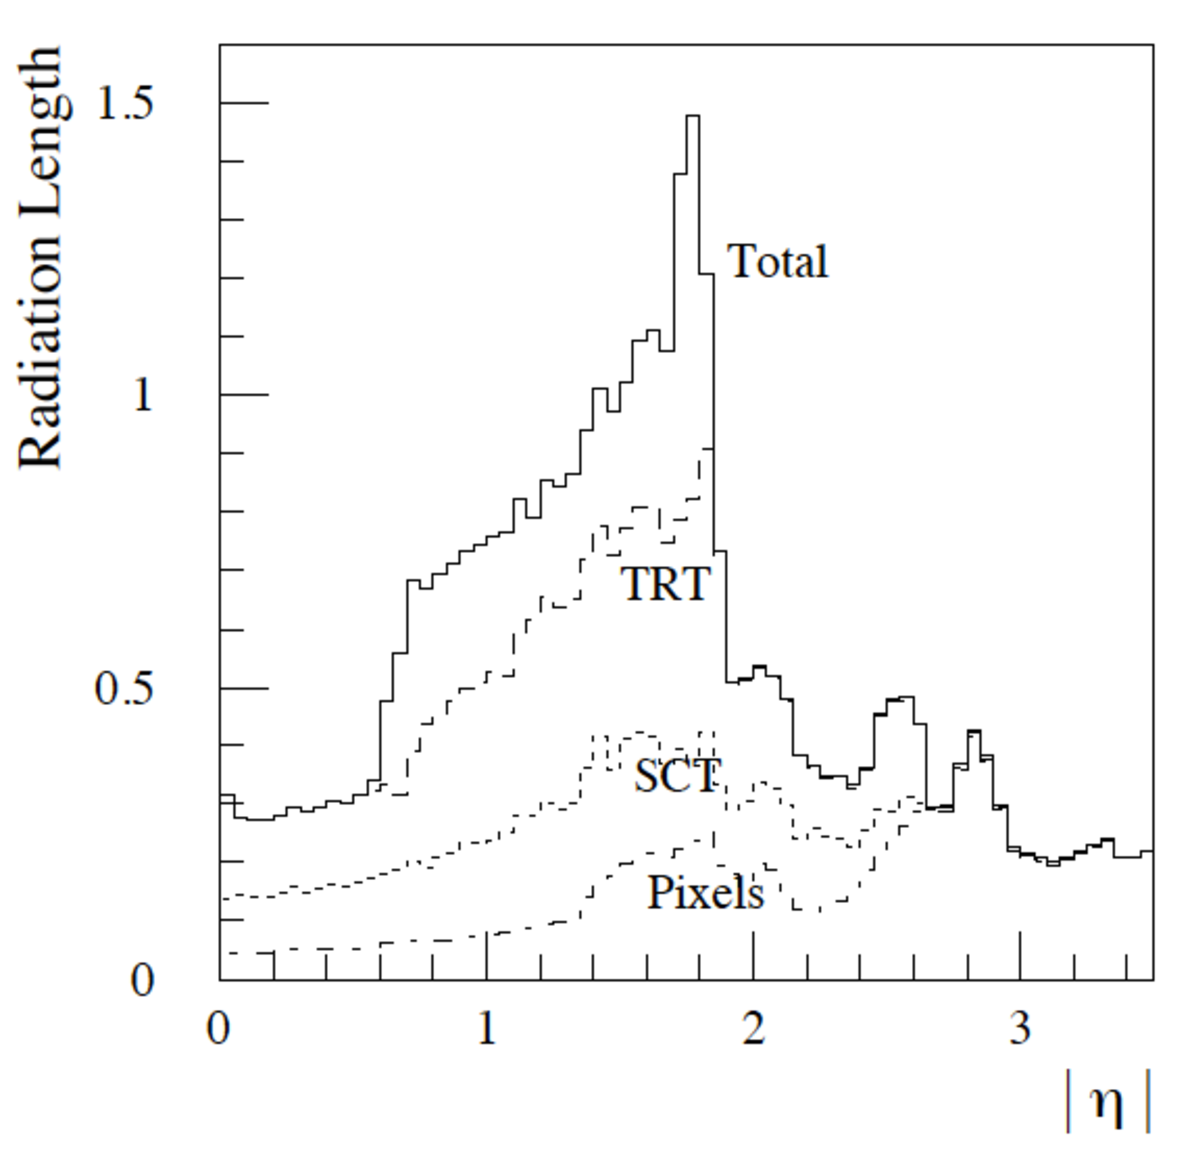
\includegraphics[width=0.45\textwidth]{ATLASDetector/images/id_material_budget.pdf}
	\label{fig:id_material}
	\end{center}
%\end{figure}
\end{wrapfigure}

Another important consideration when designing and constructing the pixel detector is the material budget of the system.  When a 
charged particle traverses the pixels, interacting with the silicon, its trajectory can change by virtue of these interactions 
as it undergoes multiple scattering or secondary interactions.  This can be a problem, for example, when reconstructing 
tracks--if a track has a kink from where it scattered off detector material, it will be more 
challenging to reconstruct the track or correctly measure its momentum.  These material effects are particularly important for the pixel 
detector, because they are the first layer of detector traversed by particles after they leave the collision point.  
One way to mitigate these effects is to place high-material components, such as power supplies and readout 
electronics, in more forward regions so that they are not in the path of central tracks.  There are 
two figures of merit when evaluating the material budget of a system: the radiation length is the distance an 
electromagnetically interacting particle (such as an electron, positron or photon) travels before losing 1/$e$ 
of its energy to bremsstrahlung, while the interaction length is the mean distance traveled by a hadronically-interacting 
particle (such as a proton, neutron or pion) before undergoing an inelastic nuclear interaction.  Figure ~\ref{fig:id_material} 
of the material volume, in units of radiation length vs. $\eta$, shows that the material budget 
(especially pixels) is minimized in the most central regions.


%https://cds.cern.ch/record/1445527/files/ATL-COM-PHYS-2012-471.pdf
The pixel system all together provides fine resolution of the beamspot and surrounding area, which serves several important purposes
.  First, since there are typically many hard p-p collisions in each bunch crossing, the pixels 
system has longitudinal resolution $z_0\sin\theta\approx$0.05-0.3 mm 
enables the reconstruction of multiple primary vertices that are typically separated by a few millimeters \cite{pixel_res}.  This 
is critical for controlling pileup in the high-luminosity LHC environment.  Second, the transverse resolution of 0.01-0.1 mm 
enables the track resolution required to allow precision b-tagging for identification of bottom quarks.  More details
on both the track reconstruction and the $b$-tagging methodology can be found in Sections~\ref{sec:trk_reco} and ~\ref{sec:b-tag}. 


% useful thesis: http://www-pnp.physics.ox.ac.uk/~demirkoz/thesis.pdf
\subsubsection{Semiconductor Tracker (SCT)}
\label{sec:sct}
Like the pixels, the silicon microstrip tracker (SCT) is a silicon detector, although the geometry is 
distinctly different from the pixel geometry.  Since the SCT is at a farther radius from the interaction point than 
the pixels, it experiences a lower occupancy.  This allows for substantially larger detector elements, at a lower 
cost and using less material in the detector than if the same coverage were implemented in pixels, while maintaining 
16 $\mu$m resolution of tracks in r$\Phi$ and 580 $\mu$m resolution in Z ~\cite{sct_res}.   

The SCT geometry has some notable features.  The SCT consists of 8 layers of microstrips organized into 4 double
-sided pairs, where the two members of each pair have an offset angle of 40 mrad.  The 
SCT has 4 barrel layers and 9 endcap disks, and the barrel modules are oriented with a tilt angle 
of about 11$^\circ$ angle relative to being perfectly tangential to $r\phi$ ~\cite{tdr}.  Whereas the 
pixel reads out the TOT of a hit, the SCT has a binary readout: a hit is either recorded or not.



%https://indico.cern.ch/getFile.py/access?contribId=51&sessionId=8&resId=0&materialId=slides&confId=117804
\subsubsection{Transition Radiation Tracker}
\label{sec:trt}
The outermost inner detector layer is the transition radiation tracker, or TRT.  

The TRT uses gold-plated tungsten wires embedded in straw tubes of 4mm diameter filled with an Xe/O$_2$/Co$_2$ 
gas mixture, with a total of about 350,000 readout channels covering a pseudorapidity range out to $|\eta|<$2.0.
  For a typical particle, the TRT will have about 30-35 hits with a hit precision of about 130$\mu m$ ~\cite{trt}.

One important objective of the TRT is to identify tracks from electrons by detecting transition radiation (hence the name 
transition radiation tracker).  Transition radiation occurs when an electron passes between regions with different 
dielectric constants; at the boundary between those regions, the electron can emit a photon which is then absorbed 
by the Xe gas and translates into a high-threshold hit in the detector.  Electrons can be distinguished 
from hadrons by the presence of many high threshold hits along the track.

 


\subsection{Calorimeters}
The ATLAS calorimeters measure the energy of particles.  There are two main calorimeter
subsystems, one for electromagnetic particles and the other for hadronically-decaying particles.
In addition to energy measurements, though, information from the calorimeters also is used
for particle identification, finding the direction of electromagnetic and hadronic jets, 
identifying and measuring missing transverse energy or MET, and selecting jets as part of the
trigger.



The ATLAS detector has two calorimeter systems: the electromagnetic (EM) calorimeter, designed to measure the energy 
of electrons and photons, and the hadronic calorimeter, for measuring the energy of hadrons, jets, tau 
leptons and missing transverse energy.  

%http://www-library.desy.de/preparch/desy/proc/proc10-01/meng.pdf
%http://iopscience.iop.org/1742-6596/110/9/092007/pdf/jpconf8_110_092007.pdf
\subsubsection{Electromagnetic Calorimeter}
\label{sec:em_cal}

The electromagnetic (EM) calorimeter measures electrons and photons after they exit the tracking system. It was
designed with the discovery of the SM Higgs boson in mind, since for many possible values of $m_h$ (including 
the value where the particle was actually found, $m_h$=126 GeV), the most sensitive search channels contain 
electromagnetic particles (electrons and photons) in the final state. 

Nicknamed the LAr 
calorimeter for its liquid argon technology,  the calorimeter is a sampling calorimeter, with the passive showering material (
lead) interleaved with active energy measurement material (liquid argon).  An electron or photon will interact with the 
lead as it travels through it, creating an electromagnetic shower, which then propagates to the adjacent LAr layer
, where it is measured and read out.


\begin{figure}
\begin{center}
	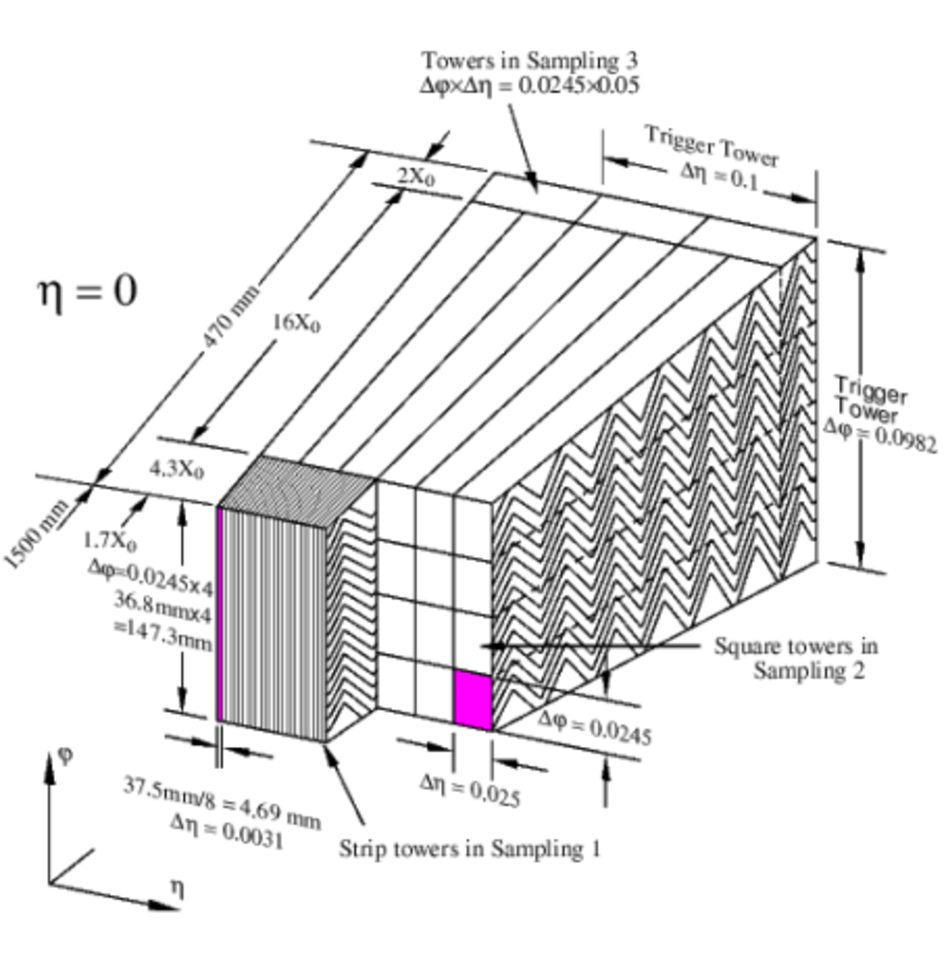
\includegraphics[width=0.6\textwidth]{ATLASDetector/images/LArg_accordion.pdf}	
	\caption{A depiction of a section of the LAr calorimeter.  The accordion structure of the towers is visible, as well as the three sampling layers. 	\label{fig:lar}}
\end{center}
\end{figure}


A notable feature of the EM calorimeter is the accordion geometry, which has several key characteristics.  First, 
the geometry enables complete coverage in $\phi$ without azimuthal cracks.  Second, the LAr sampling layer between 
lead layers is constant throughout the calorimeter barrel.  Third, a particle traveling through the calorimeter will generate approximately 
the same number of sampling instances (i.e. measurements) regardless of the direction in which it 
travels.  These pieces add up to a very uniform coverage of electromagnetic calorimetry.  The calorimeter consists of two 
major parts, the barrel and the endcaps; the barrel measures particles with $|\eta|<$1.475 
and the endcaps measure particles with 1.375$<|\eta|<$3.2.  The transverse segmentation of the calorimeter
is $\Delta\eta \times \Delta\phi<$0.03$\times$ 0.03 over the pseudorapidity region $|\eta|<$2.5,  
to allow for the particle identification and energy resolution needed \cite{cal_tdr}, while the 
calorimeter is up to 24 radiation lengths thick to minimize punch-through.

The performance requirement for the energy resolution of the EM calorimeter is 
$\sigma_E/E=\frac{10\%}{\sqrt{E}}+$0.7\%, which has the nice feature that the resolution improves
as the energy of an electromagnetic jet increases.
A crucial part of reaching this resolution is precisely understanding the shape of the readout pulse.  The traversing particle 
produces an electromagnetic shower where the drift time of the particles in the shower cause a readout pulse that is 
roughly triangular in shape and typically 400 ns long.  This pulse is shaped by the readout electronics and the 
signal shape is simulated with Monte Carlo and calibrated using precisely known test pulses deposited into the readout chain.  
However, as detailed below, the presence of multiple interactions per bunch crossing, known as pileup, has 
a significant effect in the calorimeters and is an important task for understanding jet energy.

%http://cds.cern.ch/record/1478440/files/ATL-TILECAL-PROC-2012-008.pdf
%http://arxiv.org/pdf/1305.0550v1.pdf
%http://cds.cern.ch/record/1393742/files/CERN-THESIS-2011-144.pdf
\subsubsection{Hadronic Calorimeter} 
\label{sec:h_cal}
Like the EM calorimeter, the hadronic calorimeter was designed with an eye toward Higgs discovery, that it would
have the resolution needed to find Higgs decays to $b\bar{b}$ and $\tau\tau$ pairs.  This is important and complementary
to the EM calorimeter because, although the most sensitive decay channels of the Higgs are to photons and electrons,
the decay modes with the highest branching fractions ($b\bar{b}$ and a large subset of $W^+W^-$) are hadronic.
For the physics in this thesis, with three $b$-jets in the final state, the hadronic calorimeter does the crucial
jet energy detection and measurement. 

Accurate measurement of hadronic energy is crucial for accurately reconstructing $b$-jets, and the hadronic calorimeter also measures the 
energy from hadrons, jets, taus and allows for a measurement of missing transverse energy.  The hadronic calorimeter 
is a sampling calorimeter, nicknamed the tile calorimeter because of its composition of scintillating tiles (active material) 
interleaved with steel plates (showering material) in the barrel.  When a strongly-interacting particle hits the steel it creates a 
spray of particles, called a shower, which then enters the scintillator and creates a light signal that is 
proportional to the energy .  This process repeats until the full energy of the original particle is measured, and 
usually the calorimeter cells are reconstructed into an object called a jet which aims to cluster the energy together in 
a way that accurately represents the energy of the original particle.  Much more on hadronic jet reconstruction will follow in Section~\ref{sec:jet_reco}.

The hadronic calorimeter is partitioned into four major subsections, two barrel sections and two extended barrel sections, allowing 
for measurements out to $|\eta|<$1.7.  In the forward regions, hadronic coverage is provided by the liquid argon system and the high-density forward calorimeter \cite{cal_tdr}. In order to stop all remaining particles from the collision, 
with the notable exception of muons, the hadronic calorimeter is about 7.4 radiation lengths ($\lambda$) thick.

\begin{figure}
	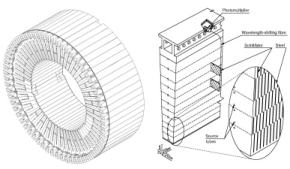
\includegraphics[width=0.8\textwidth]{ATLASDetector/images/tile_cal.pdf}
	\caption{A depiction of the scintillator-and-steel hadronic calorimeter, also known as the tile calorimeter, and a close-up view of one of its cells.	\label{fig:tile_cal}}
\end{figure}


%http://iopscience.iop.org/1742-6596/331/2/022024/pdf/1742-6596_331_2_022024.pdf

\subsection{Muon System}
\label{sec:ms}
Muons are very similar to electrons in their interactions, but they are about 200 times heavier and as a 
result, they can travel largely unaffected through the inner detector and calorimeters and emerge in the outer layers of 
the detector, where the muon system is situated to make dedicated measurements of muons.  The muon system is 
often used in conjunction with the tracking of the inner detector, since a muon interacts electromagnetically and would be 
expected to create a track in both systems.  These tracks in the two different subsystems can then be combined 
into a single measurement of the $p_T$ of the muon.  Muons are largely not used 
in this analysis, so we will be brief in explaining the muon system, although they may play an 
important role in the future since muons can be used to help trigger on and identify $b$-jets.


The ATLAS muon system is composed of four different detector systems located within and around an air-core toroid 
magnet with a field of 1 Tesla.  Precision tracking in the barrel is done by Monitored Drift Tubes (
MDT) and in the endcap by Cathode Strip Chambers (CSC).  Quick-readout triggering is done in 
the barrel by Resistive Plate Chambers (RPC) and in the endcap by Thin Gap Chambers (TGC).   
The system is designed to measure the $p_T$ of muons with $p_T>$
3 GeV, with 3\% resolution up to $p_T<$250 GeV and 10\% resolution up to 1TeV.  



%%% ATLAS detector figure
\begin{figure}
	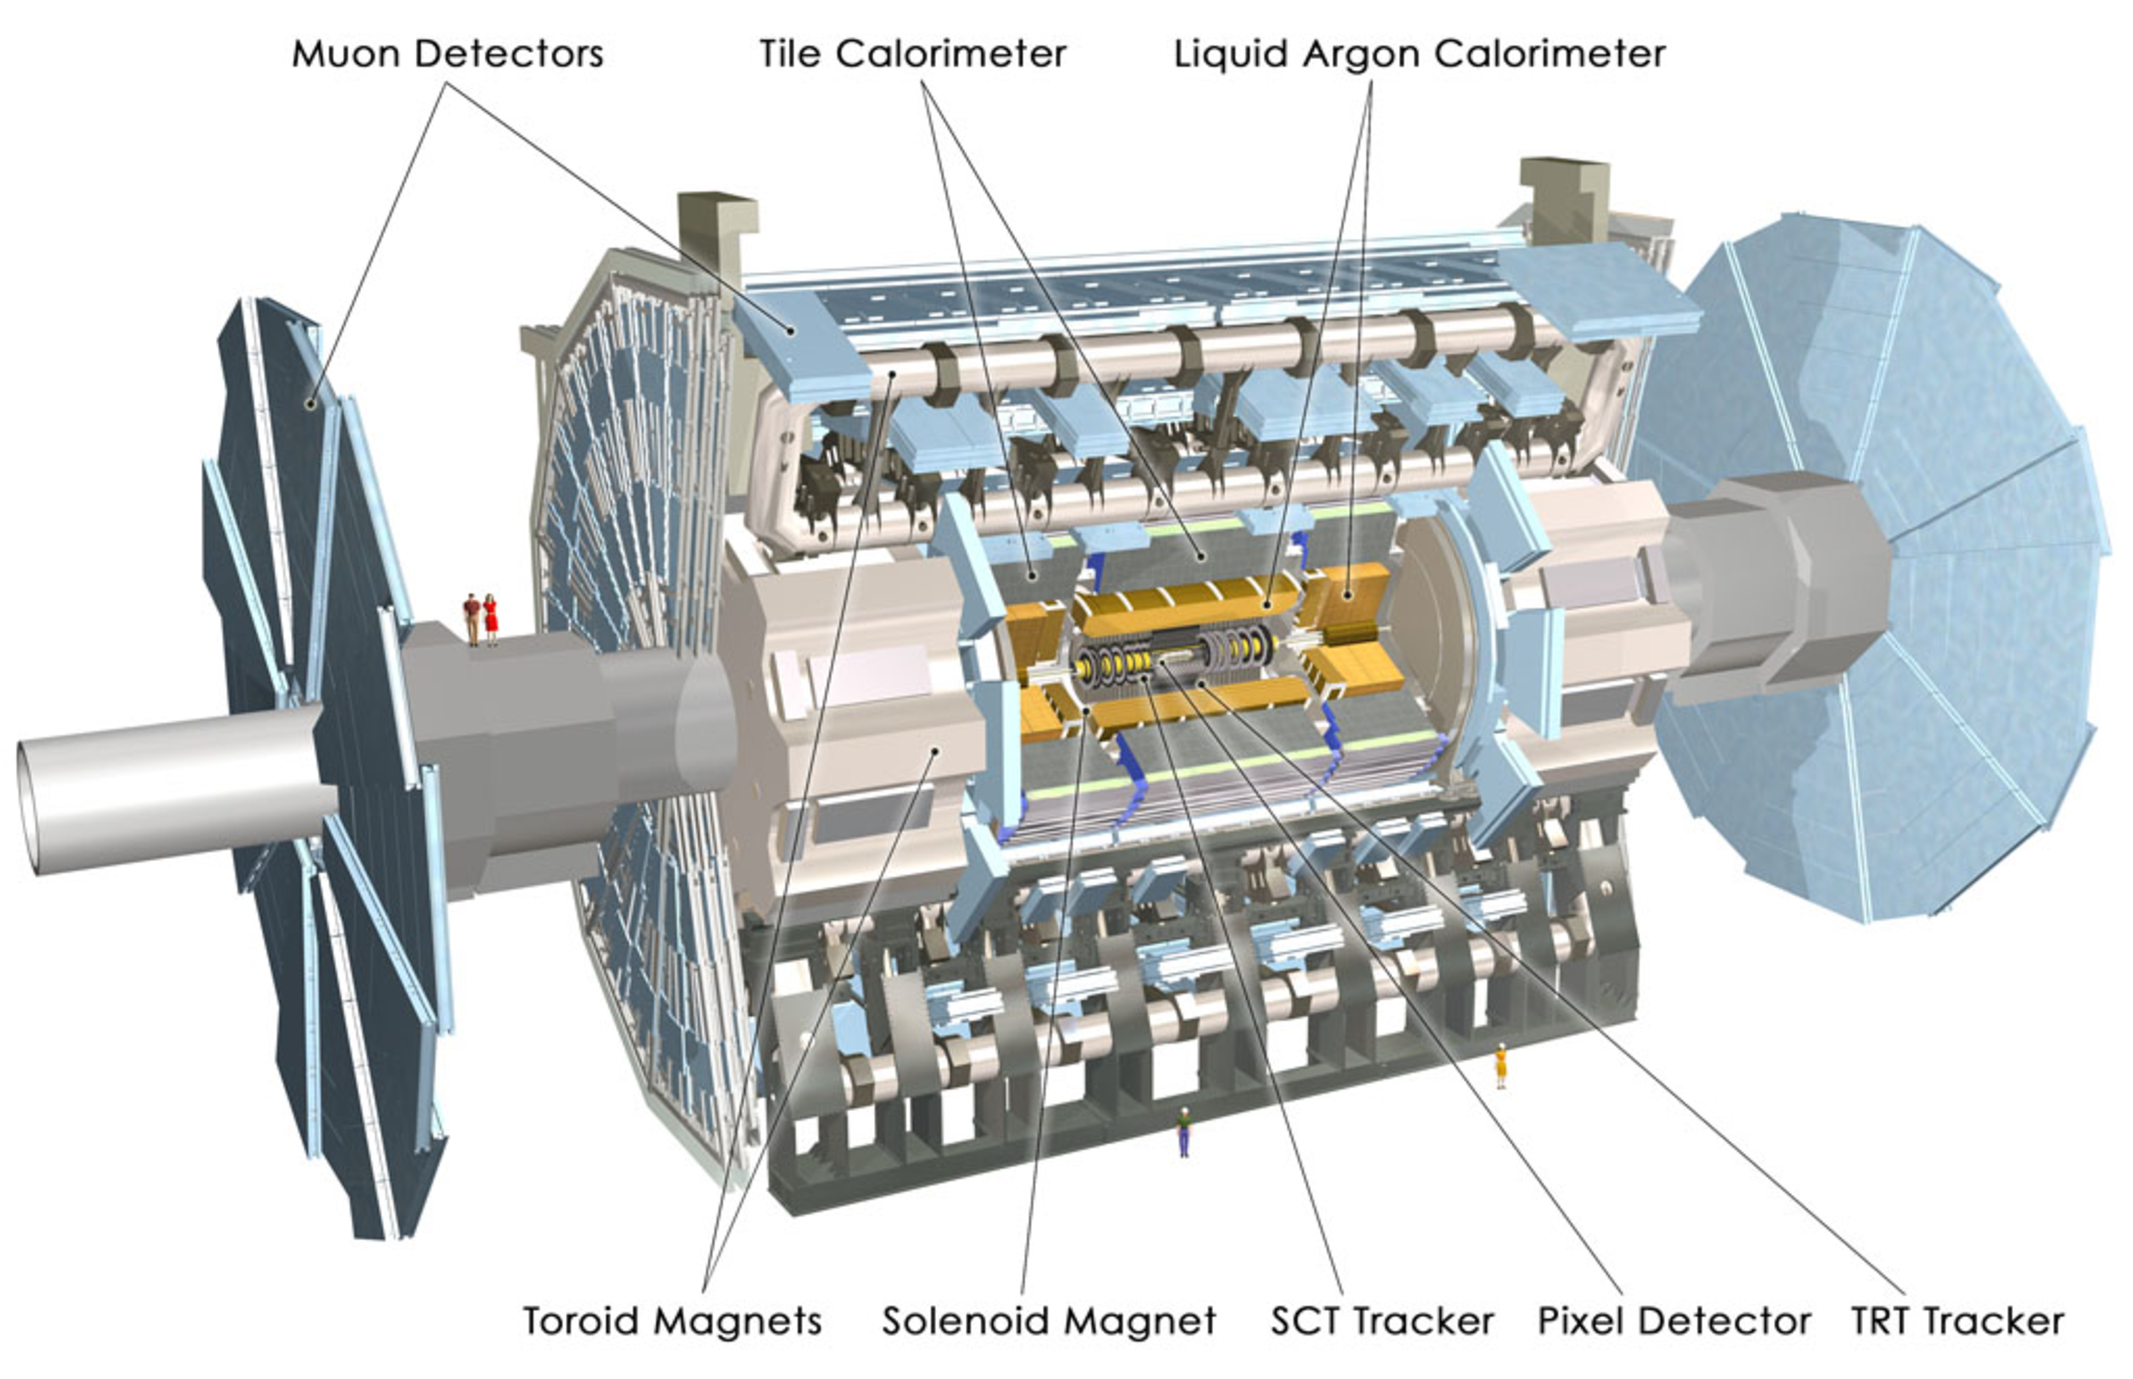
\includegraphics[width=\textwidth]{ATLASDetector/images/AtlasDetectorLabeled.pdf}	\caption{A diagram of the ATLAS detector as a whole, with major subsystems labeled.  A couple of human figures are shown standing on and near the detector, for scale. \label{fig:detector}}
\end{figure}

%http://www.slac.stanford.edu/econf/C0303241/proc/pres/502.PDF
%https://cds.cern.ch/record/1267390/files/ATL-DAQ-SLIDE-2010-087.pdf
\section{The ATLAS Trigger and Data Processing}
\label{sec:atlas_trig}
Although the LHC delivers 20 million bunch crossings per second to the ATLAS detector, the detector does not have 
the capacity in either storage space or readout bandwidth to record all these collisions.  The trigger has the task 
of selecting the most interesting 200 or so events per second, which are then fully reconstructed and recorded.  
The trigger is a three-layer system, with a first level (L1) implemented solely in hardware
, a second level (L2) that reconstructs ``regions of interest'' (RoIs) with special fast 
algorithms, and an event filter (EF) that reconstructs the full event with offline algorithms.  L2 and 
EF together are called the high level trigger, or HLT.

In what follows, we will make use of the following terminology in explaining the structure and performance of the trigger:

\begin{itemize}
	\item trigger object: the signature left by a particle in the detector, once it has been reconstructed and identified.  Examples include electrons, muons, photons, and jets.
	\item trigger item: one or more trigger objects that define whether an event passes a particular level (L1, L2, EF)
	\item threshold: the minimum momentum or energy required in order for a trigger object to be accepted.
	\item trigger accept: when all the requirements for a particular trigger level are met, and the event gets promoted to the next level.

	\item trigger chain: a set of L1, L2 and EF trigger items (also called simply a trigger).
	\item trigger menu: the set of all L1, L2 and EF trigger items, which collectively define which events will be written to disk.
	\item trigger prescale: a set reduction factor, so that a trigger can be maintained with low thresholds while not exceeding rate limits.  For example, for a trigger with a prescale of 10, only 1 in 10 events passing the trigger get written to disk.
\end{itemize}
 

The trigger has a step-type structure, where progressively smaller numbers of events are processed with progressively more 
detailed and computationally intensive algorithms.  Many physics analyses look for signatures that have more than one physics object in 
them (for instance, multiple electrons, or a lepton plus jets), so multiple physics objects are often 
required in a single trigger.  There are also single-item triggers, although typically these have higher thresholds 
than triggers that look for multiple objects.  If all of the objects in a given trigger item are seen
, the event is accepted for the current level and the event moves forward in the data collection process.  
This process repeats three times, once for each of the levels of the trigger--only those events which 
pass L1 move onto L2, those which pass L2 move on to EF, and those that pass EF 
are written to disk.   As the machine settings for the LHC changed over the course of 2012, resulting 
in different conditions for data-taking, the trigger menu was adjusted periodically to keep rates under control (
in practice, this generally means either raising thresholds or adding prescales).  


Groups of trigger chains that share common features are grouped together into trigger streams, where the primary trigger streams 
are JetTauEtMiss, EGamma, MinBias, and CosmicCalo.  The end result of this process is approximately 200 events 
per second (320 GB/s of data) being written to disk; the trigger rates and latency 
information can be found in Table \ref{tab:trigger_stats}.

  

% https://cds.cern.ch/record/1181075/files/05446486.pdf
\begin{table}
\begin{tabular}{c | c | c | c}
Trigger Level & Rate in Hz  & Latency  & Data Rate\\  \hline
None (Event rate) & 20 MHz  & no decision applied yet & 1600 TB/s \\
L1  & 75 kHz  &  $\sim$ 1$\mu s$  & 120 GB/s\\
L2  & 3 kHz    & $\sim$ 10 ms & 5 GB/s \\
EF  &  200 Hz  & $\sim$ 1 s & 320 MB/s \\
\end{tabular}
\end{table}
\label{tab:trigger_stats}


Of particular interest to this analysis are the jet thresholds and b-tagging applied in the trigger.  This 
will be outlined in greater detail in a later section, but we will introduce the ideas here.  As 
only 200 events per second get written to disk, the bandwidth has to be carefully allocated across triggers, 
and it is very expensive to keep a trigger that allows high rates of events to be written to data
.  In an analysis such as this one, the physics objects coming from the signal (b-jets 
from a Higgs decay) are generally higher in p$_T$ than the background (continuum QCD processes
) so one way to keep event rates reasonable in the face of rising luminosity is to place higher p$_T$ 
thresholds on the jets that fire the trigger.   

The thresholds increase with each trigger level, as more information is read out of the detector, so that 
a jet which is reconstructed with 145 GeV of p$_T$ at L1 
might be required to have 155 GeV at EF in order to pass the full trigger.  Once the event 
is written to disk, it is subject to the full offline reconstruction and calibration so that the final p$_T$ 
of the jet might not be exactly the number measured at the trigger EF.  There is therefore a range 
of p$_T$ values, called the turn-on curve, where the trigger goes from rejecting 
all events to accepting all events.  Within the turn-on curve even a small change in the p$_T$
of a jet can have a dramatic difference in whether the jet fires a trigger accept, so this 
instability is mitigated by placing p$_T$ cuts on the trigger jets that require that their respective p$_T$ 
values are above the turn-on curve.  

The ATLAS trigger also allows for b-tagging of jets at L2 and EF.  For analyses that have 
b-jets in the final state, b-tagging in the trigger provides a tool for keeping rates 
low without pushing up jet p$_T$ thresholds.  B-tagging in the trigger introduces several challenges
, though.  First, the online b-tagging algorithms have less time and information than the offline algorithms
.  Second, a jet that passes an L2 b-tag will not necessarily pass an EF b-
tag, and vice versa, so more work is required in understanding the correlations between tags at different trigger 
levels.  









% Activate the following line by filling in the right side. If for example the name of the root file is Main.tex, write
% "...root = Main.tex" if the chapter file is in the same directory, and "...root = ../Main.tex" if the chapter is in a subdirectory.
 
%!TEX root =  ../Thesis.tex

\chapter[Reconstruction and Performance]{Event Reconstruction and Performance}
Once the physics data has been created by the LHC, detected by the ATLAS detector, and written to 
disk by the ATLAS trigger and data acquisition system, it is reconstructed into physics events.  This process has 
many interacting steps.  First, hits in the inner detector are algorithmically combined into tracks, which approximate the 
trajectory of charged particles, while energy clusters in the calorimeters are grouped together into jets, which seek to 
capture the energy of the particle that originated the jet.  

Higher-order quantities and corrections also come into play.  Two of the most important are the calibration and removal of 
pileup, other lower-energy interactions from the same or adjacent bunch crossings, and $b$-tagging
, which primarily uses tracks to identify jets that are likely originated by $b$-quarks.  Additionally, 
there are jet energy corrections that account for jet radiation that could by lost by the jet clustering algorithms, 
$b$-tagging efficiency corrections, and uncertainties on the total luminosity collected. 



\section{Track Reconstruction}
\label{sec:trk_reco}
%https://twiki.cern.ch/twiki/pub/AtlasPublic/EventDisplayStandAlone/2012_highPileup.png
Track reconstruction takes place in the inner detector and allows crucial measurements such as the primary and secondary vertices.  
When a charged particle traverses the layers of the inner detector, it leaves typically 8-11 hits in 
silicon (counting one double-sided layer of SCT silicon as capable of seeing 2 hits) and about 
35 in the TRT.  The track reconstruction algorithm, as detailed in section~\ref{sec:id_perf}, 
starts by identifying track seeds and then iterating through a Kalman filter algorithm, projecting out to further tracking layers 
and then checking for hits along the hypothesized trajectory of the particle.  

Track reconstruction performance can be impacted by pileup, as more pileup (and hence more tracking hits) creates 
more opportunities for incorrectly assigned hits and fake tracks from random hits being falsely associated with each other.  A 
second effect of pileup on tracking is indirect: the detector as a whole, and the silicon detectors in 
particular, undergo radiation damage as luminosity accrues.  Radiation damage in silicon detectors manifests 
itself as rising leakage current, which makes channels prone to more noise hits unless the thresholds are raised (
but higher thresholds lowers the efficiency for legitimate hits).  As time goes on, the tracking quality can can 
be affected by the extra noise hits and/or higher thresholds.

\begin{figure}
	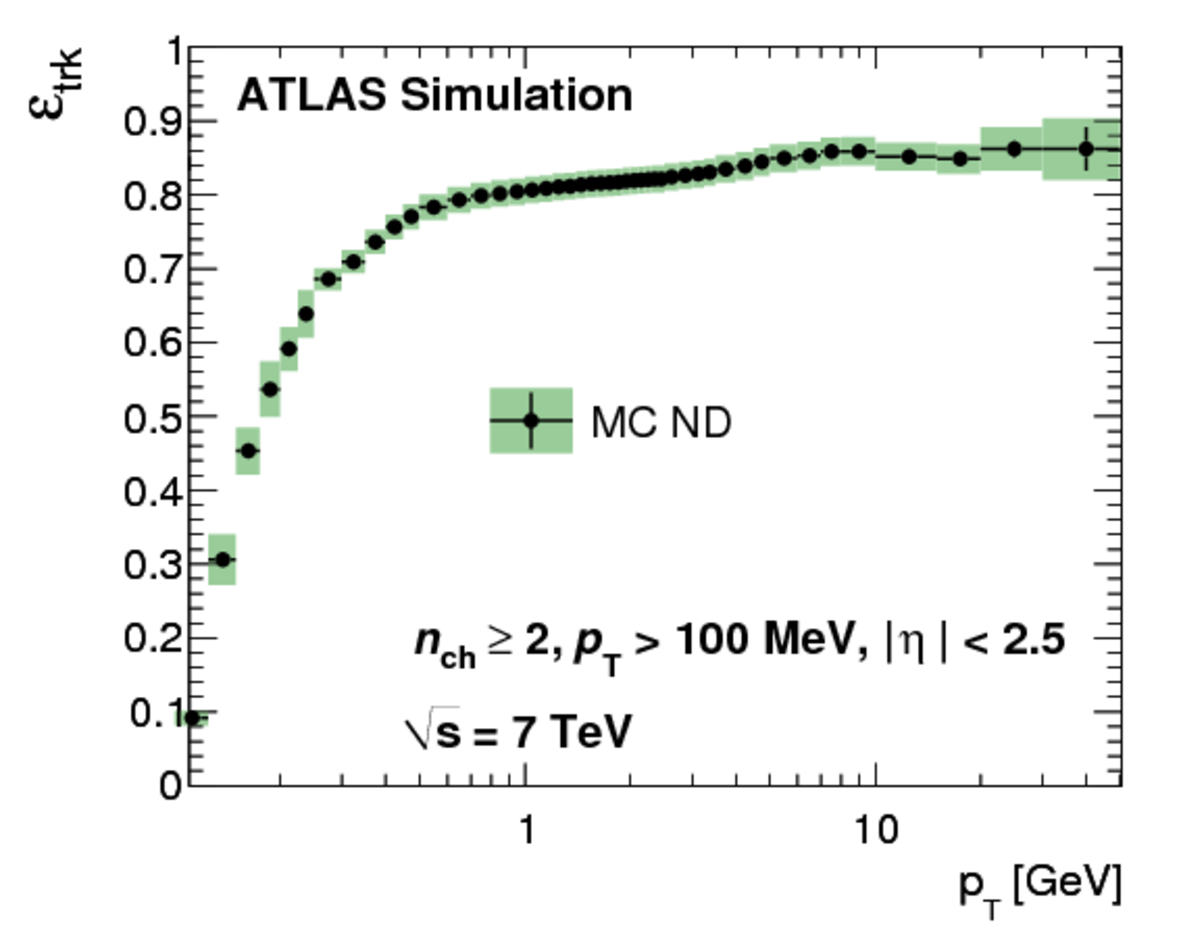
\includegraphics[width=0.5\textwidth]{ReconstructionPerformance/images/track_perf1.pdf}
	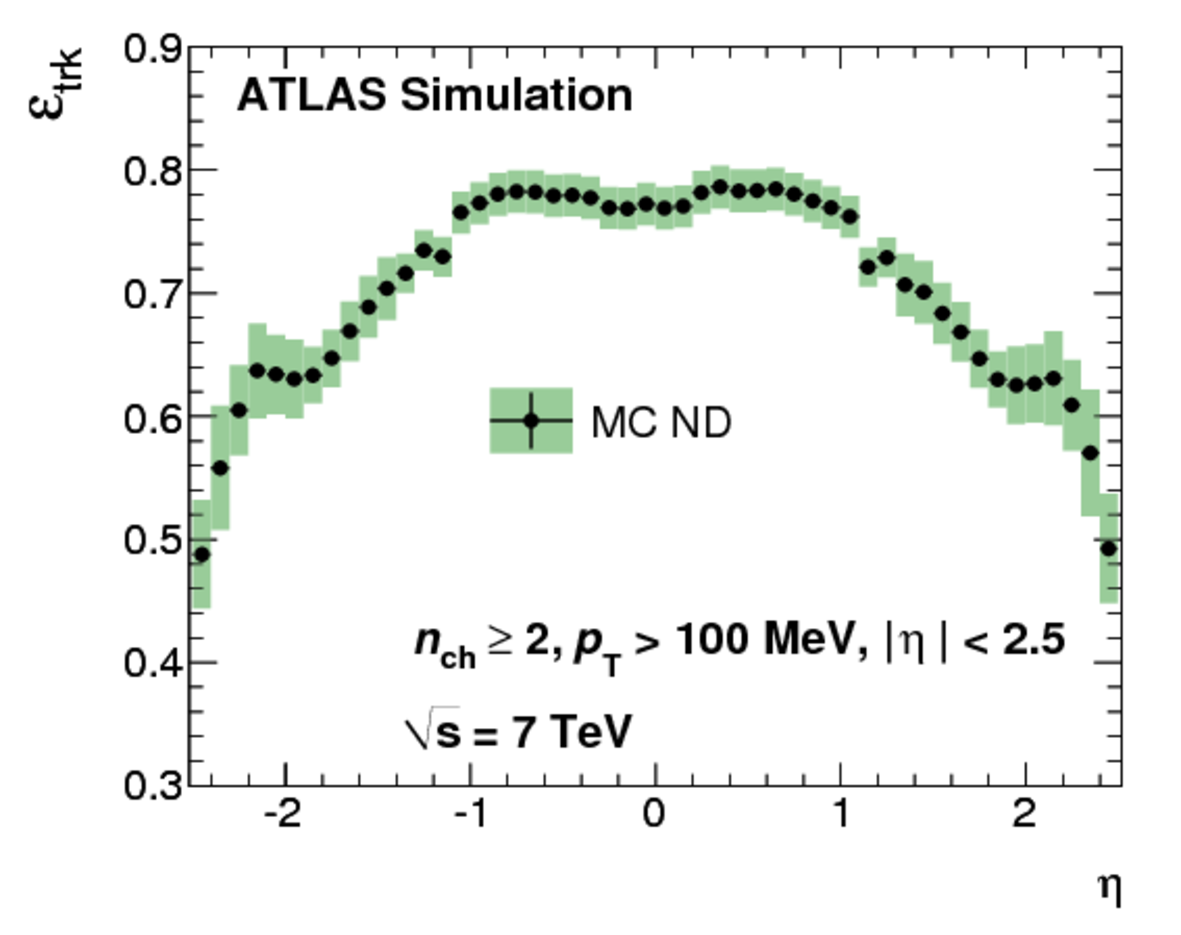
\includegraphics[width=0.5\textwidth]{ReconstructionPerformance/images/track_perf2.pdf}
	\label{fig:track_perfA}  
	\caption{The efficiency of the track reconstruction, projected in $p_T$ and $\eta$, as computed in Monte Carlo.}
\end{figure}



\begin{figure}
	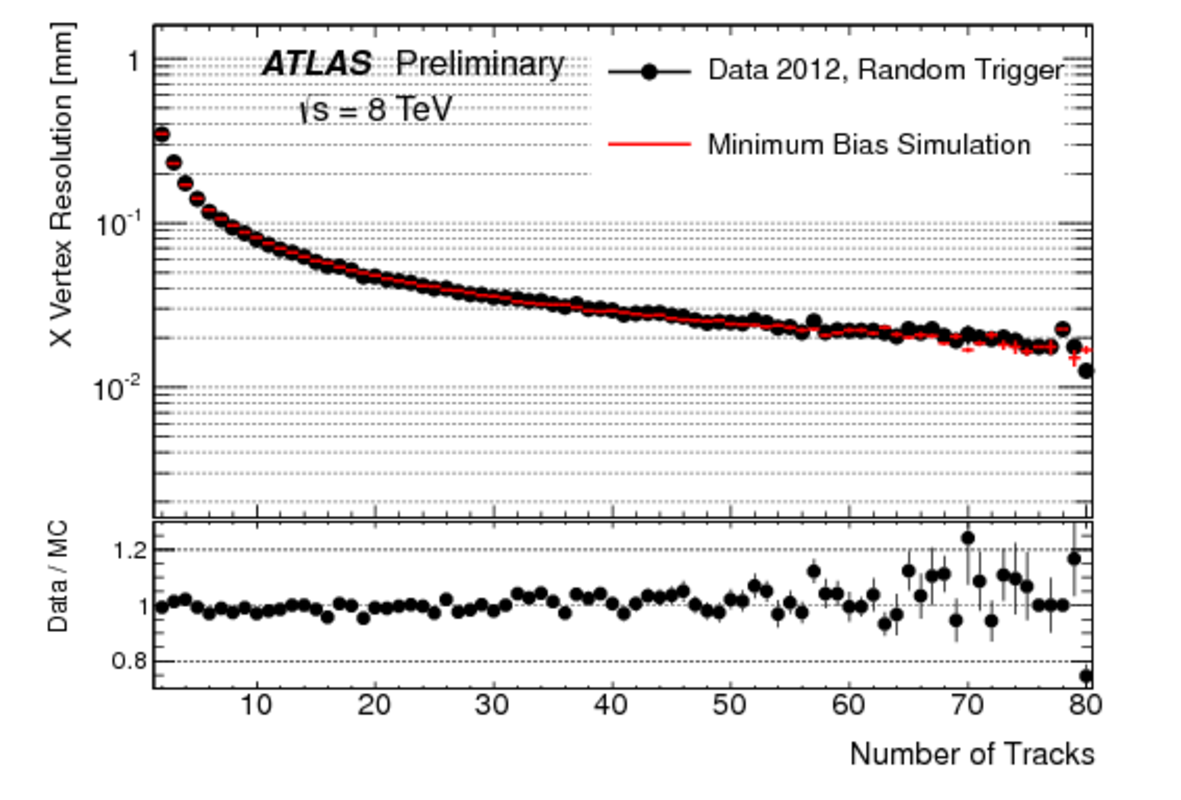
\includegraphics[width=0.5\textwidth]{ReconstructionPerformance/images/track_perf3.pdf}
	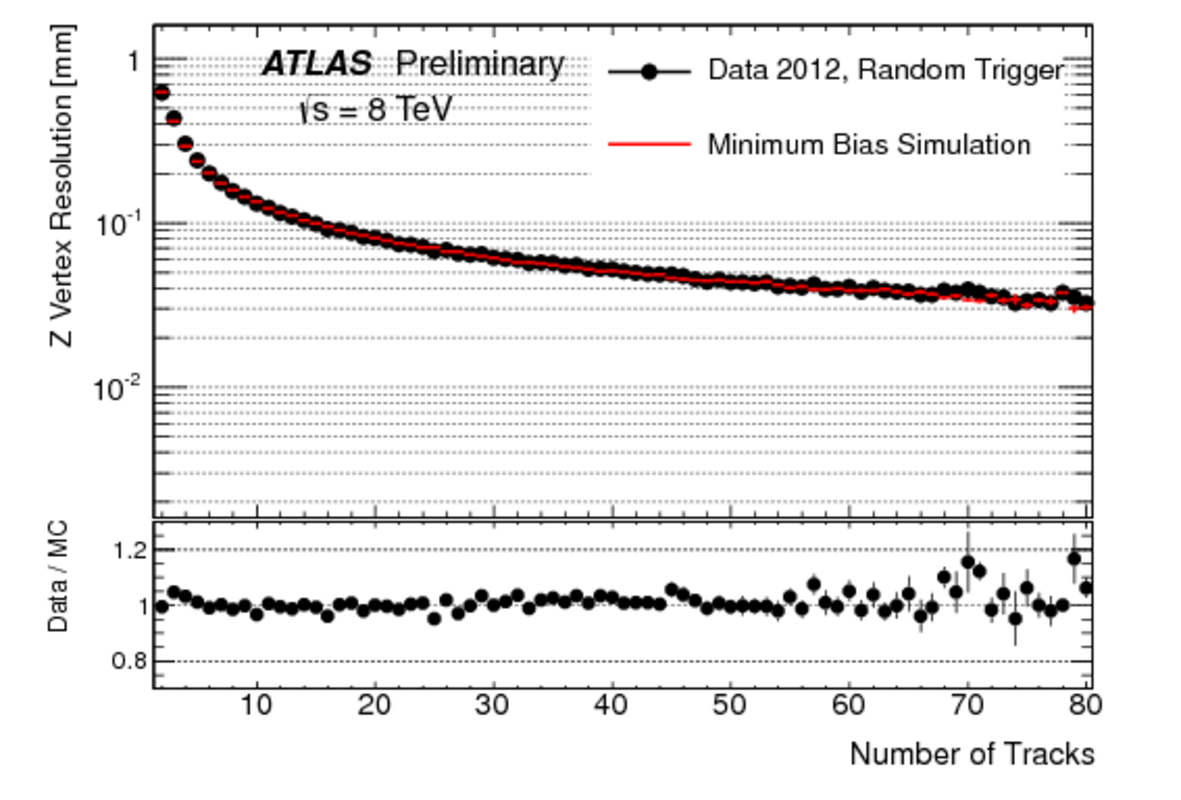
\includegraphics[width=0.5\textwidth]{ReconstructionPerformance/images/track_perf4.pdf}
	\label{fig:track_perfB}  
	\caption{The track resolution in mm the $x$ and $z$ directions, comparing minimum bias simulation to data taken with a random trigger.}
\end{figure}

Good tracking performance enters this analysis most directly in its impact on the tagging of $b$-jets, as detailed in Section~\ref{sec:b-tag}.  Well-reconstructed tracks allow for the identification of a secondary vertex, which is one of the fundamental features of the ATLAS $b$-jet tagging algorithms.

% http://www.slac.stanford.edu/cgi-wrap/getdoc/slac-pub-5671.pdf
% http://www.quantumdiaries.org/2011/06/10/to-b-or-not-to-bbar-b-tagging-via-track-counting/
% http://dorigo.wordpress.com/2007/05/15/b-hadron-lifetimes-part-2/

% http://iopscience.iop.org/1742-6596/119/3/032014/pdf/1742-6596_119_3_032014.pdf
\subsubsection{Inner Detector Performance and Tracking}
\label{sec:id_perf}
Measurements from the pixel, SCT and TRT are combined in the track reconstruction.  There is a broad range 
of properties that tracks might have, so the inner detector has to be able to measure tracks with p$_T$
 ranging from 150 MeV to 30 GeV or more.   

The main track reconstruction algorithm used at ATLAS is a version of the Kalman filter algorithm.  The track reconstruction 
begins with track seeds, which are collections of a few hits in the pixel subsystem that could plausibly be 
parts of tracks.  The advantage of starting with seeds, rather than attempting to find an entire track at 
once, is that seeds allow flexibility at the beginning of the search (when the track trajectory is the 
least known) while keeping computational costs down.  Once a seed has been identified, the Kalman fitter (
as the ATLAS algorithm is called) projects where the next hit would be if there is truly a track 
present, and then looks for the presence of a hit at the predicted location in the next tracker layer
.  If a hit is found there, the predicted trajectory of the particle may be refined and the next 
hit is predicted and sought, until all the detector layers have been traversed. If there is no hit 
present where one is predicted, the Kalman fitter can project two layers further, to allow for the possibility 
of a hole where the particle did not leave a hit for some reason. 

In high-pileup environments, the inner detector occupancy can be high which can make for two tracks that 
overlap, leaving a hit in the same place which must then be allocated to one or the other.  
Dedicated ambiguity solving is implemented as a second stage in the track reconstruction, where the two candidate tracks are 
scored against each other via a reward/penalty scheme.  A good $\chi^2/DOF$ 
score is rewarded, a track with many holes on track or a low $\chi^2/DOF$ 
is penalized, with subdetector-specific weighting favoring the higher-precision silicon over the the lower-precision TRT. 



%http://arxiv.org/pdf/0802.1189.pdf
%http://iopscience.iop.org/1126-6708/2008/04/063/pdf/1126-6708_2008_04_063.pdf
\section{Jet Reconstruction}
\label{sec:jet_reco}
Because of asymptotic freedom of QCD, quarks and gluons do not remain standalone particles once they're produced
, but instead they hadronize and shower as they travel through the detector.  Hypothetically, all the particles of 
the shower can be added back up to approximate the energy, momentum, and angle of the original quark 
or gluon.  Jet reconstruction is the process of assembling calorimeter deposits together into a physics object, called a 
jet, that ideally will do a good job of representing the characteristics ($p_T$, energy, 
flavor) of the quark or gluon that originated the jet.  There are a number of clustering algorithms for 
assembling the calorimeter cells, and post-processing steps for improving the performance of jets in analyses--pileup 
subtraction, energy calibrations, grooming, and trimming, to name a few.  

The default jet clustering algorithm in ATLAS is the anti-$k_t$ algorithm \cite{antikt}
with a distance parameter of 0.4.  Roughly summarized, this algorithm starts with a calorimeter cell that 
has an energy deposit at least $4\sigma$ higher in energy than the ambient and pileup noise, 
and then the surrounding cells with at least $2\sigma$ more energy than noise are grouped into 
the jet in a way that prioritizes high energy over close proximity.  The result is that soft deposits get 
clustered in with hard deposits, rather than clustering amongst themselves.  The distance parameter of 0.4 is 
a cutoff as to how far away from the seed in $\eta-\phi$ space to look for 
additional deposits.   Jets below 20 GeV or so can be difficult to distinguish from noise, so in practice, a lower limit on 
the $p_T$ (in the case of this analysis, 25 GeV) is often applied.  

A critical feature of this algorithm, or any jet algorithm, is that it be infrared and collinear safe
.  In technical terms, that means that when additional `ghost' particles with infinitesimally small energy or infinitesimally 
close radius are added to the area in and around the jet, the properties of the resulting jet do 
not change.  In practical terms, it means that the jet is stable to small perturbations, so that 
the presence or absence of low-energy nearby radiation (which can be difficult or impossible to distinguish from 
calorimeter noise) or the precise direction of energy that is highly collinear with the jet itself (the direction 
of this energy can be prone to resolution uncertainties) do not affect the jet properties.  Critically, the 
anti-$k_t$ algorithm is both infrared and collinear safe.







%https://twiki.cern.ch/twiki/bin/view/AtlasPublic/LuminosityPublicResults#Data_Taking_Efficiency_and_Pileu

\section{Pileup Calibration and Removal}
\label{sec:pileup}
All the detector subsystems are affected by the presence of pileup, which are collisions other than the hard scatter 
collision.  As the LHC delivers higher luminosity for a given number of proton bunches, the luminosity increase comes 
at the price of many interactions per bunch crossing, and these softer interactions create extra activity in the detector 
that tends to make events noisier and more challenging to reconstruct accurately.  In 2012, the mean number of 
interactions per crossing ranged from about 10 up to about 40.  

The inner detector and tracking provide an important tool for understanding in-time pileup.  In-time pileup 
is additional soft interactions in the same bunch crossing as the hard scatter.  The tracking allows primary vertex reconstruction 
with a resolution fine enough in z$_0$, for the pixels typically $z_0\sin\theta$, 
to resolve separate primary vertices from each other \cite{pileup_tracks}.   The calorimeters cannot resolve individual primary vertices with such precision, 
though, so a constant struggle in ATLAS is to measure the calorimeter deposits that come from pileup interactions, 
and where possible to apply corrections that subtract away pileup contributions to jets from the hard scatter.  On average
, each additional pileup vertex in an event adds 370(850) \cite{pileup} MeV to the p$_T$ of a jet reconstructed with the Anti-kT algorithm with R=0.4(0.6).

In addition to in-time pileup, the calorimeters are prone to out-of-time pileup where 
the signal in a given in event can be affected by the energy flow of previous collisions because of the 
calorimeter readout signal shapes.  Out-of-time pileup has the effect of adding an average of 60
(210) MeV to central jets, and decreasing the forward jets by 350(470) MeV.  


\begin{figure}
	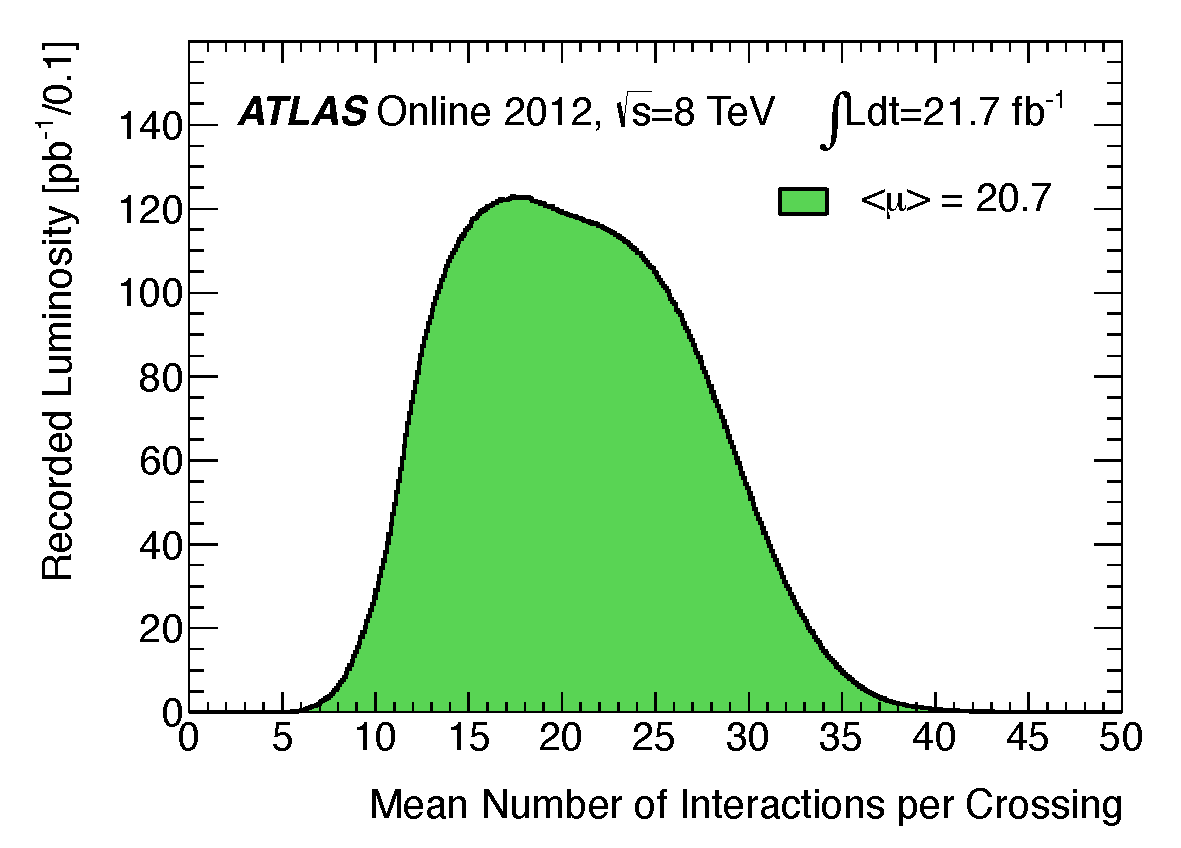
\includegraphics[width=0.8\textwidth]{ReconstructionPerformance/images/mu_2012-dec.pdf}
	\caption{A distribution of the mean number of interactions per crossing, also called $\mu$ seen in 2012 data-taking.  Larger $\mu$ values are characterized by more challenging reconstruction. 	\label{fig:mu_2012}  }
\end{figure}

% http://cds.cern.ch/record/1435196/files/ATLAS-CONF-2012-042.pdf
%http://iopscience.iop.org/1742-6596/119/3/032033/pdf/1742-6596_119_3_032033.pdf
\section{Primary Vertex Identification}
\label{sec:pv}
Both the hard scatter collision and pileup collisions produce charged tracks; once these tracks are reconstructed, they can 
be traced back to the interaction region of the ATLAS detector and used to figure out where collisions took place
.  Each time a group of tracks can be clustered together into a presumed collision, we refer to it 
as a primary vertex.  The reconstruction of primary vertices is one of the reasons that tracking resolution must be 
so precise; primary vertices are often separated by only a few mm so imprecisely measured tracks can cause unintended 
merging.  The consequence of mistakes in the primary vertex reconstruction can be physics objects that get grouped with the 
wrong primary vertex, and lead to incorrect event reconstruction and either signal loss or undesired background acceptance.

The reconstruction errors on the primary vertex are generally within 0.02 mm in the x/y directions 
(transverse to the beam direction) and 0.1 mm in the z direction (longitudinal to the  
beam) \cite{pileup_tracks}.   This resolution can be seen in Figure~\ref{fig:pileup_pv}, a 2012 
$Z\rightarrow\mu\mu$ event with 25 reconstructed primary vertices.



%-----------------------------------------------------------------------------
\begin{figure}
	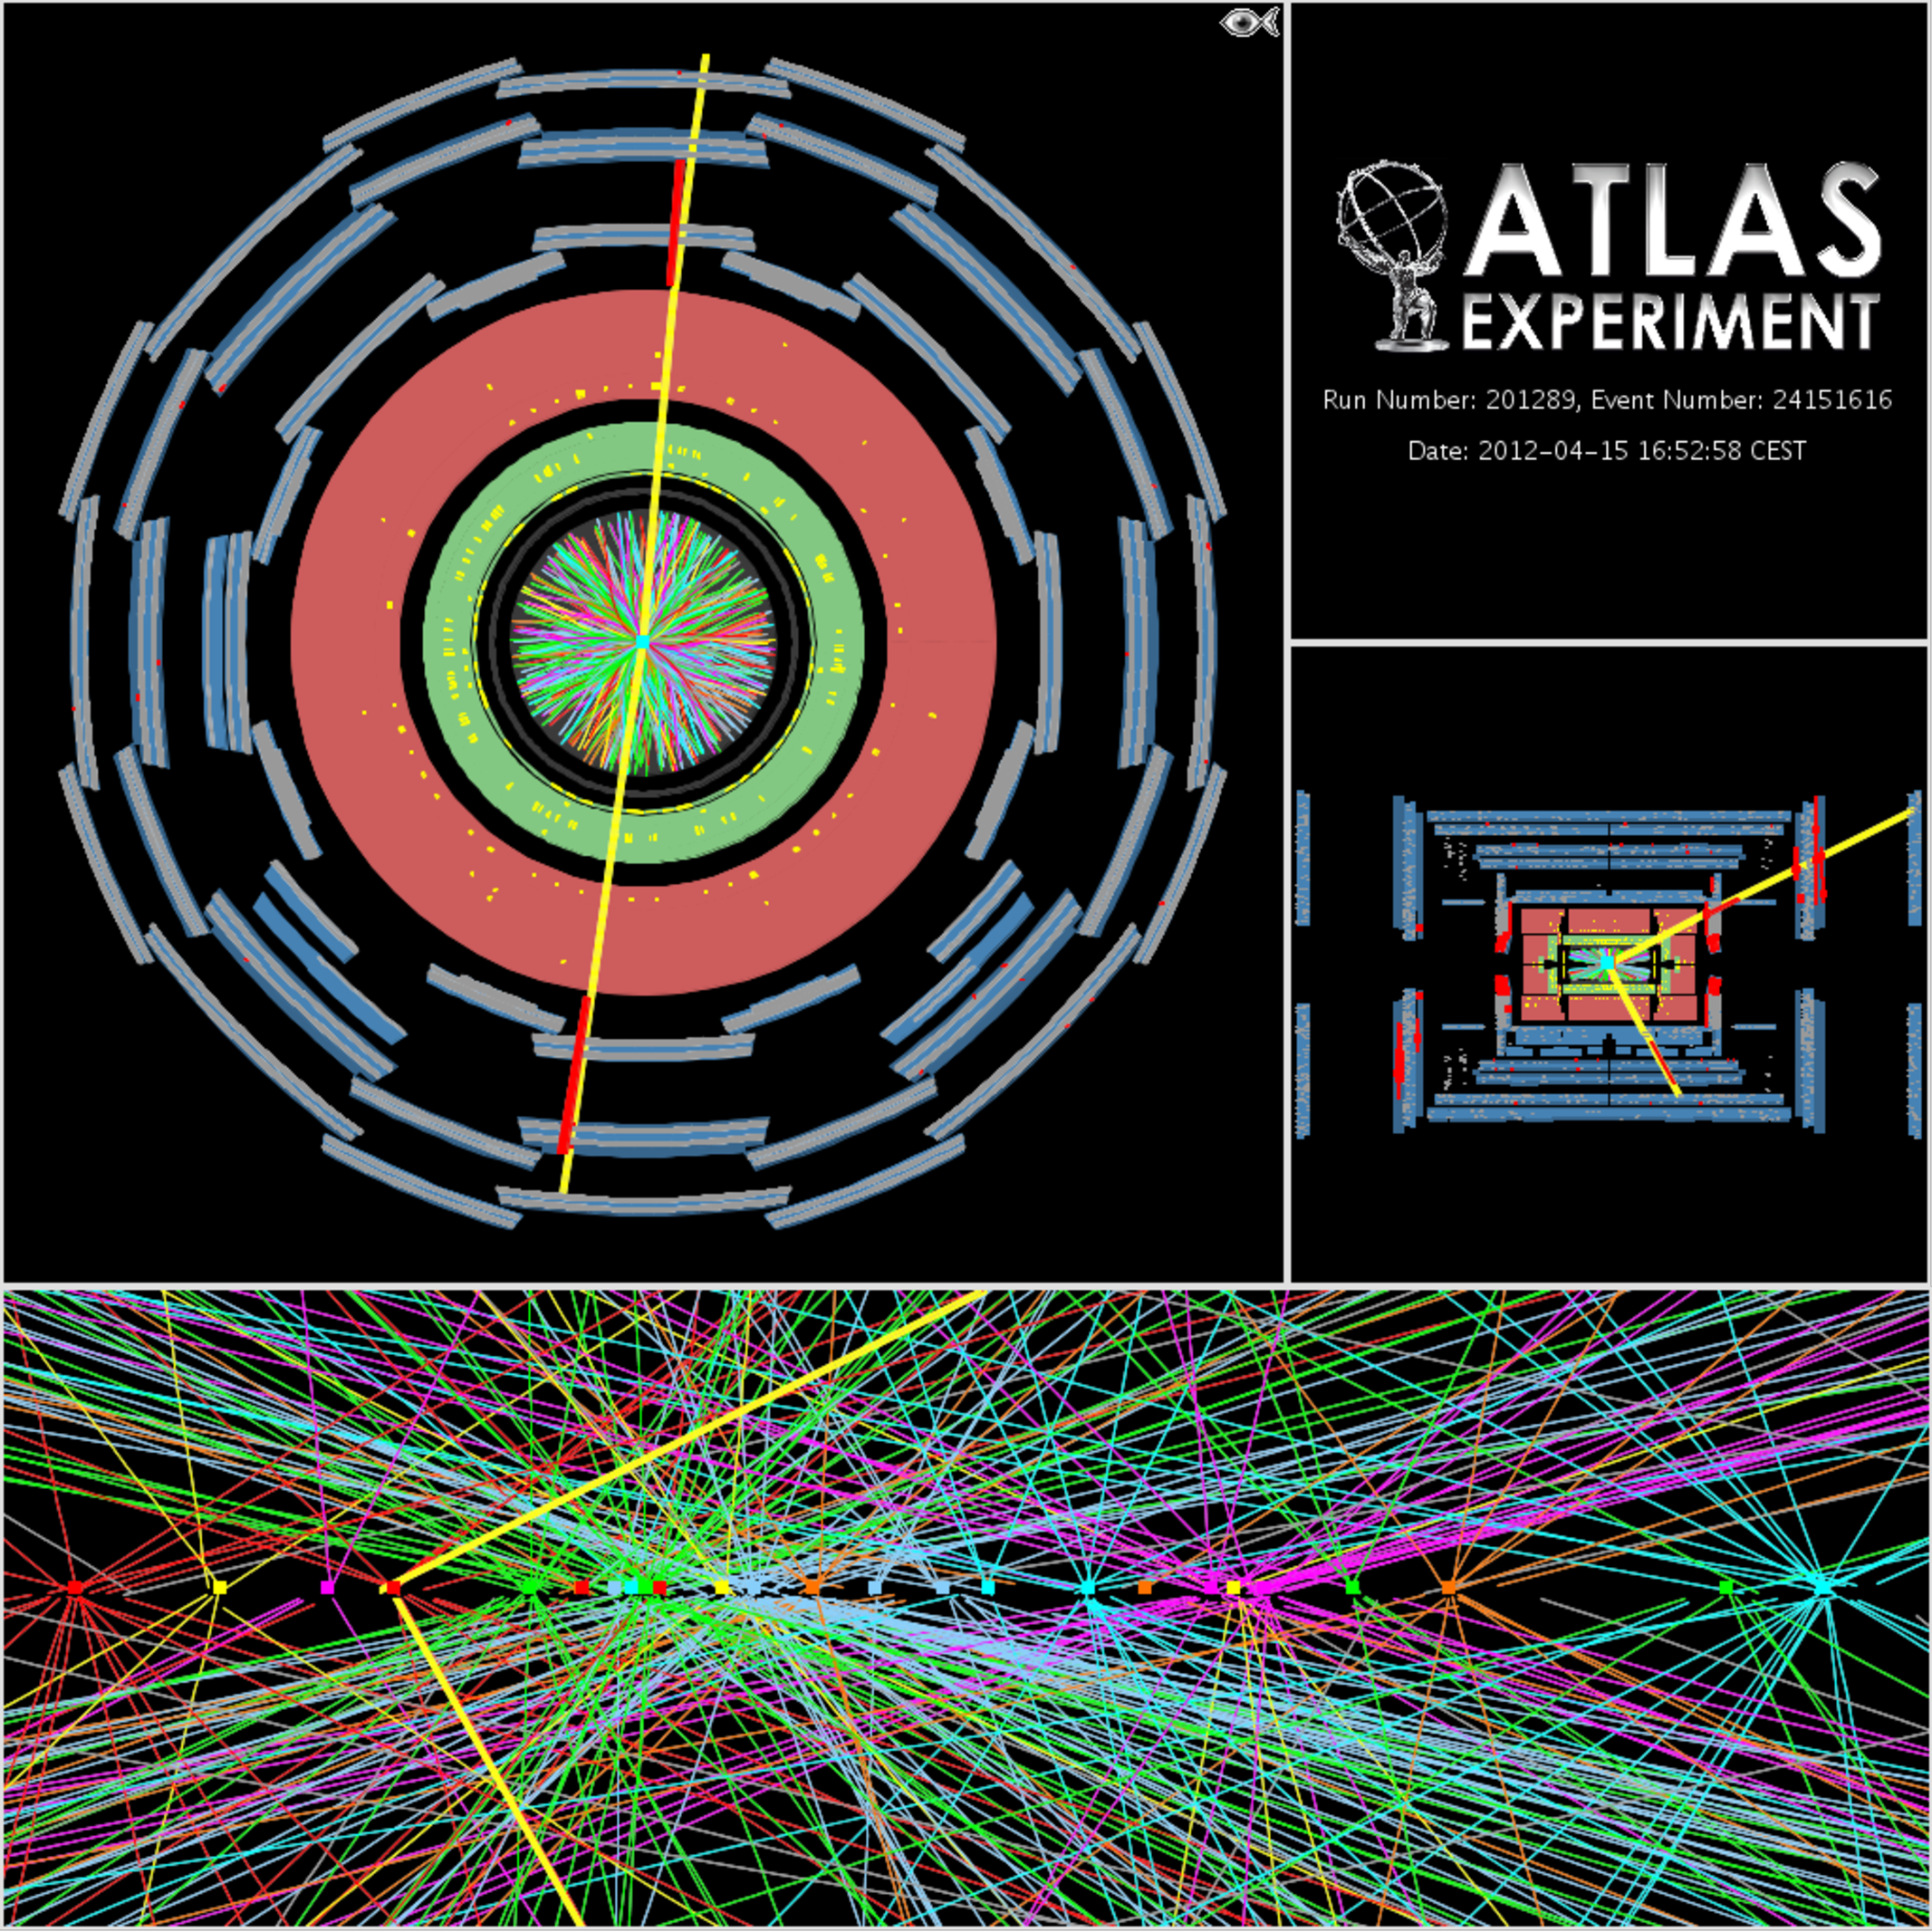
\includegraphics[width=0.8\textwidth]{ReconstructionPerformance/images/2012_highPileup.pdf}
	\caption{A data event taken in 2012, showing the occupancy typical of high pileup. 	\label{fig:pileup_pv}  }
\end{figure}
%-----------------------------------------------------------------------------


\section{$b$-Tagging}
\label{sec:b-tag}
B quarks typically have a lifetime of about 1ps
, and since they are often created in high-p$_T$ collisions or come from the decay 
of heavy particles, they can have considerable $p_T$ and travel a few millimeters before decaying
.  B-tagging algorithms typically look for evidence of secondary decay vertices that are displaced from the beamspot in 
the transverse direction.   



Another critical tool built on top of good tracking is $b$-tagging, or identifying jets that likely 
came from $b$-quarks.  A unique feature of $b$-quarks relative to other strongly interacting 
particles is the long lifetime of $b$-quarks, which means that they can travel a few mm 
out from the primary vertex before decaying.  This feature of $b$-jets means they can be identified 
by the presence of one or more kinematic characteristics:


%-----------------------------------------------------------------------------
\begin{itemize}
	\item large significance of the impact parameter, $d_0$ (IP3D)
	\item large ratio between the sum of $p_T$ of all tracks associated with the secondary vertex to the sum of all tracks in the jet (SV1)
	\item large secondary vertex mass (SV1)
	\item evidence of a decay chain including both a secondary vertex (from the $b$ decay) and a tertiary vertex (from the $c$ quark daughter of the $b$ quark) along the same line of flight (JetFitter)
\end{itemize}

\begin{figure}
	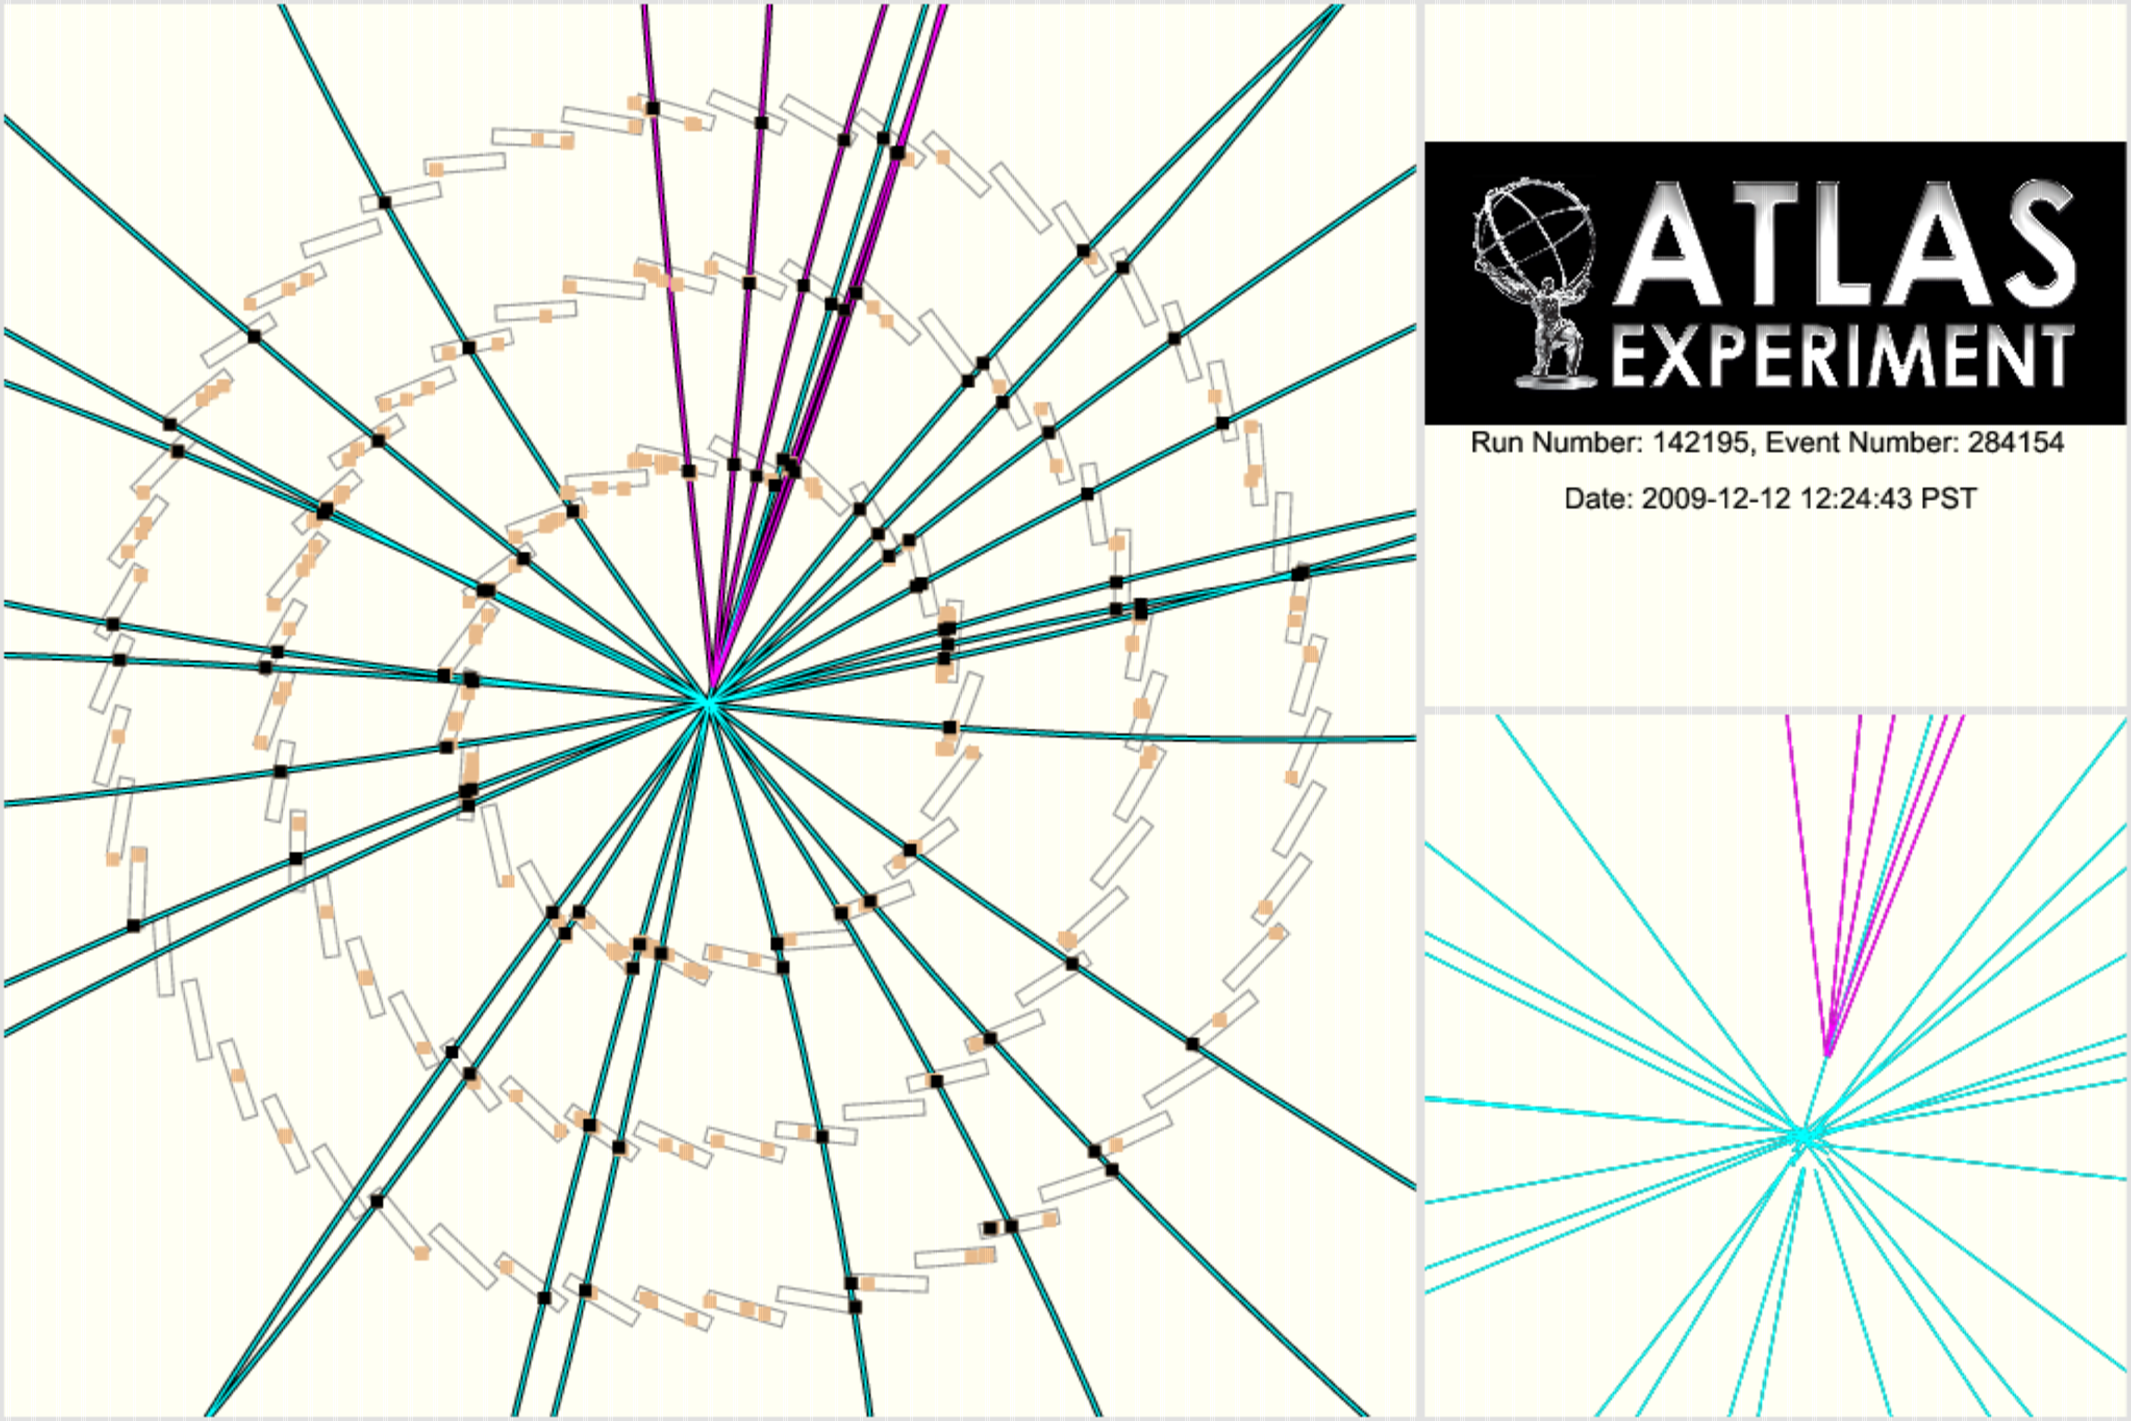
\includegraphics[width=0.8\textwidth]{ReconstructionPerformance/images/secondary_vertex.pdf}
	\caption{An event from early ATLAS data-taking, with a number of tracks (in teal) leading back to the primary vertex, and a secondary vertex reconstructed with the associated tracks highlighted in purple \cite{sv}.	\label{fig:secondary_vertex}  }
\end{figure}
%-----------------------------------------------------------------------------




There are several different $b$-tagging algorithms that exploit each of these features independently; however, if 
a jet truly comes from a $b$-quark, then several of these features can arise in the 
same jet and the correlation can be used to further increase the accuracy of the tagger.  That idea gives 
rise to the MV1 tagger (where the MV stands for ``multivariate''), a neural-net-based 
$b$-tagging algorithm that uses three other $b$-tagging algorithms (SV1, IP3D, JetFitter
) as inputs.   The performance curve for the MV1 algorithm can be seen in Figure~\ref{fig:mv1_roc}; 
for a typical $b$-jet efficiency of 70\% (meaning that 70\% of real $b$-jets 
are positively tagged by the algorithm), the light-jet rejection is about 99.5\% and the 
charm rejection is about 90\% \cite{b-tagging}.


%https://atlas.web.cern.ch/Atlas/GROUPS/PHYSICS/CONFNOTES/ATLAS-CONF-2014-046/fig_01.pdf
\begin{figure}
	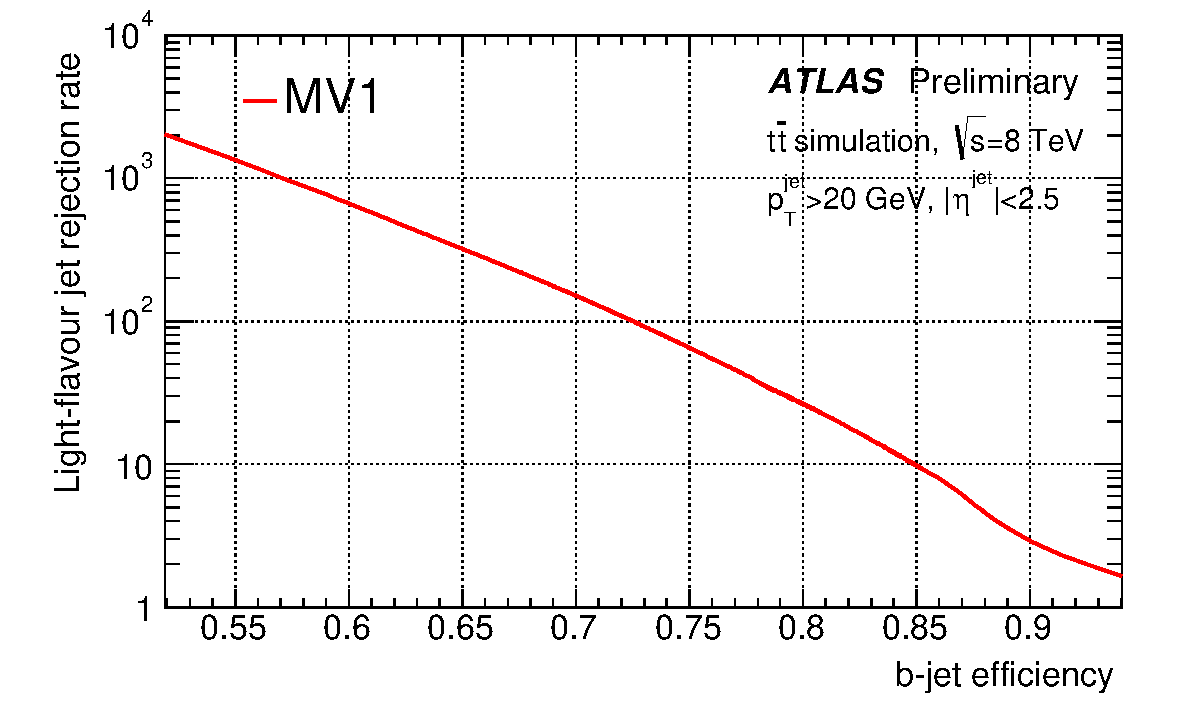
\includegraphics[width=0.8\textwidth]{ReconstructionPerformance/images/mv1_roc.pdf}
	\caption{secondary vertex \cite{b-tagging}	\label{fig:mv1_roc}  }
\end{figure}


















% Activate the following line by filling in the right side. If for example the name of the root file is Main.tex, write
% "...root = Main.tex" if the chapter file is in the same directory, and "...root = ../Main.tex" if the chapter is in a subdirectory.
 
%!TEX root =  

\chapter[MonteCarlo]{Monte Carlo}

In order to understand both the signal and backgrounds better, Monte Carlo (MC) datasets are computer-generated simulation events that allow a physicist to develop and validate an analysis.  The generation and refinement of MC algorithms and datasets could be a thesis in its own right, but this section will touch on some of the most relevant features of the MC datasets used in this algorithm.


\section{MC Creation Procedure}
\label{sec:mc-gen-overview}
MC events are generally created in four major steps.  
\begin{enumerate}
    \item First, the ``generator'' uses quantum field theory to simulate the hard scatter, generally starting with a proton and ending with all final-state particles.  
    \item Then those particles are handed off to a dedicated algorithm that simulates how they would shower and hadronize, where appropriate.  
    \item Next, the resulting particles from the first two steps are put into a detector simulation, which uses information on the detector materials and geometry to understand how the particles evolve as they travel through the ATLAS detector.  
    \item The detector's response to the particles is simulated in a digitization and reconstruction step, so that the final output is an event that looks similar to how a ``real'' event of that type might look in the ATLAS detector. 
\end{enumerate} 

\section{Signal Monte Carlo}
MadGraph \cite{MadGraph} is used to generate the signal MC, with showering and hadronization done in Pythia6 \cite{Pythia6}.  Madgraph uses a 5 flavor scheme PDF (parton distribution function), meaning that it models $b$-quarks in the proton as well as the more common light flavor (up, down, charm and strange quarks, and gluons).  In addition to the Higgs production with the associated $b$-quark and the Higgs decay, there can also be extra jets in the event from initial state radiation (ISR) and/or final state radiation (FSR).  We allow up to three additional partons per event in the signal MC; the generation and cross-section calculations tend to be more accurate for higher numbers of extra partons allowed but at the cost of exponentially slower and more complicated generation times.  We found three jets to be a reasonable cutoff where the distributions did not seem to be affected by allowing for higher numbers of extra partons, but the generation time was still acceptably quick.  

%--------------------------------------------------------
\begin{table}
   \caption{The signal MC samples and their parameters. \label{tab:sig_mc_parameters} }
    \begin{tabular}{ c c c }
    Dataset ID & mass (GeV) & width (GeV) \\
    181120     & 250        & 1.68682 \\
    181121     & 280        & 1.92318 \\
    181122     & 310        & 2.50849 \\
    181123     & 350        & 3.23507 \\
    181124     & 400        & 3.93561 \\
    181125     & 450        & 4.71906 \\
    181126     & 500        & 5.59454 \\
    181127     & 550        & 6.84368 \\
    181128     & 600        & 8.11044 \\
    181129     & 650        & 9.26688 \\
    181130     & 700        & 10.3760 \\
    181131     & 800        & 12.5049 \\
    \end{tabular}
\end{table}

%--------------------------------------------------------




The Madgraph signal generation is done for 12 different mass points, spanning 250-800 GeV. Below 250 GeV, the daughter $b$-jets from the Higgs tend to be too low-$p_T$ to fire the trigger, while above 800 GeV SUSY becomes less appealing theoretically.  Since both the production and decay of $bH\rightarrow bbb$ happen via SM interactions, with SUSY only becoming relevant for increasing the production cross section and widening the inherent width of the $A/H$ distributions, the signal generation can be done by using an SM $bH\rightarrow bbb$ production model but with a modified Higgs width.  There are 300,000 signal events generated for each mass point.

% ATF-II source: http://iopscience.iop.org/1742-6596/396/2/022031
The detector simulation for the signal MC was done using AtlFast-II (AFII) \cite{ATF2}, a modified version of Geant4 \cite{Geant4-1, Geant4-2} designed to cut down on the considerable time required for simulating particle interactions with the detector, especially showers in the calorimeter.  AFII does full simulation of the inner detector and tracking, but uses frozen shower shapes taken from a large collection of pre-generated samples to speed up the simulation.  After simulation, the digitization and reconstruction are handled by the ATLAS standard algorithms in the ATHENA framework, as is standard for all ATLAS MC.    

\section{Background}
\subsection{QCD Background}
Although QCD is the largest and most important background in this analysis, fully modeling it with QCD has some important drawbacks, which motivates our decision to use a mostly data-driven background estimation method.  That having been said, MC can still be a very valuable tool for making basic estimates and validating assumptions. 

There are two major types of QCD background in this analysis: first, when there is one or more mistakenly $b$-tagged light flavor or charm jets, which we call \textit{reducible} because, at least in theory, it could be identified and isolated/removed; and second, the \textit{irreducible} QCD background in which three real $b$-jets are present in the final state but without the intermediate resonance of the Higgs.  Both sources of background are expected to be significant but generally require different MC generation strategies.

\subsubsection{QCD Multijet}
The ATLAS QCD multijet MC collection is dataset is generated using Pythia8 \cite{Pythia8}.  One of the major challenges of a truly inclusive sample like this one is that low-$p_T$ jets dominate the production cross section but generally have very low efficiency through the triggers or analysis cut flows, which is addressed by generating events several times with filtering applied based on the $p_T$ of the leading jet.  This leads to a distinctive ``slice'' structure to the sample, where 8 different slices are generated, each with a different $p_T$ range for the leading jet, and then the slices are knitted together with different relative weights to produce an inclusive spectrum with high statistics at all $p_T$ values.  


ATLAS has a high-statistics inclusive QCD MC sample that is used primarily in this analysis for understanding the QCD background from mistagged charm and light flavor.  Since the sample is inclusive, there is no filtering on the flavor of the jets that are produced (although there is dedicated effort to have high-$p_T$ jets simulated with adequate statistics) and the vast majority of jets are light or charm jets.  As a result, while we use this sample to estimate the efficiency and flavor composition of the QCD production in ATLAS as a whole, a particularly important background (QCD $bbb$) is virtually absent from this sample.


\subsubsection{$b$-Enriched QCD Multijet}
\label{sec:bb_qcd_mc}
Since the inclusive QCD Multijet samples are inadequate for understanding the $bb$ and $bbb$ MC backgrounds, we generate a dedicated sample that undergoes filtering to enrich it in heavy flavor.  This sample is generated using Sherpa 1.4.3 \cite{Sherpa} and detector simulation is done with AFII.  This sample starts with a 5-flavor PDF that assumes massive $b$-quarks and 2, 3 or 4 final state partons; then a filter is applied that requires that the leading 2 partons in the event be true $b$-quarks as well as requiring that the leading parton have a $p_T$ of at least 55 GeV (the latter requirement helps keep an acceptable efficiency when the sample is passed through the trigger and offline cuts).
i

%---------------------------------------
\begin{table}[h]
 \begin{center}
    \begin{tabular}{l|r}
   subprocess      & cross section (pb)\cr \hline

$jj\rightarrow b\bar{b}jj$ & 58531 \cr
$jj\rightarrow b\bar{b}j$ & 33411 \cr
$bj\rightarrow bjj \ \ +\ \  \bar{b}j\rightarrow \bar{b}jj$ & 22147 \cr
$bj\rightarrow bjjj \ \ +\ \  \bar{b}j\rightarrow \bar{b}jjj$ & 16282 \cr
$bj\rightarrow b j \ \ +\ \  \bar{b} j\rightarrow \bar{b} j$ & 12135 \cr
$jj\rightarrow b\bar{b}$ &  1672 \cr
$cj\rightarrow c b\bar{b}j \ \ +\ \  \bar{c} j\rightarrow \bar{c}  b\bar{b}j$ & 1602 \cr
$bj\rightarrow b b\bar{b}j \ \ +\ \  \bar{b} j\rightarrow \bar{b}  b\bar{b}j$ & 997 \cr
$jj\rightarrow b\bar{b}c\bar{c}$ &  776 \cr
$cj\rightarrow c b\bar{b} \ \ +\ \  \bar{c} j\rightarrow \bar{c}  b\bar{b}$ & 681 \cr
$bj\rightarrow b b\bar{b} \ \ +\ \  \bar{b} j\rightarrow \bar{b}  b\bar{b}$ & 387 \cr
$jj\rightarrow b\bar{b}b\bar{b}$ &  376 \cr
$b\bar{c}\rightarrow b\bar{c}j \ \ +\ \  \bar{b} c\rightarrow \bar{b} cj$ & 206 \cr
$bc\rightarrow bcj\ \ +\ \  \bar{b}\bar{c}\rightarrow \bar{b} \bar{c}j$ & 194 \cr
$b\bar{c}\rightarrow b\bar{c}jj \ \ +\ \  \bar{b} c\rightarrow \bar{b} cjj$ & 143 \cr
$bc\rightarrow bcjj\ \ +\ \  \bar{b}\bar{c}\rightarrow \bar{b} \bar{c}jj$ & 136 \cr
$bc\rightarrow bc\ \ +\ \ \bar{b}\bar{c}\rightarrow \bar{b} \bar{c}$ & 122 \cr
$b\bar{c}\rightarrow b\bar{c} \ \ +\ \  \bar{b} c\rightarrow \bar{b} c$ & 121 \cr
$b\bar{b}\rightarrow b\bar{b}j$ & 62 \cr
$bb\rightarrow bbj\ \ +\ \  \bar{b}\bar{b}\rightarrow \bar{b} \bar{b}j$ & 53 \cr
$b\bar{b}\rightarrow b\bar{b}jj$ & 44 \cr
$bb\rightarrow bbjj\ \ +\ \  \bar{b}\bar{b}\rightarrow \bar{b} \bar{b}jj$ & 39 \cr
$b\bar{b}\rightarrow b\bar{b}$ & 37 \cr
$bb\rightarrow bb\ \ +\ \  \bar{b}\bar{b}\rightarrow \bar{b} \bar{b}$ & 30 \cr
\hline
   \end{tabular}
\caption{Hard subprocesses simulated in the bb QCD MC event sample, along with their cross sections. Here
$j=u,\bar{u},d,\bar{d},s,\bar{s},g$}
\label{tab:sherpa_subprocesses}
  \end{center}
\end{table}
%---------------------------------------



%-----------------------------------------------                     
\begin{figure}
  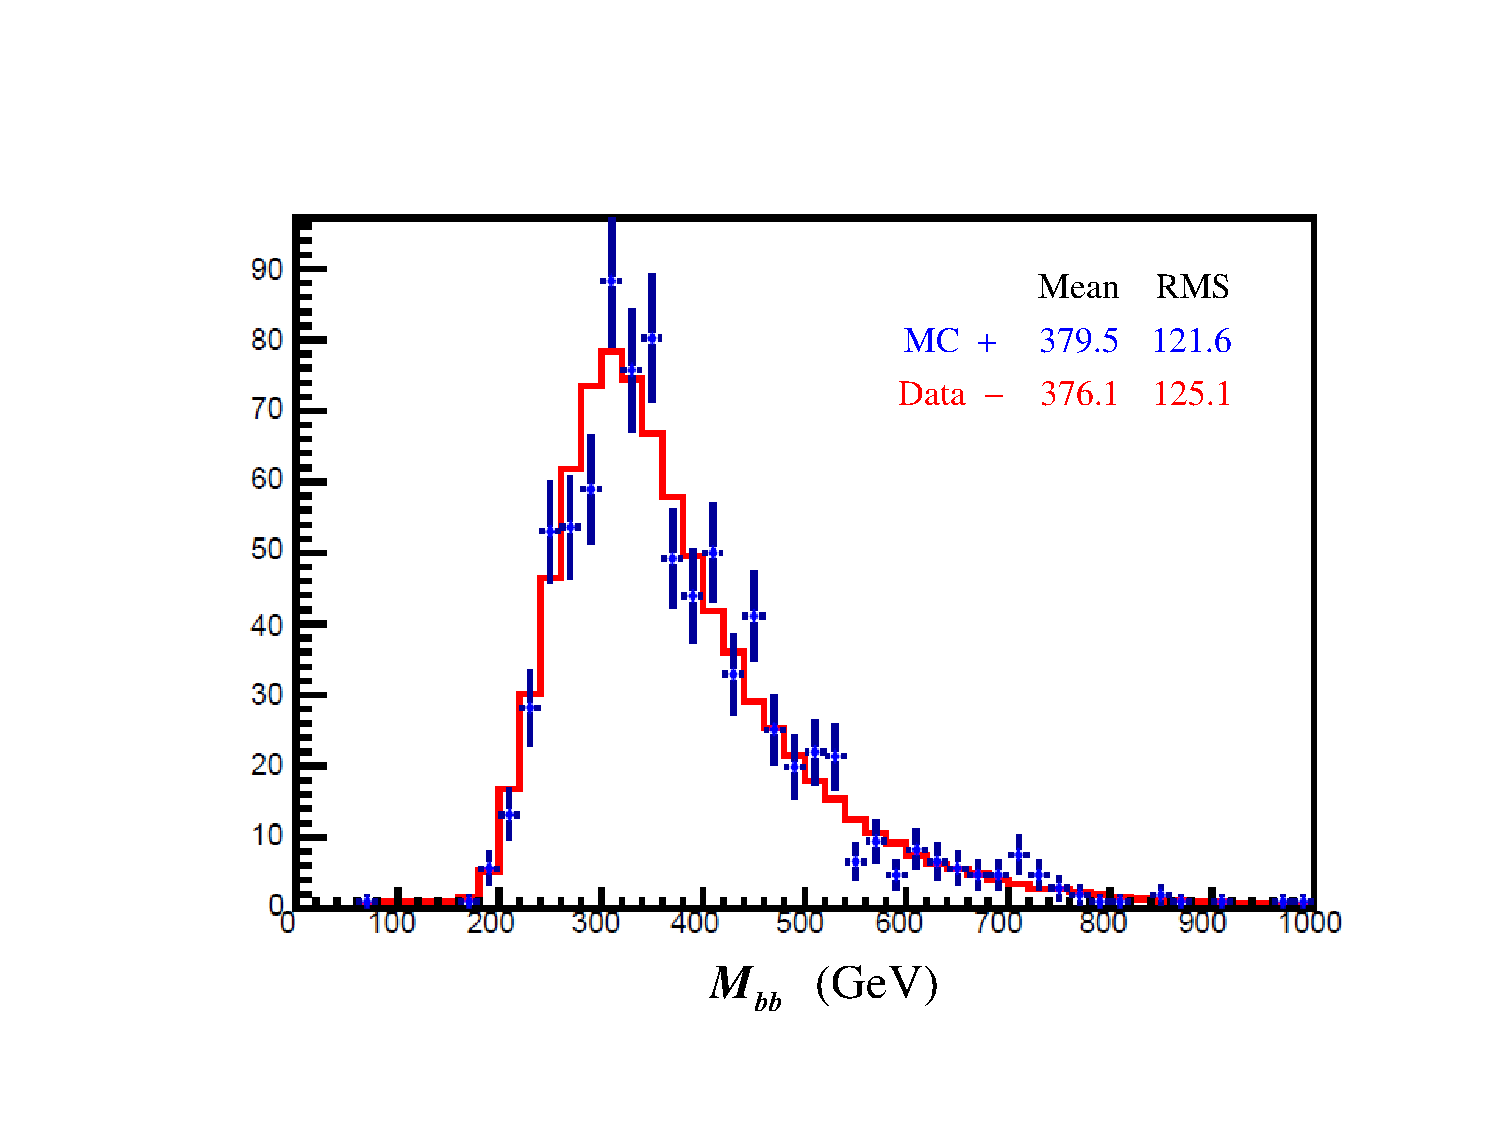
\includegraphics[width=0.70\linewidth]{MonteCarlo/figures/mbb_bbqcd_vs_data.pdf}
  \caption{Mass of the two leading jets in events passing all cuts except the
bbb, bbloose and bbanti classification.  Distributions for the 10,000 event bb QCD Monte Carlo validation sample
and a 2.2~fb$^{-1}$ luminosity data sample are shown.    \label{fig:mbb_bbqcd_vs_data}}
\end{figure}

\begin{figure}
  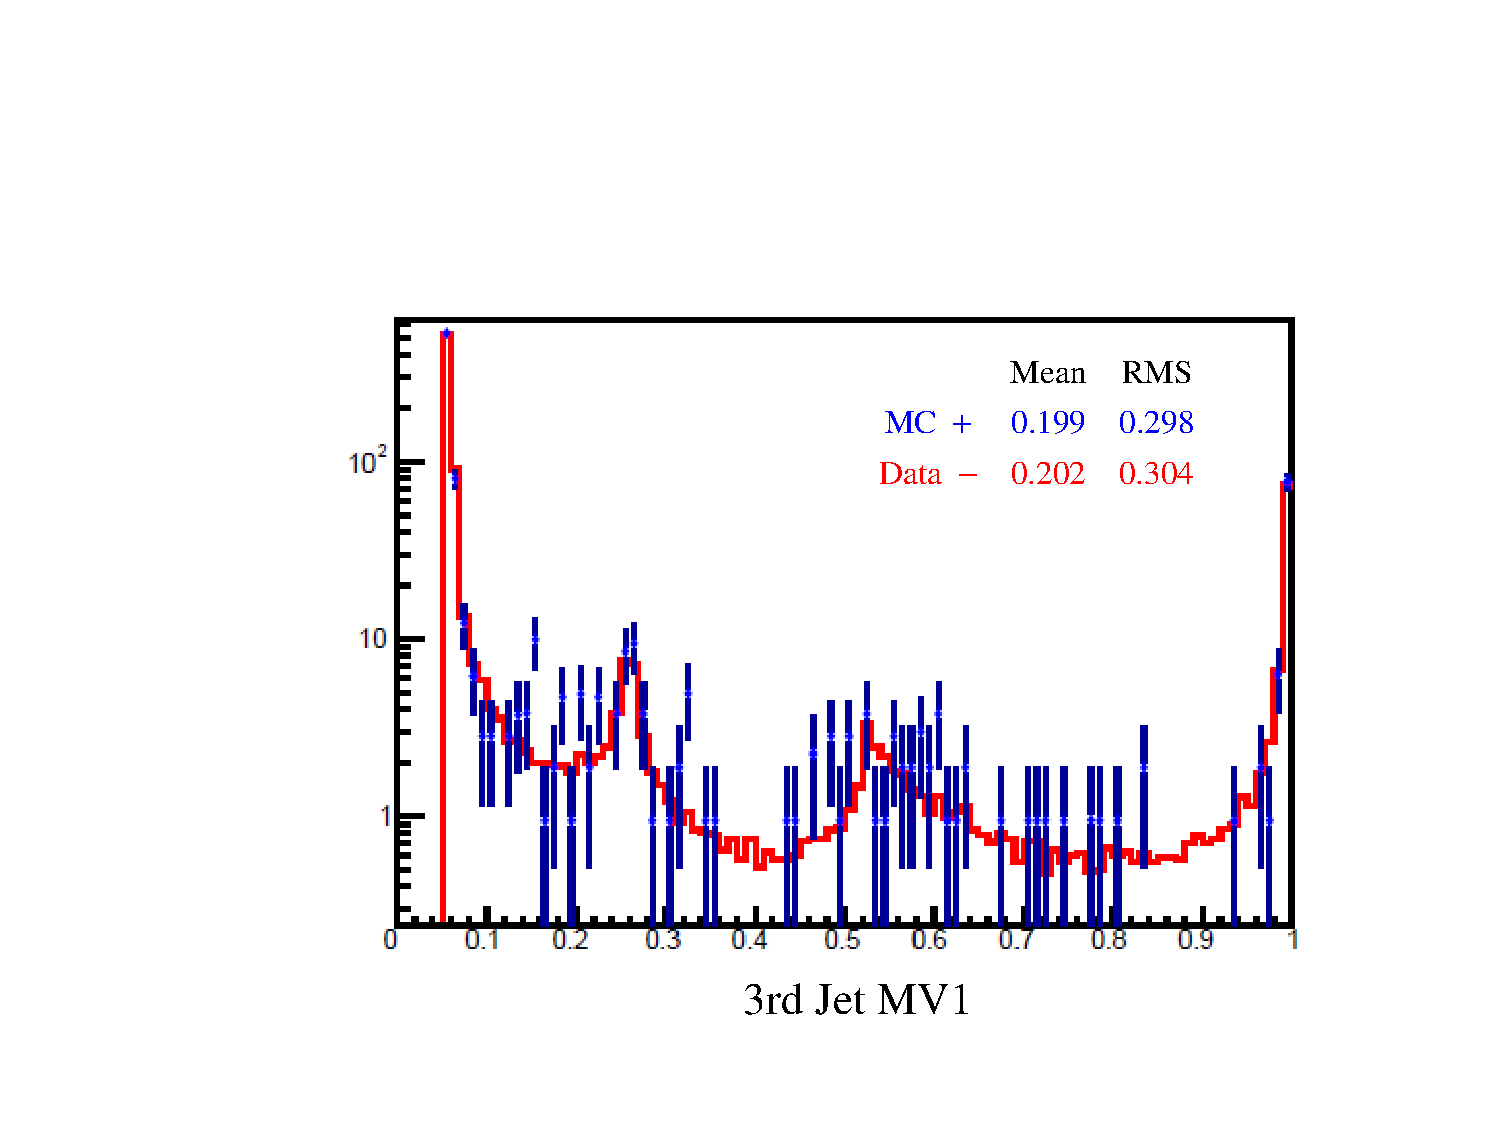
\includegraphics[width=0.70\linewidth]{MonteCarlo/figures/mv1_jet3_bbqcd_vs_data.pdf}
  \caption{The b-tag variable MV1 for the 3rd leading $p_T$ jet in events passing all cuts except the
bbb, bbloose and bbanti classification.     Distributions for the 10,000 event bb QCD Monte Carlo validation sample
and a 2.2~fb$^{-1}$ luminosity data sample are shown.    \label{fig:mv1_jet3_bbqcd_vs_data}}
\end{figure}




\begin{figure}
  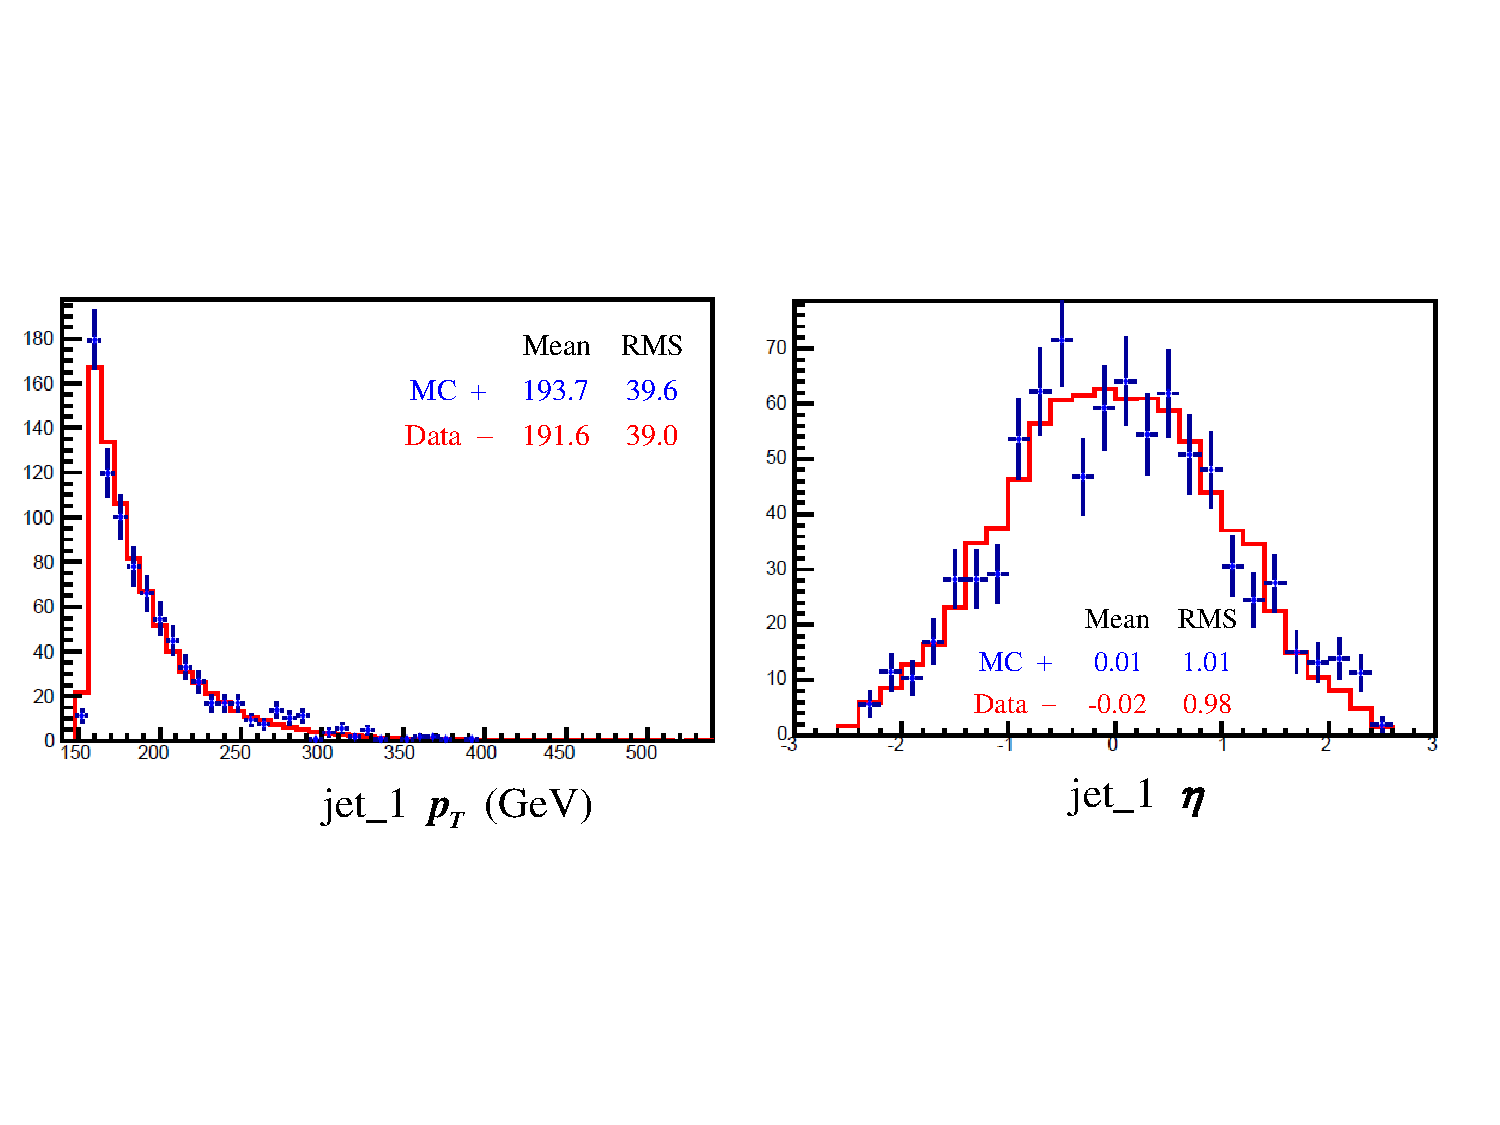
\includegraphics[width=0.85\linewidth]{MonteCarlo/figures/pt_eta_jet1_bbqcd_vs_data.pdf}
  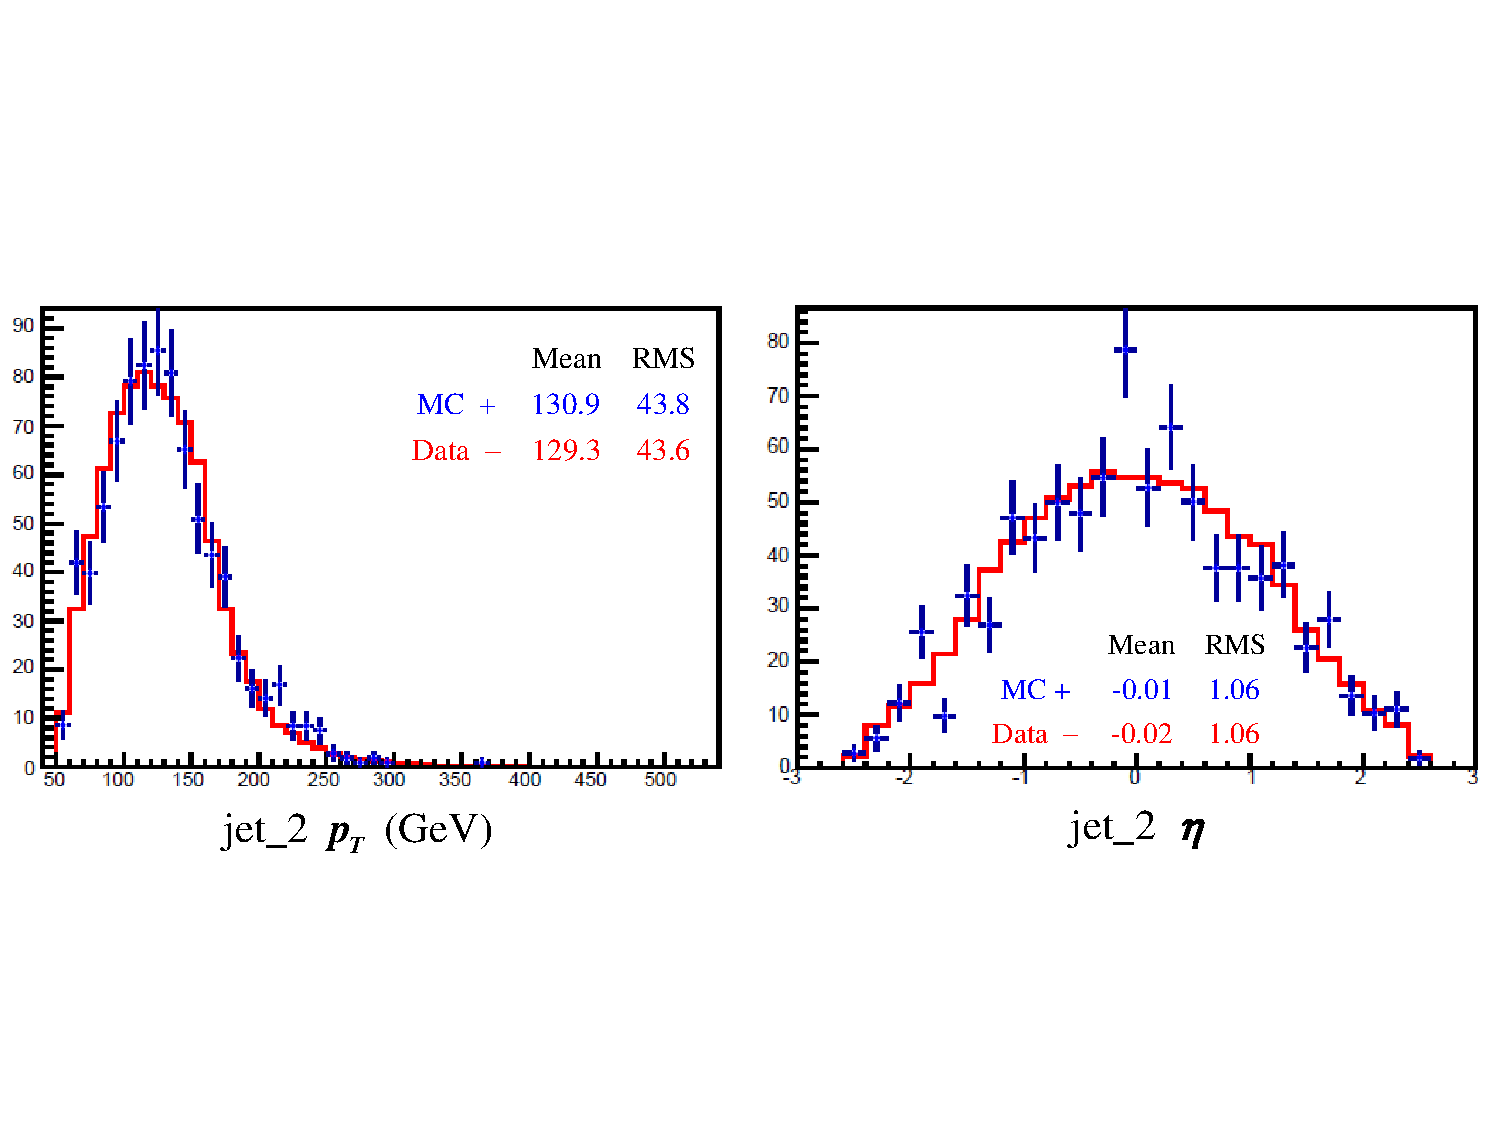
\includegraphics[width=0.85\linewidth]{MonteCarlo/figures/pt_eta_jet2_bbqcd_vs_data.pdf}
  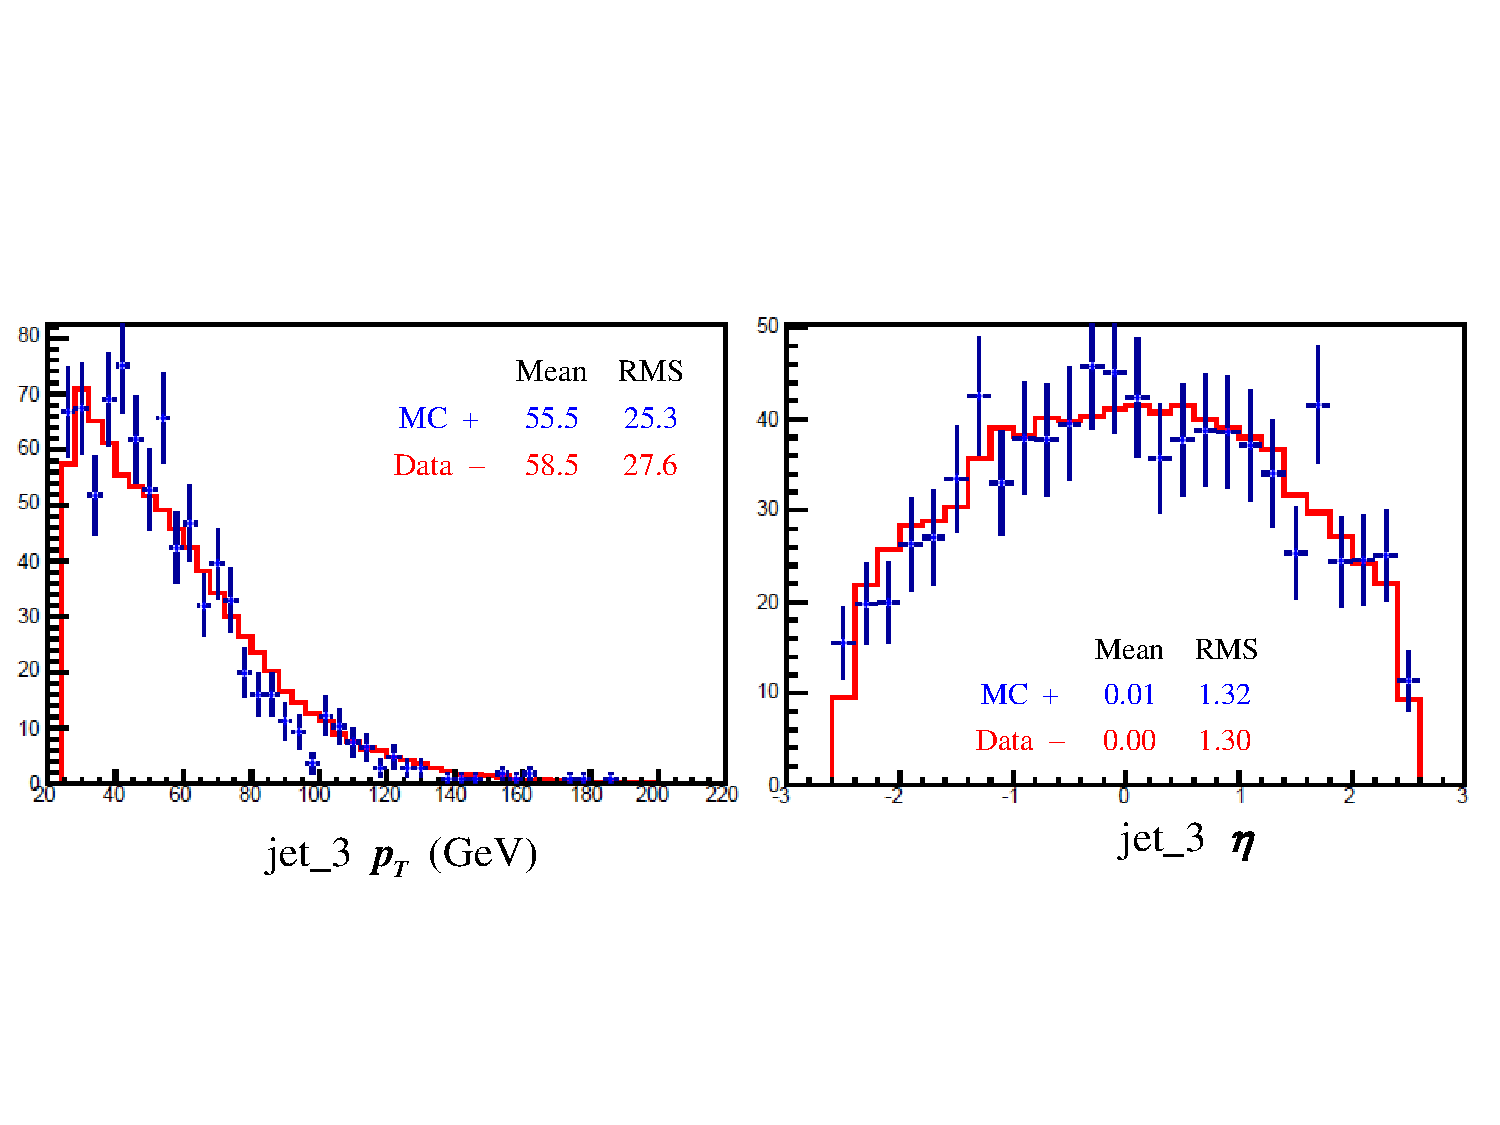
\includegraphics[width=0.85\linewidth]{MonteCarlo/figures/pt_eta_jet3_bbqcd_vs_data.pdf}
  \caption{$p_T$ and $\eta$ for the three leading $p_T$ jets in events passing all cuts except the
bbb, bbloose and bbanti classification.     Distributions for the 10,000 event bb QCD Monte Carlo validation sample                 
and a 2.2~fb$^{-1}$ luminosity data sample are shown.    \label{fig:pt_eta_bbqcd_vs_data}}                                          
\end{figure}                                                                                                                        
%-----------------------------------------------                     



\subsection{Top Background}
Top-antitop pairs decaying all-hadronically is the largest non-QCD background.  The sample generated
to model this background is generated in Powheg and Pythia, with Tauola and Photos also used for
handling tau leptons and photons.  In practice, $t\bar{t}$ is a minor background, both because
of its small cross section relative to QCD and because in the high mass ranges most relevant for
this search, it does not show any sigificant structure or $m_{bb}$ shape differences depending
on the flavor of the third jet.


\begin{table}
   \caption{Parameters of the $t\bar{t}$ MC sample used in this analysis. \label{tab:ttbar_params} }
    \begin{tabular}{ c c c c }
    Dataset ID & Cross Section [nb] & Filter Efficiency & N Events \\
    117050     & 0.21085        & 0.54298    & 99930891 \\
    \end{tabular}
\end{table}

%--------------------------------------------------------








% Activate the following line by filling in the right side. If for example the name of the root file is Main.tex, write
% "...root = Main.tex" if the chapter file is in the same directory, and "...root = ../Main.tex" if the chapter is in a subdirectory.
 
%!TEX root =  ../Thesis.tex

\chapter[Trigger and Cuts]{Trigger and Cuts}

The very first steps of any analysis consist of gathering the data, and then reducing the background
as much as possible.  For an experiment like ATLAS, with a dataset that approaches 3 PB of raw
data collected per year, picking a subset of that data for performing the search is both nontrivial
and crucial to the overall success of an analysis.  

The data selection starts with the trigger, which determines which events will even be recorded in the
first place.  The trigger must balance the competing forces of signal processes that can be very rare
(which would suggest a permissive trigger, so as to not lose already-rare signal events) and the
huge background rates at the LHC (which would suggest a strict trigger).  Since the trigger must make
decisions about event acceptance in near real-time, it can generally only require basic physics objects
like jets and $b$-tags, and more sophisticated background rejection gets implemented as offline event 
selection criteria, also called cuts.  

 
\section{Trigger}
\label{sec:my_trigger}
The purpose and structure of the ATLAS trigger are explained in Section~\ref{sec:atlas_trig}.
  The trigger chain for this analysis is as follows: 

\begin{itemize}
    \item L1: At least one J75 RoI\footnote{RoI stands for region of interest, an ATLAS acronym
    for a physical area in the calorimeter which has a large number of adjacent firing calorimeter
    cells, which collectively serve as a jumping-off point for a jet clustering algorithm}, implying an L1 jet of at least 75 GeV
    \item L2: least two 30 GeV jets, of which one must be at least 140 GeV. Additionally, at least two
jets must satisfy a medium b-tag (L2 xComb\footnote{xComb is the name of the $b$-tagging algorithm
that is used in the trigger; L2 refers to the version of xComb being run at L2 of the trigger} $>$ 1.276)
    \item EF: At least two 35 GeV jets, of which one must be at least 145 GeV. Additionally, at least two
jets must satisfy a medium $b$-tag (EF xComb\footnote{xComb is used in both L2 and EF of the trigger;
the values of the inputs to the algorithm can change between L2 and EF as more computationally intensive
reconstruction techniques are used in EF compared to L2} $>$ 1.099). There is no explicit requirement that the
b-tagged jets from L2 correspond with the $b$-tagged jets from EF. However, as detailed later, this
requirement is added later as an offline cut.
\end{itemize}


In the trigger, the L2 and EF jets are b-tagged using xComb, a likelihood ratio of IP3D\footnote{IP3D, like
the other algorithms described here, uses statistical learning algorithms trained on a large sample
of Monte Carlo simulation events to predict whether a given jet is a $b$-jet or not.  The various $b$-taggers
vary in the algorithm and input features, which are very briefly summarized in this list. } 
(significance of $z_0$ and $d_0$ impact parameters), SV1 (mass of the secondary vertex), NVTX (the number of
vertices with two tracks), and EVTX (the energy fraction of the secondary vertex), as well as the number
of vertices with 2 tracks. The triggers in this analysis use the medium operating point, such that L2 xComb
$>$ 1.276 and EF xComb $>$ 1.099.  This is the loose working point, where the $b$-jet efficiency
is 70\% online.

Table~\ref{tab:online_offline_btag} below shows the correlations between the two levels of online
$b$-tagging, as well as the offline (MV1) $b$-tagging for three offline working points (60\%, 70\%,
80\%).  

  \begin{table}[hbt]
\caption{  The acceptance of a cut on variable X given that the events have
  already passed (sig-like) or failed (bkgd-like) a cut on variable Y.\label{tab:online_offline_btag}}
    
    \begin{center}
    \begin{tabular}{l | l | c | c || c | c } \hline \hline
    \multicolumn{2}{c}{}  & \multicolumn{2}{c}{Signal MC} & \multicolumn{2}{c}{Unbiased Data} \\ \hline
      X         & Y         & sig-like & bkgd-like   &   sig-like & bkgd-like \\
      \hline
      EF        & L2        & 0.917    & 0.248 &   0.424       & 0.035 \\
      \hline
      L2        & MV1 (80)  & 0.675    & 0.031 &       0.510       & 0.077 \\
      EF        & MV1 (80)  & 0.824    & 0.090 & 0.515       & 0.050\\
      L2 and EF & MV1 (80)  & 0.676    & 0.036 & 0.414       & 0.031 \\
      MV1 (80)  & L2 and EF & 0.977    & 0.434 & 0.640       & 0.076 \\
      \hline
      L2        & MV1 (70)  & 0.716    & 0.060 & 0.652       & 0.086\\
      EF        & MV1 (70)  & 0.867    & 0.131 & 0.665       & 0.060 \\
      L2 and EF & MV1 (70)  & 0.721    & 0.060 & 0.563       & 0.038\\
      MV1 (70)  & L2 and EF & 0.954    & 0.340 & 0.538       & 0.034\\
      \hline
      L2        & MV1 (60)  & 0.757    & 0.101 & 0.762       & 0.095\\
      EF        & MV1 (60)  & 0.903    & 0.193 & 0.779       & 0.070 \\
      L2 and EF & MV1 (60)  & 0.765    & 0.103 & 0.692       & 0.045\\
      MV1 (60)  & L2 and EF & 0.902    & 0.250 & 0.429       & 0.015\\ \hline
    \end{tabular}
    \\
    \vspace{2mm}
    \end{center}
  \end{table}
  


%------------------------------------------------------
\begin{figure}
    \center
	\begin{subfigure}[L2 and EF $b$-tags]{0.45\textwidth}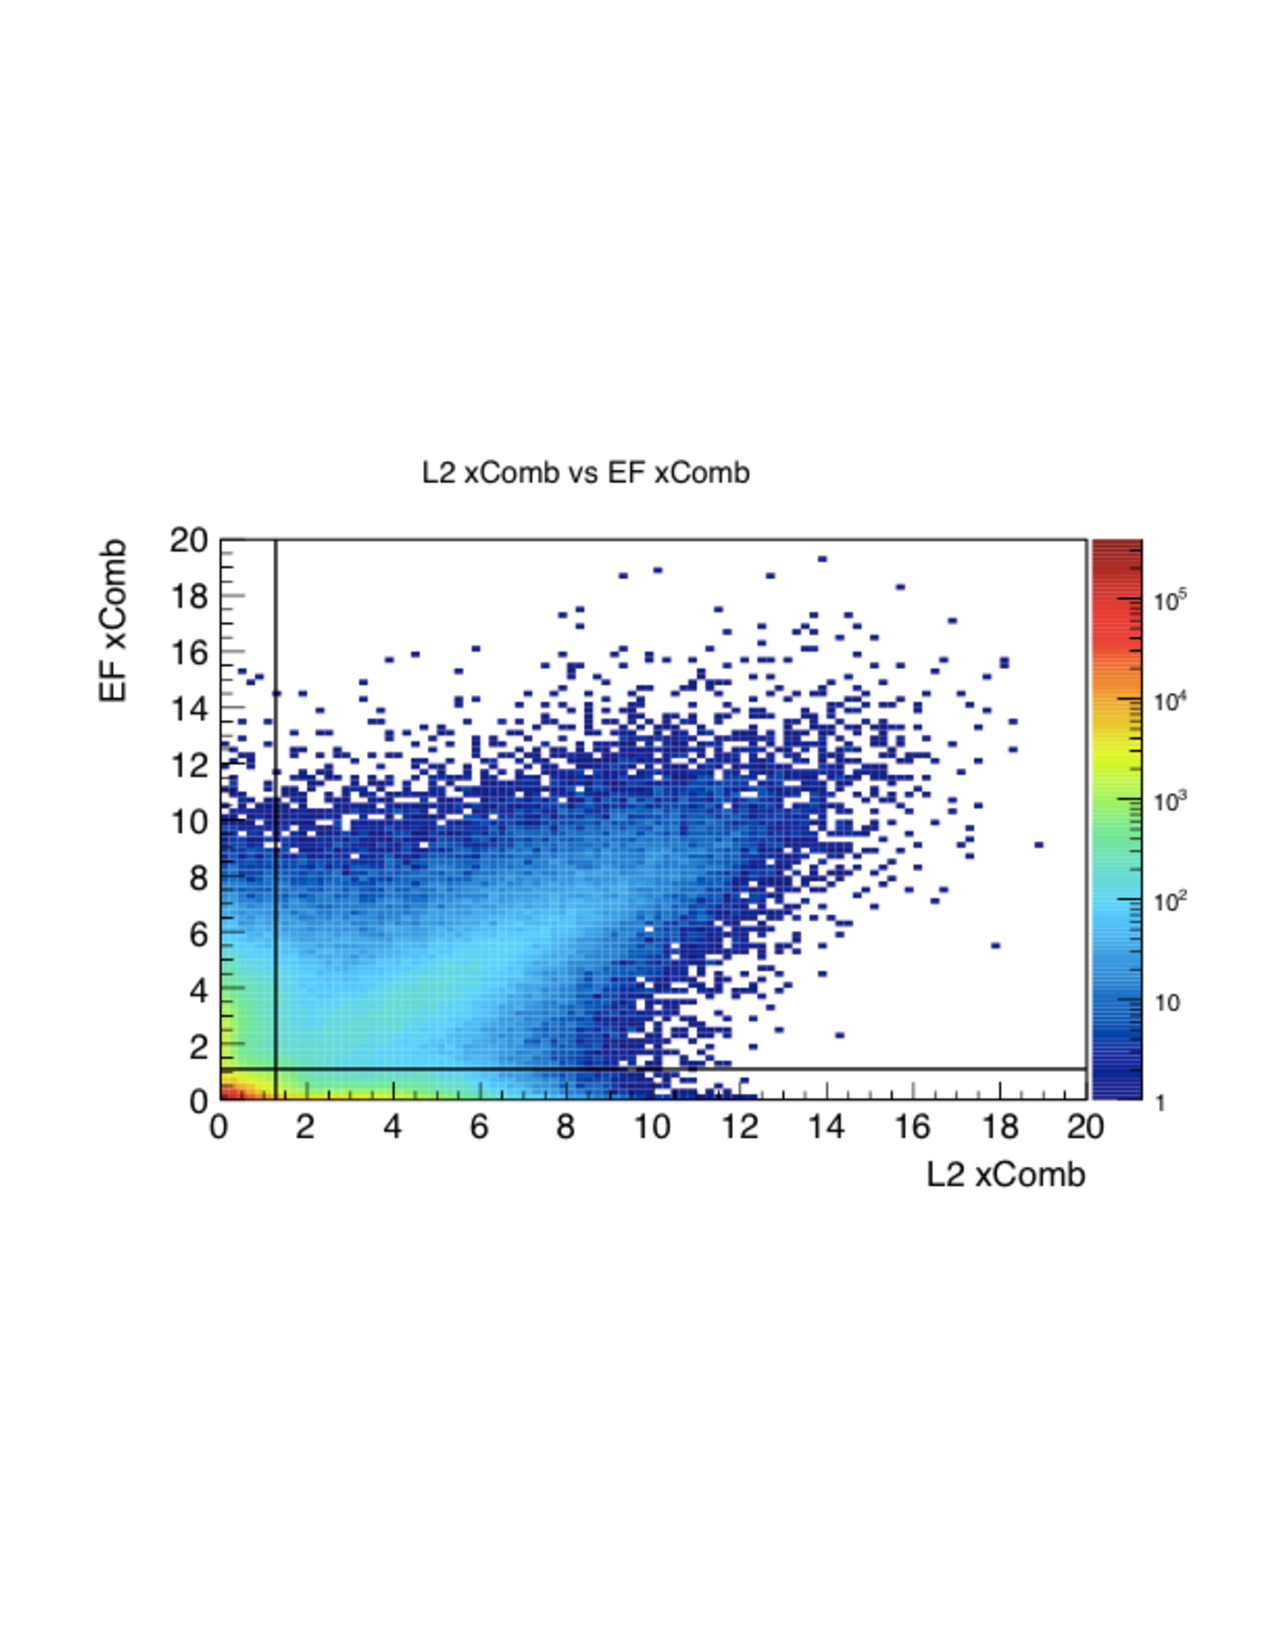
\includegraphics[width=\textwidth]{TriggerCuts/L2_EF.pdf}\end{subfigure}
	\begin{subfigure}[EF and MV1 $b$-tags]{0.45\textwidth}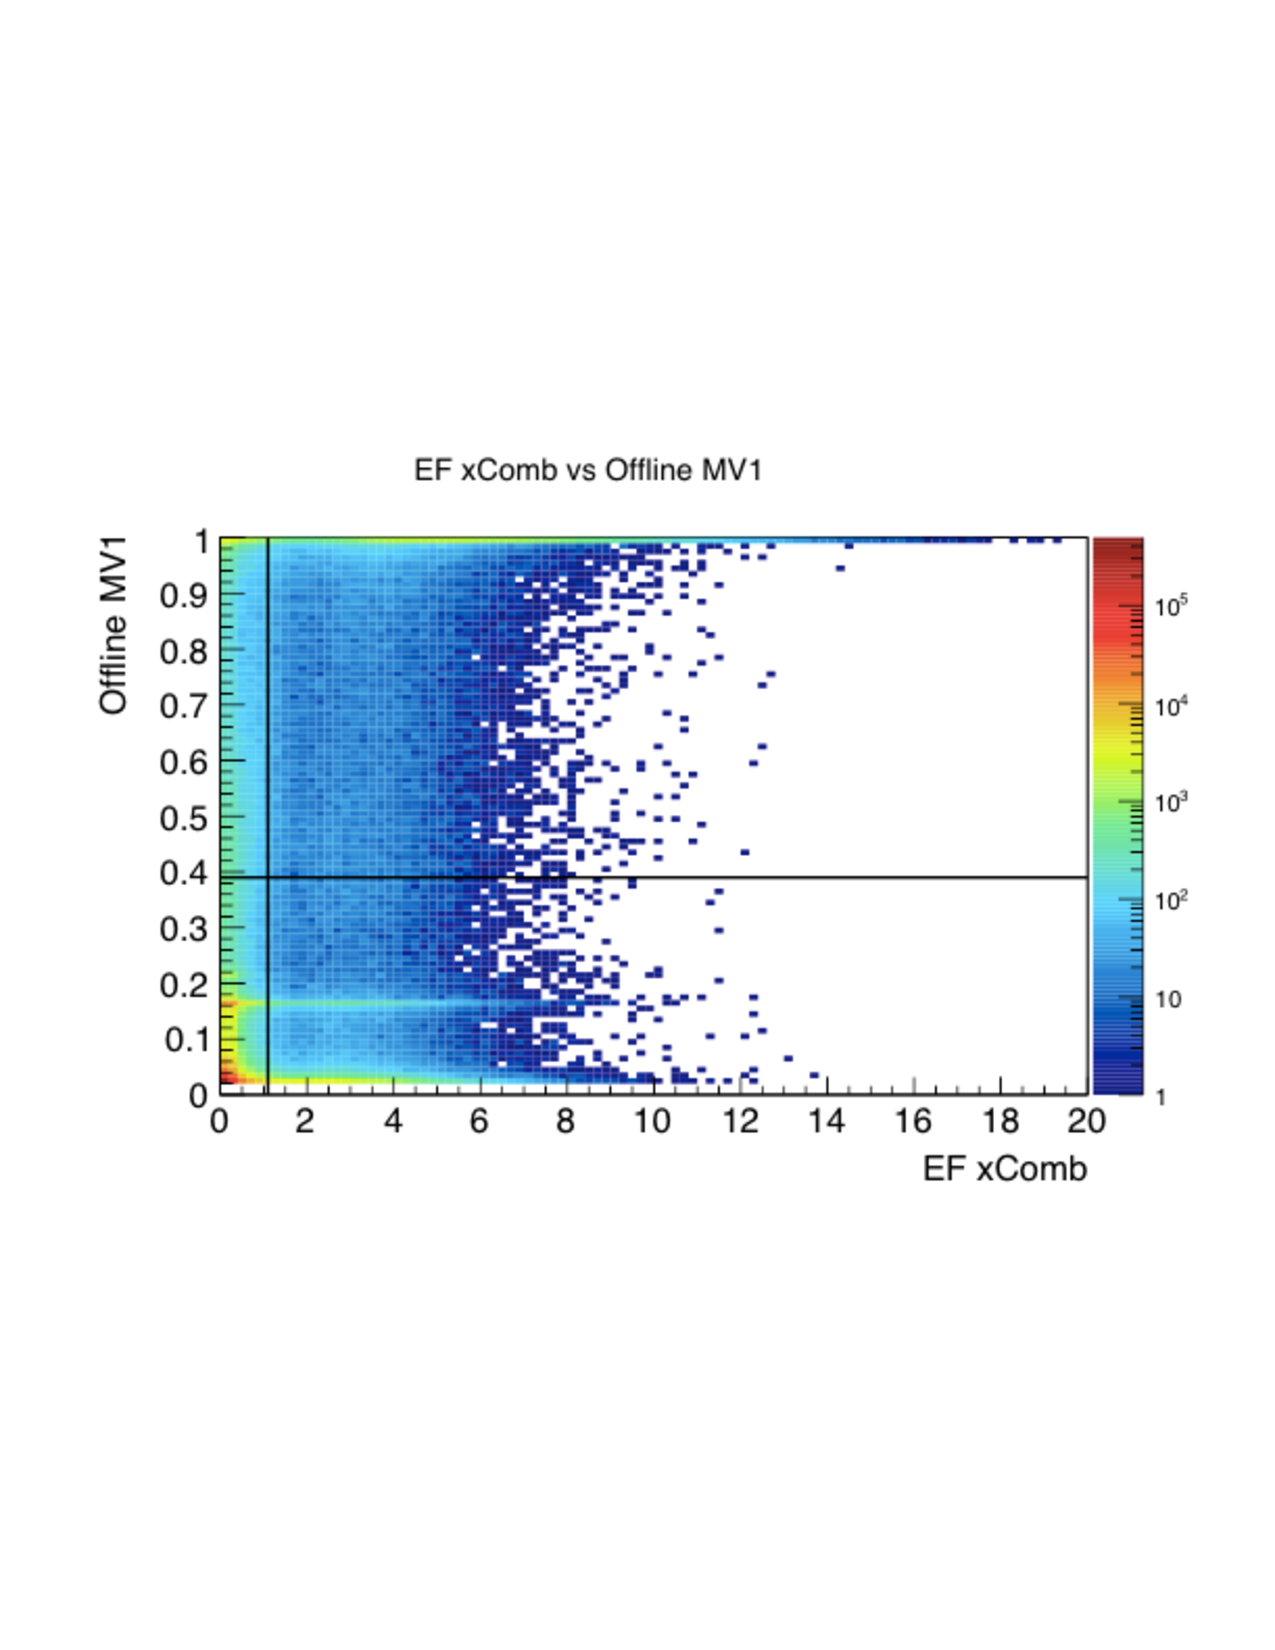
\includegraphics[width=\textwidth]{TriggerCuts/EF_MV1.pdf}\end{subfigure}
%  \begin{subfigure}[$m_{A}=550$ GeV]{0.4\textwidth}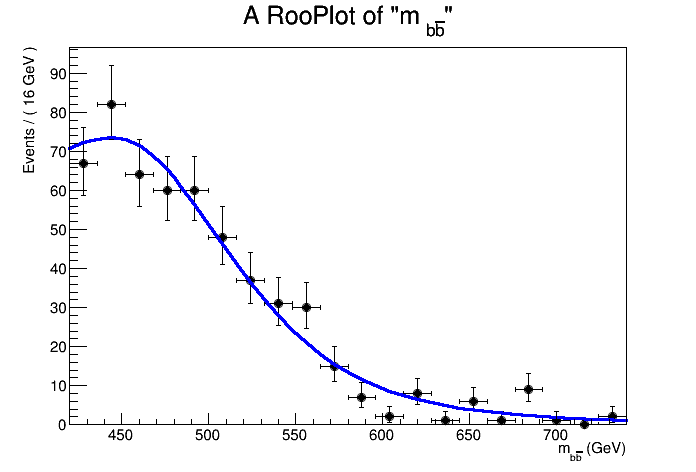
\includegraphics[width=\textwidth]{FitResults/images/fitMC_bAbb550_6.png}\end{subfigure}
    \caption{The $b$-tagging in Level 2 and 
    the Event Filter (in the trigger) and the MV1 $b$-tagging algorithm
    (offline) are exploited in the cut flow by requiring that at least
    2 jets in the event be ``triple tagged'', or $b$-tagged in both
    stages of the triggers as well as offline.  The figure on the
    left shows the L2 and EF $b$-tag distributions, on the right are the
    EF and MV1 distributions.  The cut points are noted with vertical
    and horizontal lines.  Most of the events (more than 80\%) fall
    in regions where the $b$-tagging cuts agree on whether a jet is 
    a $b$-jet or not, but a significant subsample of jets are tagged by 
    on $b$-tagging level/algorithm but not the other(s). \label{fig:L2_EF}}
\end{figure}

%------------------------------------------------------










\section{Offline Baseline Cuts}


\begin{itemize}
\item
\textbf{$p_T$ cuts of 155 and 55 GeV on leading and sub-leading jets, respectively.}
In order to get out of the \pt turn-on curves of the trigger, cuts of
155~GeV and 55~GeV are applied to the leading and second jets in the
event.
\item
\textbf{$p_T$ cut of 25 GeV on third jet.}
A third jet is not required by the trigger, but is required by
the offline cuts, and it must have a \pt greater than 25 GeV.  There is
no veto on additional jets.  Further details on the jet cuts can be found
in Section~\ref{sec:jet_reco}.
\item
\textbf{Two jets passing online (L2 and EF in trigger) and offline (MV1) $b$-tags}
As part of the trigger, two jets are required to be $b$-tagged at L2 and at EF.  It
is not explicitly required by the trigger that the same jets pass $b$-tagging at the two trigger levels,
or that those jets be tagged offline by the MV1 algorithm, so we make an
offline cut that imposes that requirement.  There is further discussion of the online
and offline $b$-tagging correlations in Section~\ref{sec:online_btagging},
where one of the important conclusions is that there is not perfect correspondence
between jets passing the three levels of $b$-tagging (L2, EF, MV1).  For
example, a jet with a large xComb value at L2 (and passing the $b$-tagging
requirement at L2) might have a small xComb value at EF (and fail the $b$-tagging
requirement at EF).  Likewise with L2 and MV1, or EF and MV1.  As a result, we
make an explicit requirement offline that the same two jets be $b$-tagged in L2, EF
and MV1.  Jets that are tagged in both L2 and EF of the trigger are referred to as
``trigger-tagged'' jets, and jets that pass L2, EF and MV1 are called ``triple-tagged''
jets.
The offline cut on the
trigger-matched $b$-jets is set to the 60\% efficiency
operating point. Due to the bias introduced by the trigger (see
Table~\ref{tab:online_offline_btag}), this provides additional rejection of
light jets for a relatively small decrease in signal efficiency.


\item\textbf{Leading 2 jets must pass tight MV1 $b$-tag}
It is also required that the two jets in the event with the highest \pt be $b$-tagged
offline by the MV1 algorithm.  There is no explicit requirement that the leading
two jets be trigger-tagged or triple-tagged.
  In addition to preferentially keeping signal events at a higher rate than
background events, this cut considerably improves the combinatorics of reconstructing
the Higgs and we see markedly better signal mass peak resolution when this cut is in
place.  Further details can be found in Section~\ref{sec:combinatorics}.


\item
\textbf{Categorization based on $b$-tagging of a 3rd jet}
After two
$b$-jets have been triple-tagged, the event is categorized based on whether
a third $b$-tagged jet is present.  The most signal-enriched region is where
a third jet passes a tight (60\% efficiency) MV1 $b$-tag; the next most
signal-enriched region is when no jets in the event pass a 60\% $b$-tag
but there is at least one jet passing a loose (80\% efficiency) $b$-tag;
the least sensitive region has no additional jets passing either 60\% or 
80\% $b$-tags (besides the triple-tagged jets).  These tag categories are
mutually exclusive and all have different signal enrichments, kinematics, 
and provide varying levels of sensitivity when used in the fit (Section~\ref{sec:background_strategy}).

\item
\textbf{Categorization based on the number of jets in the event}
Similarly, the events are categorized into 3-jet, 4-jet, and 5 (or more) jet
categories, primarily because the varying signal resolution in the different
jet bins leads to different signal to background ratios, and separating
the categories allows for extra sensitivity to be extracted (Section~\ref{sec:n_jets_sig}).
%The light-jet efficiency for this working point is approximately 0.1\%, and the
%charm efficiency is approximately 10\%.

\item 
\textbf{Rotation into Eigenbasis, and $p_T^{'}$ cuts}
After all the preceding precuts and categorizations are applied, the events
are rotated into a new basis based on the eigenvectors of the matrix composed of the
signal $m_{bb}$ and the $p_T$s of the leading 2 jets in the event.  Then cuts
based on the new (rotated) $p_T$s of the jets are applied, and the rotated $m_{bb}$
is used as the final discriminating variable.  Much more detail about this procedure,
its motivation and results, can be found in Section~\ref{sec:rotation}).



\end{itemize}



%------------------------------------------------------
\begin{figure}
    \center
	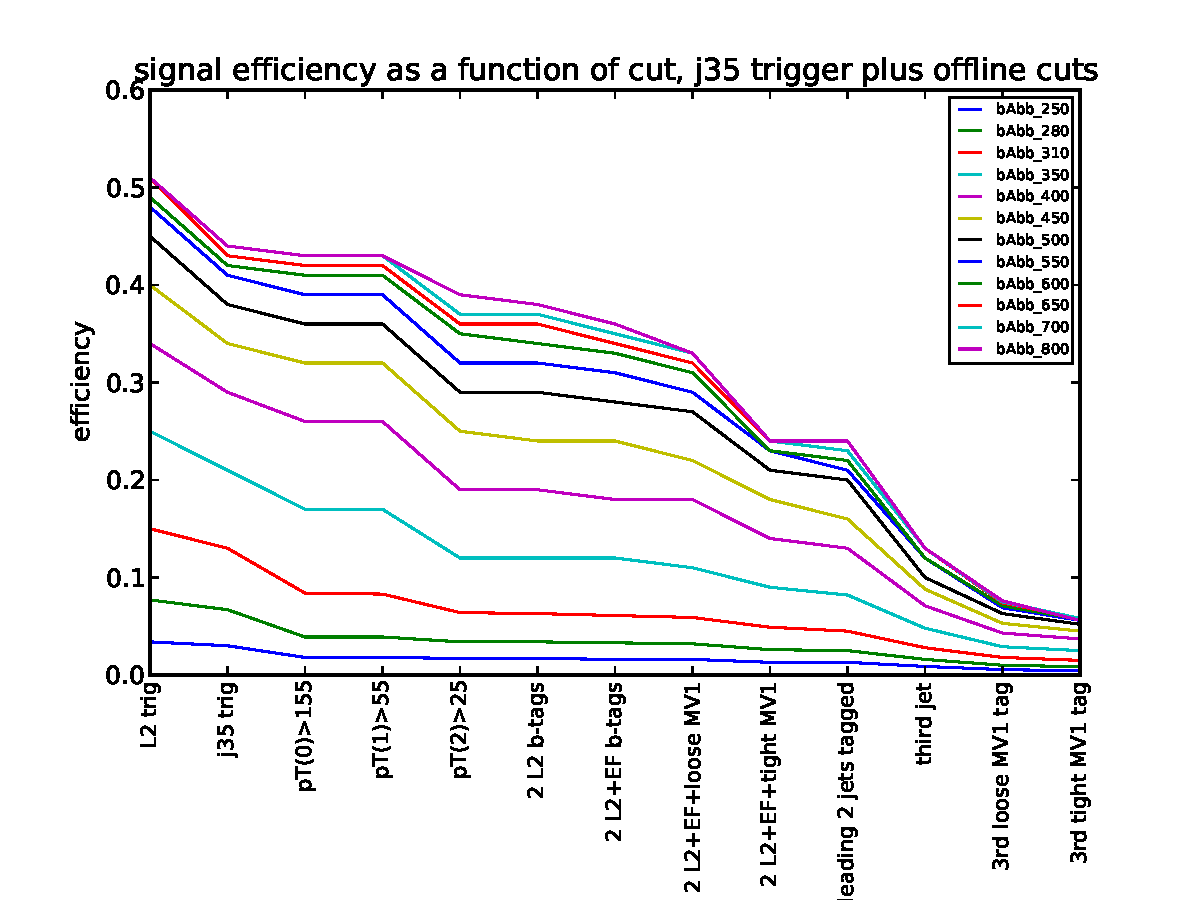
\includegraphics[width=0.98\textwidth]{TriggerCuts/cut_efficiencies_j35_signal.pdf}	
%	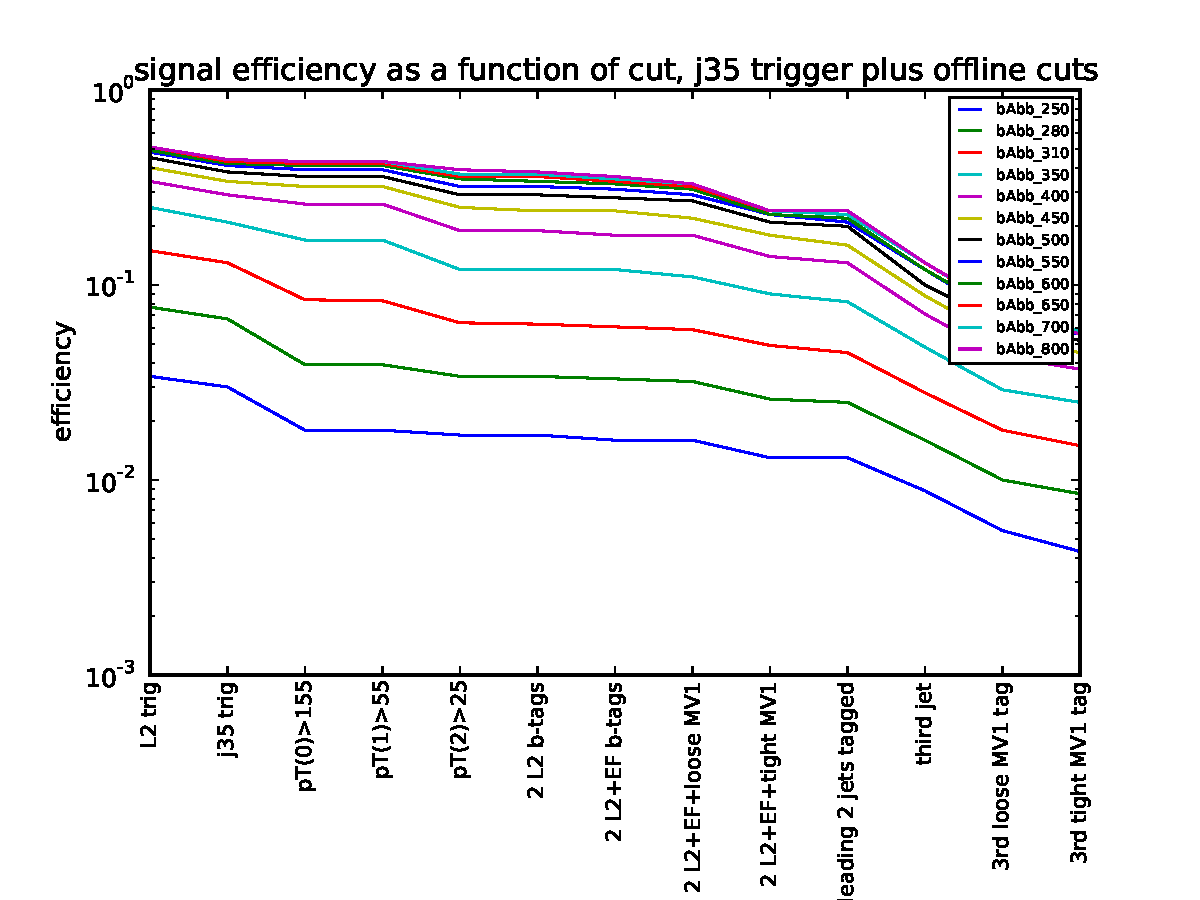
\includegraphics[width=0.98\textwidth]{TriggerCuts/cut_efficiencies_logy_j35_signal.pdf}	
    \caption{The cut efficiencies in signal, cut by cut.  Each line is a different
    signal mass point, and the overall trend is for higher efficiencies for the higher-mass
    particles than for the lower-mass particles. \label{fig:signal_eff_cutflow}}
\end{figure}

%------------------------------------------------------





%------------------------------------------------------
\begin{figure}
    \center
	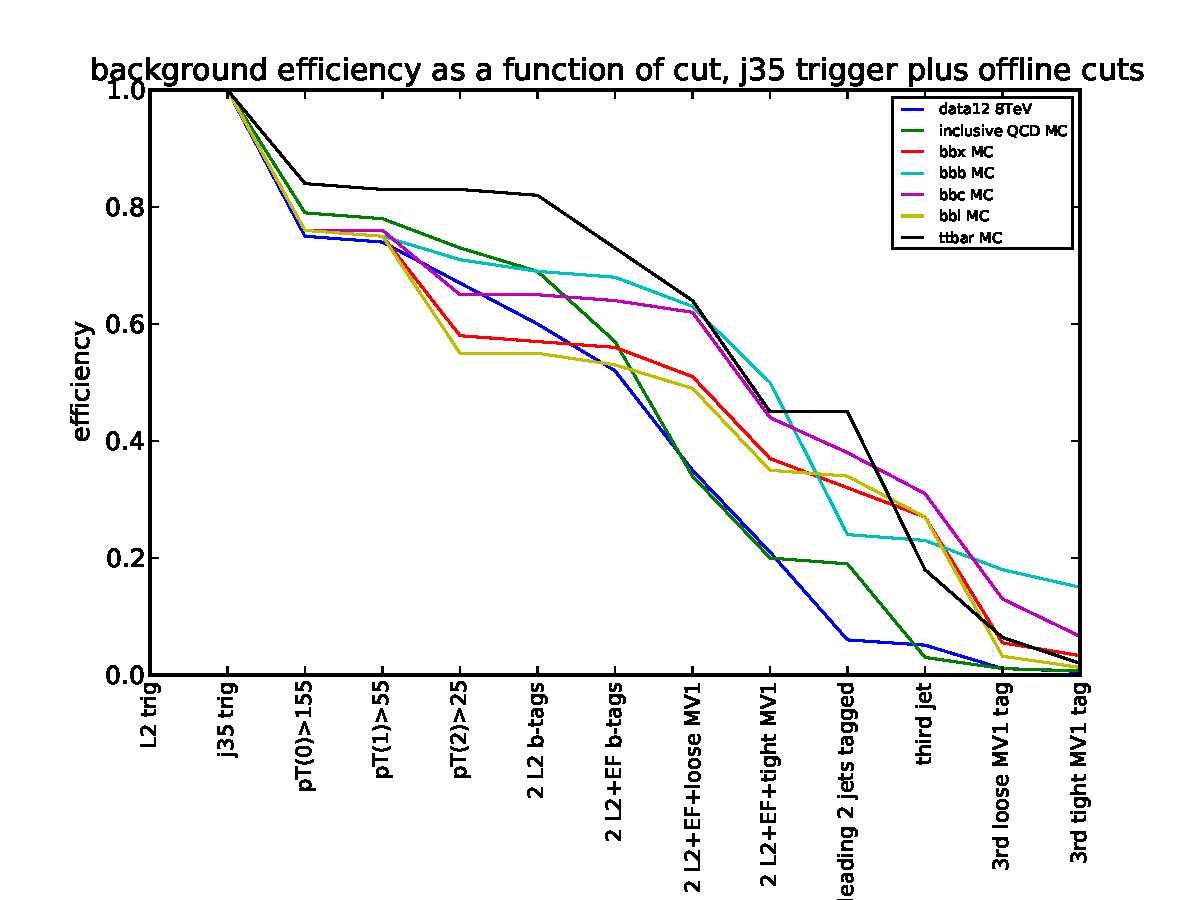
\includegraphics[width=0.98\textwidth]{TriggerCuts/cut_efficiencies_j35_background.pdf}	
%	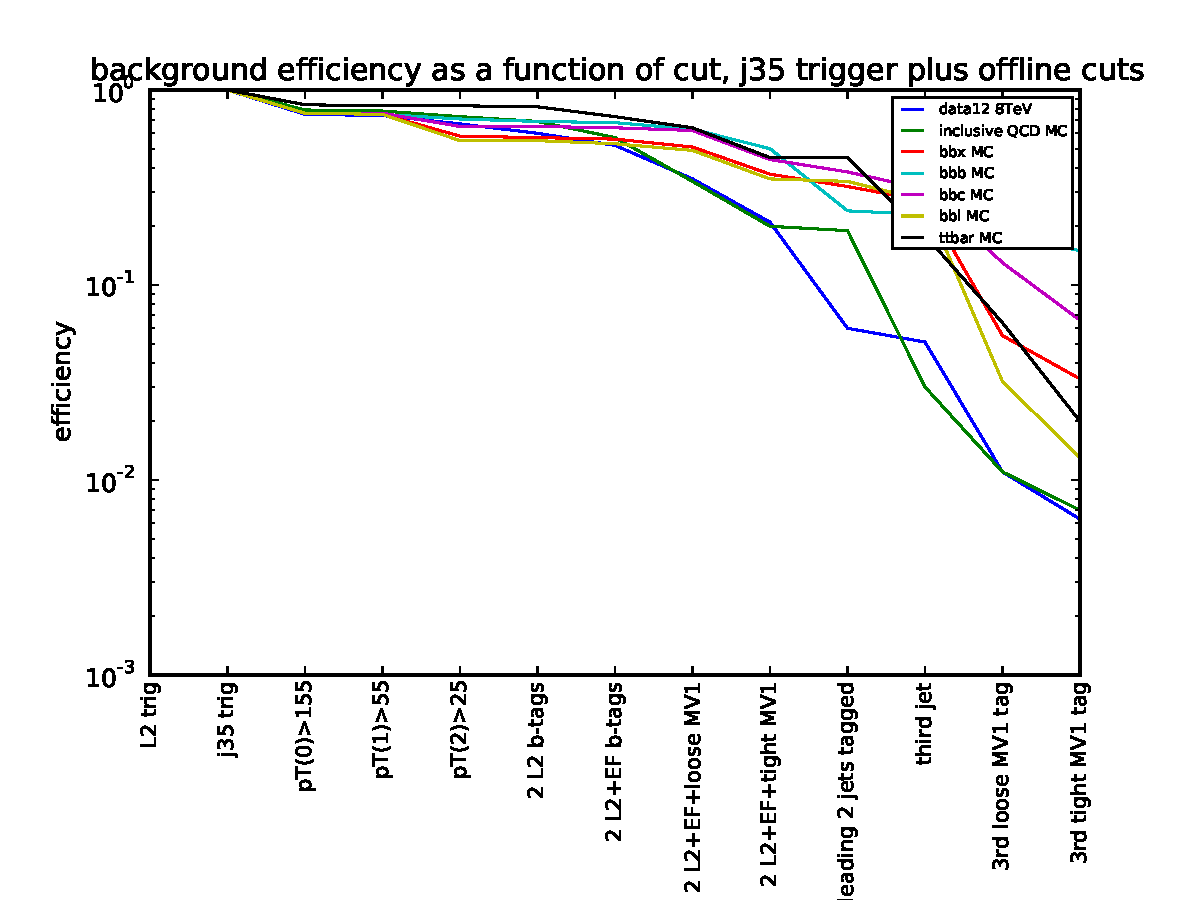
\includegraphics[width=0.45\textwidth]{TriggerCuts/cut_efficiencies_logy_j35_background.pdf}	
    \caption{The cut efficiencies in background, cut by cut. The background component that has 
    three real $b$-jets from QCD has the greatest survival rate through the cut flow, followed
    by events that have two $b$-jets and one $c$-jet.\label{fig:background_eff_cutflow}}
\end{figure}

%------------------------------------------------------

%------------------------------------------------------
\begin{figure}
    \center
	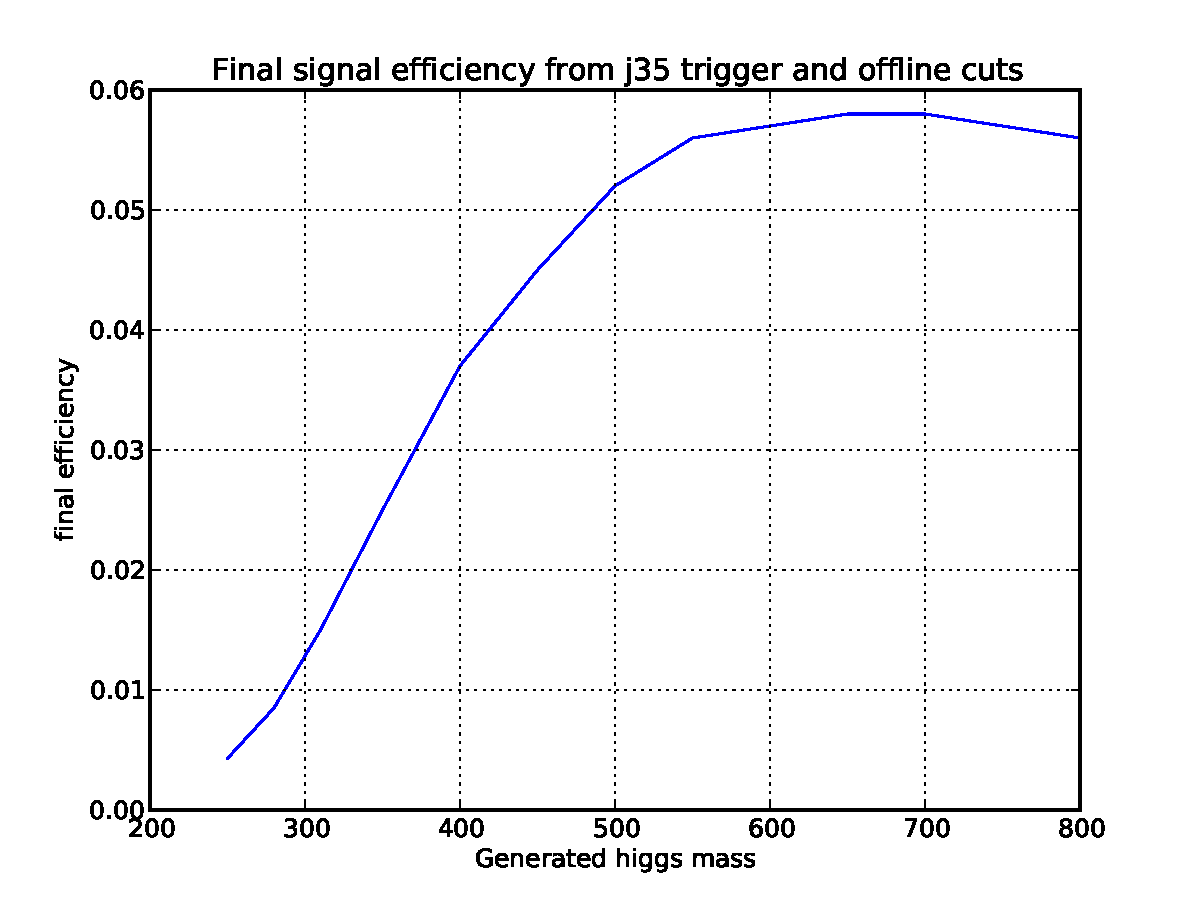
\includegraphics[width=0.6\textwidth]{TriggerCuts/final_efficiency_vs_mass_j35.pdf}	
    \caption{The final efficiency, after all cuts, of the signal as a function of
    the physical mass of the generated Higgs particle.  The signal efficiency grows as a
    function of $m_A$, although at the high mass values, the efficiency levels off at around 6\%.\label{fig:final_eff_vs_mass}}
\end{figure}

%------------------------------------------------------









% Activate the following line by filling in the right side. If for example the name of the root file is Main.tex, write
% "...root = Main.tex" if the chapter file is in the same directory, and "...root = ../Main.tex" if the chapter is in a subdirectory.
 
%!TEX root =  ../Thesis.tex

\chapter[Background Estimation]{Background Estimation}

Once the background has been reduced as much as practical using the trigger and kinematic cuts,
a reliable estimate of the shape and size of the remaining background is critical to optimizing
the exclusion limits.  As detailed in Section~\ref{sec:mass_res}, since the reconstructed mass peak 
of the leading two $b$-jets is so
broad in signal, a mis-estimation of the background shape can lead to systematic errors that
could wash out any possible signal (or worse, be mistaken for a signal where there is none).  

At the same time, the backgrounds in this analysis are challenging to estimate, either in Monte
Carlo simulations or using data-driven methods.  Therefore, much of the work of this analysis is dedicated
to validating the background, especially its shape in jet $p_T$, $m_{bb}$, and so on.



\section{Background Estimation Strategy}
\label{sec:background_strategy}
As QCD is the dominant background in this analysis, it is important to understand
what flavors of QCD jets compose the population of events that survive the cut
chain.  In order to do this, we apply the trigger and cut chain detailed in Chapter~\ref{chap:trig_cuts}.

Once the events have been passed through the cut chain, 
the signal and background are split into 3 exclusive regions based on the $b$-tag weight of the
third jet in the event\footnote{as noted below, the ``third jet'' moniker does not strictly
mean the third-highest $p_T$ jet in the event; rather, it is the jet with the highest $b$-tag weight
that is \textit{not} one of the leading two jets in $p_T$, which are already $b$-tagged coming
out of the cut chain}:
\begin{itemize}
    \item \textit{bbb}: one or more jets (in addition to the two triple-tagged jets) passing a tight (60\% $b$-jet efficiency working point)
 MV1\footnote{recall that MV1 is the name of the offline $b$-tagging algorithm used in most ATLAS analyses} cut
    \item \textit{bbloose}: events failing the \textit{bbb} classification but which have one or more jets passing a loose (80\% efficiency
 working point) MV1 cut
    \item \textit{bbanti}: events that have no jets passing an 80\% MV1 cut-–effectively a veto on the presence of any
 $b$-tagged jets other than those firing the trigger
\end{itemize}

When assigning events to one of these categories, we only allow $b$-tags on the leading
five jets to count toward the $bbb$ or $bbloose$ categories.  In other words, if the third
$b$-tagged jet in an event is the 6th jet (in $p_T$ ordering) overall, the event 
will be classified as $bbanti$.  This requirement is motivated by our physics awareness that
the $b$-jets coming from signal events should be fairly high $p_T$, so this should have
a minimal effect of rejecting signal that would otherwise be accepted.  On the other
hand, with high-jet-multiplicity QCD events, there is the combinatorial effect of looking across
more jets for $b$-tags that increases the likelihood of an event being classified as signal-like
(\textit{bbb} or \textit{bbloose}) as there are more jets in the event.  Only looking at the leading 5 jets
for $b$-tags keeps this effect under control. 

Once all the events have been categorized, the search proceeds by fitting the background
in the \textit{bbanti} region, which we sometimes refer to as the \textit{bbanti}
control region.  The events in this category will be mostly QCD background, especially
$b\bar{b}$ QCD, although about 20\% of the signal might fall into this category.  The 
\textit{bbb} category will be enriched in $b\bar{b}b$ events, either from signal
or QCD background, although 60\% of the signal falls into this category and the QCD 
backgrounds are much lower when a third $b$-jet is required.  The background estimation
strategy for this analysis is to fit the $m_{bb}$ distribution in the background-dominated
\textit{bbanti} category, and use that shape to predict the background shape in the \textit{bbb}
signal region.   The extrapolation from \textit{bbanti} to \textit{bbb} is validated using the 
bb QCD MC sample described in Section~\ref{sec:bb_qcd_mc}.

\section{Background Estimation Method Based on Parameterized Histogram Fitting}
The background consists almost exclusively of QCD with 2 or more real $b$-jets, which 
fortunately has a $m^{'}_{bb}$\footnote{the $m^{'}_{bb}$ variable is described in more detail
immediately below, and in Section~\ref{sec:rotation}} spectrum that does not have any peaks or other difficult
structure above about 350 GeV.  Below that mass, the trigger turn-on curve becomes
a major feature of the spectrum.  Above that mass, there
is a smoothly falling distribution that we fit to an RhhBinnedPdf, which is a parameterized
histogram PDF (probability distribution function) that is also used for fitting the signal.

In a few words, the background fit strategy proceeds in the following way:
\begin{itemize}
    \item Start with a signal mass point
    \item Apply a mass-point-specific rotation based on the the eigenvectors of 
    the signal MC sample of that mass point, as calculated using $m_{bb}$, $p_{T,1}$ and $p_{T,2}$; we call 
    the components of this rotated basis $m_{bb}'$, $p_T^{1'}$ and $p_T^{2'}$ (more
    details in Section~\ref{sec:rotation}).  Briefly, the $m^{'}_{bb}$ variable
    is a linear combination of $m_{bb}$, $p_{T,1}$ and $p_{T,2}$, which has a shape
    similar to $m_{bb}$ but exploits correlations in the signal to suppress the backgrounds.
    \item Apply cuts to $p^{'}_{T,1}$ and $p^{'}_{T,2}$, and use $m_{bb}^{'}$ as the final 
    discriminating variable 
    \item Fit the $m_{bb}^{'}$ distributions within the $m^{'}_{bb}$ ranges specified in Table~\ref{tab:mass_window} 
    with a parameterized histogram, separately for each $b$-tag and $n_{jets}$ category
    in signal MC.
    \item Fix the signal shapes and relative category normalizations to the fits found in MC
    \item Create a composite PDF that is the sum of the signal PDF and a background PDF; 
    the background PDF is not yet known (either shape or normalization) but the model is a
    parameterized histogram, with the same range and binning as the signal fits.  

    \item Fit the data in the same $m_{bb}^{'}$ range, also with a parameterized histogram.
    The fit is a simultaneous fit to the data in the 
    $bbb$, $bbloose$, and $bbanti$ tag
    categories\footnote{a simultaneous fit will find the parameters that maximize the likelihood
    across all three tag categories; in other words, the shapes of the background in these three
    tag categories are found during this step of the fit}.
    For example, all 3-jet events (whether in the
    $bbb$, $bbloose$, or $bbanti$ tag category) are fit with nearly the same histogram in data (details below).
    This has the practical effect of $bbanti$ dominating the fit result because of its
    higher statistics, so the resulting
    histogram is dominated by the $m_{bb}^{'}$ distribution in background tag categories.
    \item For the background PDF, incorporate a parameter into the fit that allows the $bbb$,
    $bbloose$, and $bbanti$ distributions to vary by a linear function with a slope that is
    found by the fit.  This allows for linear differences in the shapes of the $m^{'}_{bb}$ distribution
    depending on $b$-tag category, which we observe when studying background MC simulations.
    \item Allow the overall signal normalization to float in the final fit (not, however, the relative normalization
    between categories or the signal shapes) so that, while the background shape will be
    dominated by the signal-depleted $bbanti$ region, the $bbb$ region in particular can
    have contributions from signal.
    \item Solve for the signal cross section, background shape, background linear variation
    between tag categories, and background normalization
    that maximizes the total likelihood across
    all tag categories simultaneously.
%    \item Create a composite PDF that is the sum of the background and signal components
%    \item Initialize the parameters of the background component to the final parameter values
%    found in the background-only fit, but allow the background parameters to float in 
%    the fitting procedure
%    \item Fit the data in the signal region, allowing the background shape, background
%    normalization, and signal normalization to float
    \item Repeat for the next signal mass point
\end{itemize}

Although we have signal MC with $m_A$ values as low as 250 GeV, this fit strategy only
begins to work above $m_A=$400 GeV, because of the trigger turn-on curve.  The signal mass 
points to which we would have sensitivity range from 450 to 800 GeV (potentially higher,
but 800 GeV is our highest signal MC point). 

While the analysis was in development, it was blinded to avoid bias.  This was done 
by removing \textit{bbb} events from the data, and replacing them with a sample of
events with the same normalization drawn from the \textit{bbanti} distribution
in data.  For the final search, the \textit{bbb} events were substituted back in.



%\section{Turn-On Curve Modeling}
%Although the lowest part of the $m_{bb}$ distribution (below 300 GeV) is not part of the search regime,
%because of the rapidly changing background, including it in the background model helps
%improve the overall fit by allowing for a slightly fewer events at moderately low
%$m_{bb}$ (between about 300 and 400 GeV) than an exponential alone would predict.
%The turn-on is fit with a logistic function of the form

%\begin{equation}
%f(m_{bb}) = N\frac{1}{1+e^{-c(m_{bb}+d)}}
%\end{equation}

%In this equation, N controls the overall normalization, $c$ governs the steepness
%of the turn-on curve, and $d$ is the horizontal offset.

%\textbf{once we confirm this (or something like it) as the final fit model,
%add a plot showing how this function changes with c/d and the composite
%model of exponential times logistic}


\section{Modeling of Background Shape}
\subsection{Selection of Parameterized Histogram}
Once the rotation and cuts have been applied, the data is fed into an 
binned maximum likelihood fit for mathematical modeling.  The fitting
of both signal and background is done in RooFit.  There are a number 
of candidate models for the background fit, which can be evaluated
both on their goodness-of-fit (as measured by a metric like $\chi^2/DOF$)
and their ease of convergence.

A number of mathematical functions were attempted in fitting the
background, but in the final analysis, a parameterized histogram was
used in part because of its easier convergence on background, and
in part it allowed us to avoid an unstable functional fit to the signal.

The important compromise of fitting to a histogram for the
background is that it removes some of the constraints that a functional
fit provides (for example, a decaying exponential imposes the constraint
that the background is always decreasing as $m^{'}_{bb}$ increases, 
but a histogram could fluctuate up in the case of an excess).  That 
means that we must rely on our background-dominated $bbanti$ region
to understand the shape of the background, and then extrapolate that
shape to the $bbb$ signal region in order to look for deviations from
the background-only hypothesis.  

%The extrapolation must be validated in 
%background MC: the assumption this method makes is that the $m^{'}_{bb}$
%distribution is the same regardless of the flavor of the third jet 
%in the event.  If that assumption holds, this extrapolation method is a
%valid way to predict the background shape in the signal region.


The PDFs for $m^{'}_{bb}$ are based on a parameterized step function,
which is equivalent to parameterizing a normalized histogram in terms of the content of each
bin. The number of needed parameters correspond to the number of bins minus one
(because of the normalization). Using directly the bin content in each bin
$b_{i}$ would induce an unstable behavior, since the last bin
content would need to be parameterized as $1-\sum_{i=1}^{(N_{bins}-1)} b_{i}$
and the fit would easily converge to configurations where the last bin is negative,
and at that point convergence is spoiled. Instead, the values of $p_{i}$
are re-parameterized in terms of another set of parameters
$b_{i}$\footnote{This nice trick was introduced for the first time by Aaron Roodman (SLAC) in the BaBar experiment}.

\begin{itemize}
\item $b_{1} = p_{1}$
\item $b_{2} = p_{2} \left(1-p_{1}\right)$
\item $b_{3} = p_{3} \left(1-p_{2} \right) \left( 1-p_{1}) \right)$
\item $....$
\end{itemize}
With this choice all parameters $p_{i}$ with $i$ from 
1 to $N-1$ can be limited to $[0,1]$, without loss of generality, 
and the fit will always converge reliably, provided the dataset the fit is applied 
to has at least one event in each bin of the PDF.

As we have described it so far, the background fit makes the assumption of the
same background shape in the $bbb$, $bbloose$ and $bbanti$ tag categories.
However, from studies in background MC simulations, we suspect that there may 
be relatively small systematic shape differences in the different tag
categories, and those shape differences are linear in the ratio of the $m^{'}_{bb}$
distributions in $bbb$ and $bbanti$ (also $bbloose$ and $bbanti$; for more
details on these background MC studies, see Section~\ref{sec:background_syst}).
Although these shape differences are small compared to the overall shape of the
$m^{'}_{bb}$ distributions, the difference can be comparable to the effect from
a possible signal.  In order to account for this, we add an additional parameter
to the fit, which allows for a linear variation on the ratio of $m^{'}_{bb}$
between the different tag categories.  The value of this parameter is found
during the fitting process; it is constrained to [-1, 1] where -1 corresponds to
reducing the contents of the first bin to approximately zero and doubling the contents
of the last bin, while +1 does the opposite.


%of that can vary between the 
%tag categories and account for shape differences.


In the final fit to the data sample the following parameters are extracted:
\begin{itemize}
\item The signal strength $\mu$;
\item The background normalizations $N_{bkg,l}$, separately in each category;
\item The background $PDF_{bkg}(m_{bb})$, which is constrained to the same shape in all
tag categories aside from a possible linear variation allowed between various tag categories; and
\item The size and sign of linear variation in the $m^{'}_{bb}$ distribution from tag category to tag category 
\end{itemize} 


Although the final fit model was a histogram, the following functions were
also considered and we discuss below the behavior they exhibited:
%In brief, the functions given consideration include the following:
\begin{itemize}
    \item Bernstein Polynomial
    \item Power Decay Series
    \item Decaying Exponential with 1 parameter
    \item Decaying Exponential with 2 parameters
\end{itemize}

\subsubsection{Bernstein Polynomials}
The Bernstein polynomials are a family of polynomials that are characterized
particularly by their attractive feature of being positive-definite, or never
predicting a negative value for a PDF composed of them.  However, we find
that it takes a high degree of polynomial (5 parameters or more) to fit the
background over the full mass range, and a polynomial with a 
degree this high struggles (and often fails) to converge.  Moreover, a
drawback of high-degree polynomials is their capability to ``wiggle'' and
potentially absorb a signal within the background model.

\subsubsection{Power Decay Series}
A power decay series of the form $\frac{a}{x} + \frac{b}{x^3} + \frac{c}{x^5} + ...$
is another possibility; if all the powers of $x$ in the denominators are
odd, this series cannot wiggle like the Bernstein polynomials.  However,
a simple series with a few terms does not fit the background shape well 
over the full mass range, and when many terms are added to the series then
the fit struggles to find a global maximum of the likelihood function, leading
to non-convergence.

\subsubsection{Decaying Exponential with 1 Parameter}
Like a decaying power series, a decaying exponential function is monotonically
decreasing; however, unlike a power series, an exponential with a single
parameter (i.e. a model of the form $f(x)=e^{-x/\tau}$) provides 
a relatively good fit to the background distribution in most tag and jet
categories, with $\chi^2/DOF$ values below 2 for all \textit{bbb} and \textit{bbloose}
distributions \footnote{the \textit{bbanti} distributions prove harder to
fit with a 1-parameter exponential, with $\chi^2/DOF$ values between 2.8 and 3.9}.
Additionally, the simplicity of a 1-parameter exponential means that the
fits converge quickly and reliably over the full mass range.

\subsubsection{Decaying Exponential with 2 Parameters}
A decaying exponential with two parameters (i.e. a model of the form  $f(x)=e^{-x/\tau+\omega x^2}$)
has some of the same nice features of a single-parameter exponential (simple functional
form, no possibility of signal-spoofing wiggles) while offering
more flexibility than the 1-parameter exponential.  The $\chi^2/DOF$ and pulls
for the 2-parameter exponential fits reflect this flexibility to better
fit the data, every jet/tag category has a fit that is as good or better
for the 2-parameter exponential as for the 1-parameter exponential.  In 
particular, the \textit{bbanti} categories that have higher $\chi^2/DOF$ values
in the 1-parameter fit show $\chi^2/DOF$ results of 1.0-1.2 with the 2-parameter fits. 
However, the convergence of this model (especially when it is used in a composite
model that can also include signal) can be tricky, and we found that in practice
the parameters need to be initialized and constrained very precisely to get
good results.  We also found that this model was prone to introducing spurious
signal when used in combination with our signal, so that even when running in 
configurations where no signal was present, the fit was prone to returning
a nonzero signal cross section.


%%% START HERE


\subsection{Validation of Background Shape Extrapolation}
A critical assumption of this fit method is that the shape of the $m_{bb}$ distribution
varies only linearly based on the flavor (or, relatedly, $b$-tag status)
of the third jet in the event.  We validate this assumption in the $b$-jet enriched 
QCD MC sample detailed in Section~\ref{sec:bb_qcd_mc}

As detailed in Section~\ref{sec:rotation}, our final discriminating variable is actually
not $m_{bb}$ but a variable we call $m_{bb}^{'}$, 
which is a linear combination of $m_{bb}$, $p_{T,1}$ and $p_{T,2}$.  So while we
do check that the $m_{bb}$ distributions are not biased by the flavor of the third jet,
the real figure of merit lies in showing that $m_{bb}^{'}$ is not biased by the
flavor of the third jet either.  The plots in Figure~\ref{fig:bkg_shape_compare}
show $m_{bb}^{'}$ in the $bbb$ and $bbanti$ tag categories, with a ratio plot drawn below
to see any shape differences more clearly.  


%Although not all the bins agree 
%exactly between the \textit{bbb} and \textit{bbanti} categories, there is little sign of a bias in the 3-jet
%or 4-jet categories; the 5-jet category shows a slight shape difference at high values
%of $m_{bb}^{'}$ for which we assign a systematic error (more details in Section~\ref{sec:background_syst}).

\begin{figure}[hbt]
\center
\includegraphics[width=0.45\linewidth]{BackgroundEstimation/mbb_bbb_3jets_rotated.pdf}
\includegraphics[width=0.45\linewidth]{BackgroundEstimation/mbb_bbb_4jets_rotated.pdf}
\includegraphics[width=0.45\linewidth]{BackgroundEstimation/mbb_bbb_5jets_rotated.pdf}
\caption{The distributions of the final discriminating variable, $m_{bb}^{'}$, 
in background MC for the $bbanti$ and $bbb$ tag categories.  The three different plots
compare the 3-jet, 4-jet, and 5-or-more jet categories.  No signs of major shape
differences are seen.
\label{fig:bkg_shape_compare}}
\end{figure}

A fuller suite of plots can be found in the Systematics Chapter, Section~\ref{sec:background_syst}.
In these plots, we fit linear functions to the ratios, and find that especially in the 
5+ jets category, the shape can vary by a statistically signficant amount.  

We use the background MC simulations to verify that the fit, as written, can correctly
account for linear shape differences from tag category to tag category.  We manually apply
linear shape variations to the $bbb$ tag category, relative to $bbanti$, and send the 
resulting distributions through the fitting infrastructure to verify that the parameters
reflect the presence of the variations.  We find that the fit correctly accounts for the 
variations, and that the background shapes found by the fit agree perfectly with the distributions
that were fed into the fit.






 


%Following the prescription in the Standard Model $h\rightarrow\gamma\gamma$
%search \cite{spurious_signal}, the model must meet at least one of the following
%criteria:

%\begin{itemize}
%    \item $N_{sp}<$ 10\% $N_{s,exp}$
%    \item $N_{sp}<$ 20\% $\sigma_{bkg}$
%\end{itemize}

%$N_{s,exp}$ is the number of signal events expected to pass the event selection cuts, and 
%$\sigma_{bkg}$ is the statistical uncertainty on the number of background events when
%fitting the signal+background model to the background-only Asimov dataset.

%\textbf{fill in results of these tests after they have been completed}


\subsection{Non-QCD Background}
\label{sec:non_qcd_bkgs}

\subsubsection{All-Hadronic $t\bar{t}$ Background}
When $t\bar{t}$ decays all-hadronically, it can create events with several high-$p_T$
jets and two or more $b$-tagged jets (where the $b$-tags come from both real $b$-quarks
and from mistagged light flavor).  We anticipate that, because it has a production
cross section that is much smaller than QCD\footnote{this statement depends somewhat
on cuts, $b$-tagging, etc., but as explained below it does turn out to be the case
in the relevant region in phase space for this analysis}, $t\bar{t}$ will not be a major background.
%We confirm this assumption in MC by using the all-hadronic $t\bar{t}$ sample summarized
%in Table~\ref{tab:ttbar_params}.


%\begin{deluxetable}{cccc}
%\tablewidth{0pc}
%\tablecolumns{4}
%\tablecaption{Parameters of the $t\bar{t}$ MC sample used in this analysis. \label{tab:ttbar_params}}
%\tablehead{
%    \colhead{Dataset ID} & \colhead{Cross Section [nb]} & \colhead{Filter Efficiency} & \colhead{N Events}  }
%    \startdata
%    117050 & 0.21085 & 0.54298 & 99930891 \\
%    \enddata
%\end{deluxetable}


We find that in Pythia MC simulations, all-hadronic $t\bar{t}$ has an efficiency of 7.5\% after
the EF\_2j35\_loose\_j145\_j35\_a4tchad trigger, and approximately 2\% efficiency
in the offline cuts relative to the trigger.  Estimating the $t\bar{t}$ cross section
as 165 pb, and a 44\% branching ratio in the all-hadronic decay channel, this gives
a 0.11 pb $t\bar{t}$ cross section expected after the trigger and offline cuts.  In the
full 2012 dataset, this amounts to about 2400 events.  While
this is not a negligible cross section compared to the signal, it is more than an
order of magnitude smaller than the QCD background.

In addition to checking the magnitude of the $t\bar{t}$ background, we check the shape
for any shape differences in the $m_{bb}$ distribution depending on the tag status of the
third jet, and do not find any major discrepancies that point toward $t\bar{t}$ as a
potential peaking background in the signal region. The $m_{bb}$ distributions in the
bbb, bbloose and bbanti bins for the all-hadronic $t\bar{t}$ can be found in Figure
~\ref{fig:ttbar_mbb}.




\begin{figure}[hbt]
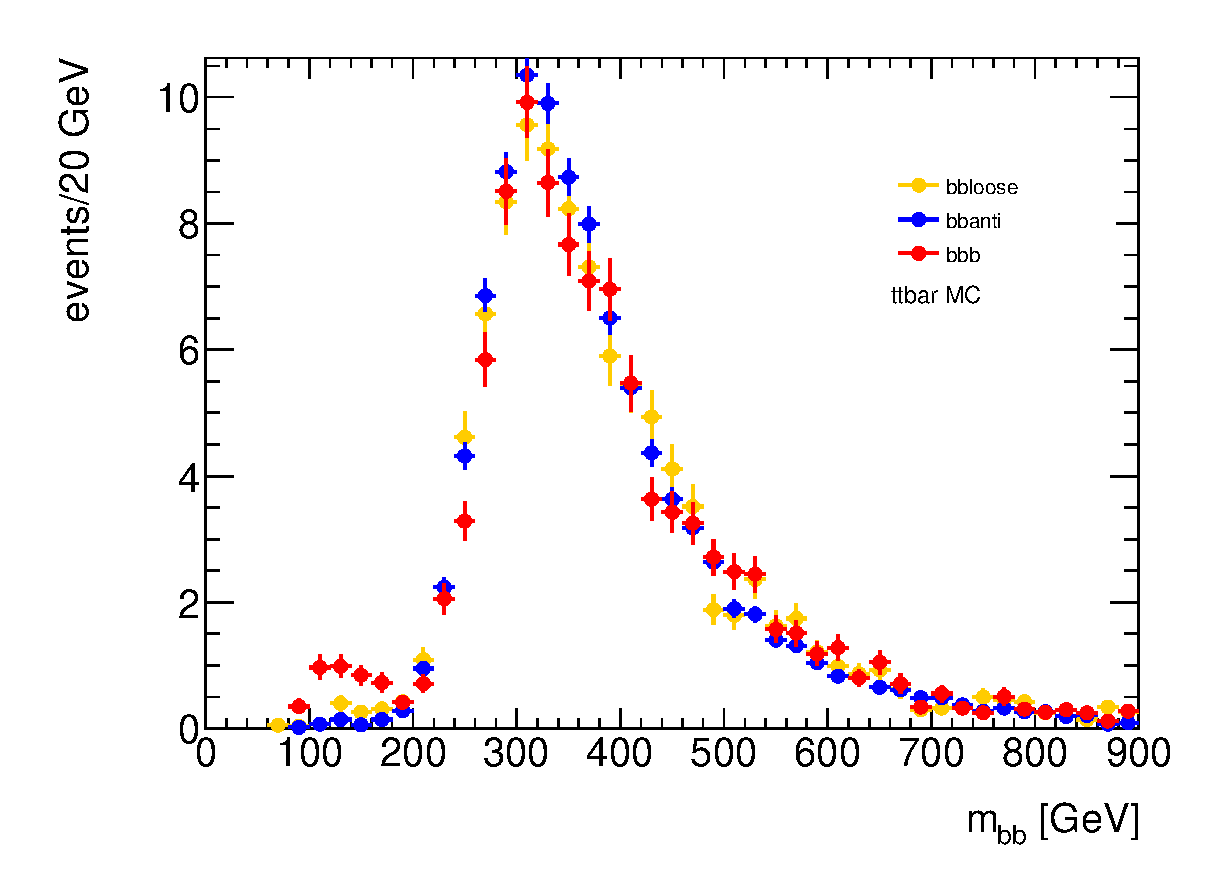
\includegraphics[width=0.45\linewidth]{BackgroundEstimation/images/mbb_compare_bbb_bbloose_bbanti_ttbar.eps}
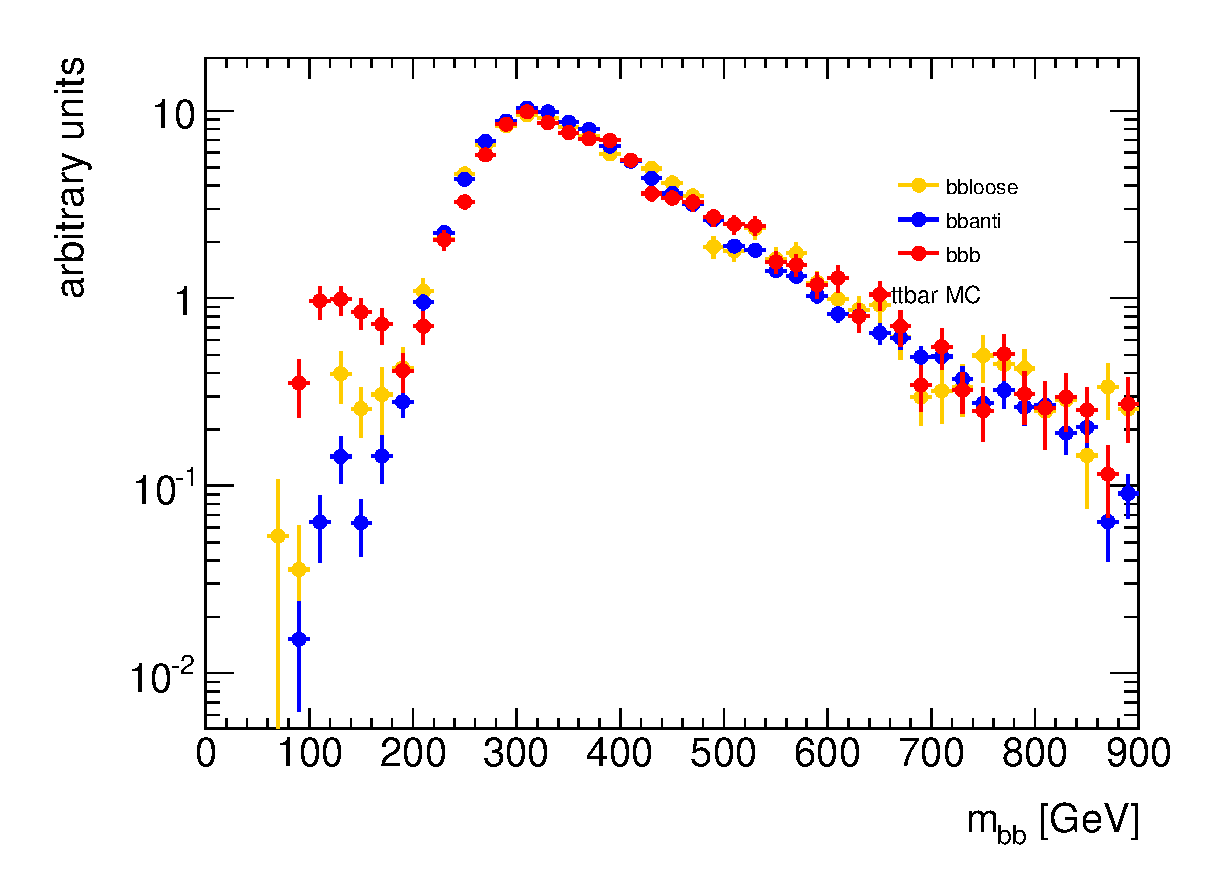
\includegraphics[width=0.45\linewidth]{BackgroundEstimation/images/mbb_compare_bbb_bbloose_bbanti_ttbar_logy.eps}
\caption{The $m_{bb}$ distributions for all-hadronic $t\bar{t}$ MC after the trigger and all offline cuts are applied (linear Y axis on the left, logarithmic scale on the right).  In addition to the overall cross-section, we also want to probe any shape differences that arise when the tag status changes on the third jet in the event.  No significant shape differences are seen.}
\label{fig:ttbar_mbb}
\end{figure}



















% Activate the following line by filling in the right side. If for example the name of the root file is Main.tex, write
% "...root = Main.tex" if the chapter file is in the same directory, and "...root = ../Main.tex" if the chapter is in a subdirectory.
 
%!TEX root =  ../Thesis.tex

\chapter[Signal Kinematics]{Signal Kinematics}
 
\section{Signal Jet Kinematics}

\section{Signal Jet Combinatorics}

\section{Mass Resolution}
Once the trigger and all the analysis cuts have been applied, we take the leading 2 jets in the event (which are also the leading 2 $b$-tagged jets, since we place a cut requiring that the leading 2 jets in the event be $b$-tagged) and reconstruct their combined invariant mass--if they came from a decaying particle, the reconstructed mass should be the mass of the parent particle.  On the other hand, if the leading 2 jets come from continuum QCD processes, there should be no resonance present, so we look for the presence of a resonance peak on top of a decaying power-law background.

The sensitivity of this analysis depends on the signal cross section and efficiency, the background cross section and efficiency, but also the signal resolution.  The broader the signal mass peak, the more difficult it is to distinguish from the background.  

Unfortunately, the mass resolution significantly degrades as a $m_A$ grows.  Some of this is due to the inherent width growing as $m_A$ grows, as can be seen in Table~\ref{tab:sig_mc_parameters}.  

\subsection{Mass Resolution Improvement after Requiring that Leading Two Jets be $b$-Tagged}
The mass resolution also improves when we require that the leading two jets in the event be b-tagged;
 the plots in Figure 39 and Figure 40 show the ect on the invariant mass distribution.
 In order to quantify the mass resolution ect, we define the “left” and “right” shoulders of the mbb
 distribution, which are respectively the portion of the mbb distribution that are below and above the peak.
 go into further detail on the signal shape in Section 6.2; but in Table~\ref{tab:signal_mass_RMS_compare} the RMS of especially the left
 shoulder before and after requiring b-tags on the leading 2 jets quantitatively shows the mass resolution
 improvement.



%----------------------------------------------
\begin{table}
\centering
\caption{The RMS of the mass distribution in the left and right shoulders of the peak,
    as explained in the text.  The left shoulder is dominated by radiation off the Higgs
    and/or the Higgs daughter jets in addition to combinatorial mis-reconstructions,
    leading to a larger RMS than the right shoulder, which
    is dominated by combinatorics only.\label{tab:signal_mass_RMS_compare}   }
  \begin{tabular}{ccccc}
     \hline \hline
     generated mass (GeV) & \multicolumn{2}{c}{require $b$-tags on leading 2 jets (GeV)} & \multicolumn{2}{c}{no $b$-tag required on leading 2 jets (GeV)}  \\
        & left & right & left & right \\ \hline
     250 & 13.5 & 89.2 & 36.7 & 87.7 \\
     280 & 19.2 & 68.8 & 27.5 & 71.4 \\
     310 & 19.2 & 58.3 & 31.8 & 58.1 \\
     350 & 28.3 & 34.5 & 33.9 & 36.2 \\
     400 & 33.4 & 26.1 & 45.1 & 26.5 \\
     450 & 39.5 & 25.7 & 62.2 & 25.9 \\
     500 & 48.6 & 29.3 & 81.1 & 29.8 \\
     550 & 54.9 & 31.1 & 93.1 & 33.3 \\
     600 & 73.0 & 26.0 & 117.6 & 30.5 \\
     650 & 75.4 & 31.7 & 130.8 & 31.8 \\
     700 & 75.7 & 40.3 & 143.4 & 40.7 \\
     800 & 100.9 & 36.2 & 177.4 & 36.3 \\
     \hline     \end{tabular}
\end{table}
%----------------------------------------------


%----------------------------------------------
\begin{figure}
    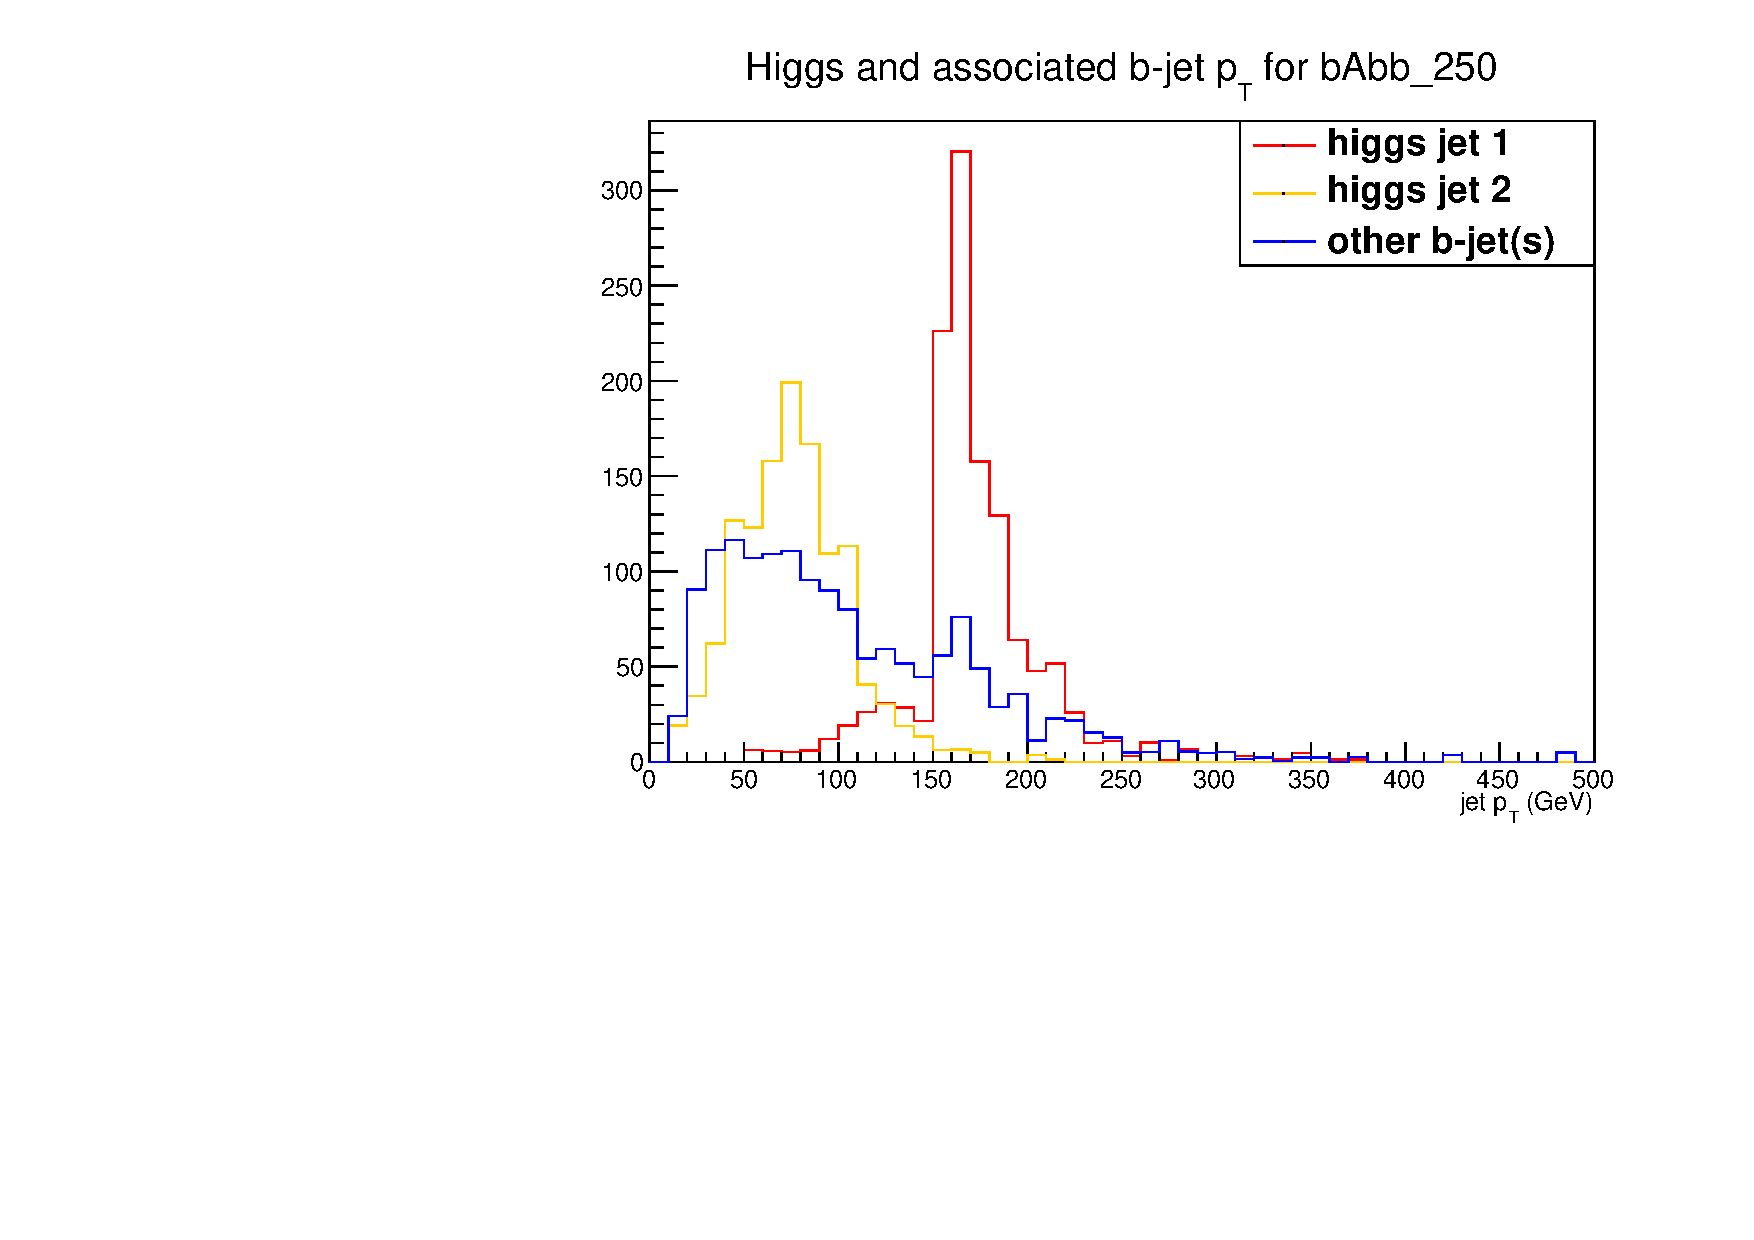
\includegraphics[width=0.33\textwidth]{/Users/caitlinmalone/Documents/Thesis/SignalKin/jet_pt_compare_bAbb_250.pdf}
    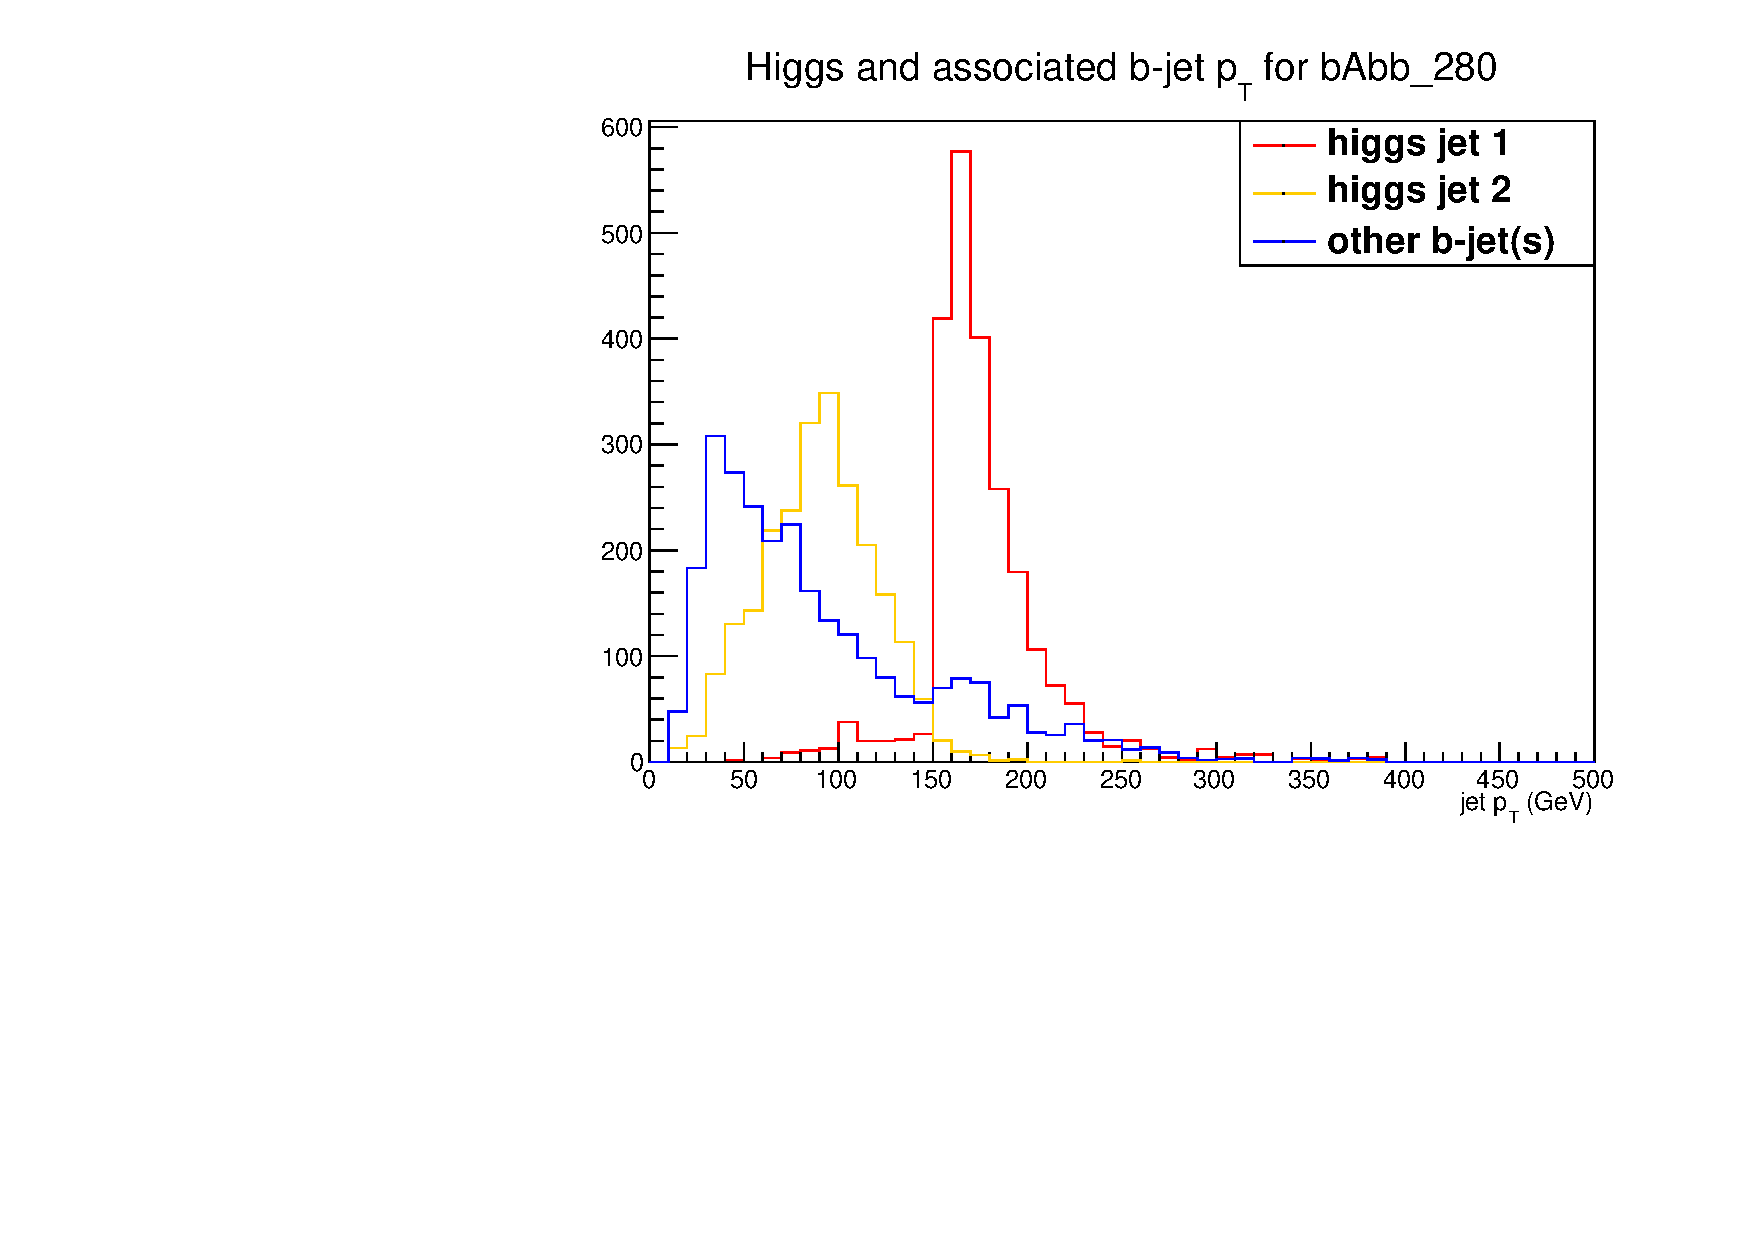
\includegraphics[width=0.33\textwidth]{/Users/caitlinmalone/Documents/Thesis/SignalKin/jet_pt_compare_bAbb_280.pdf}
    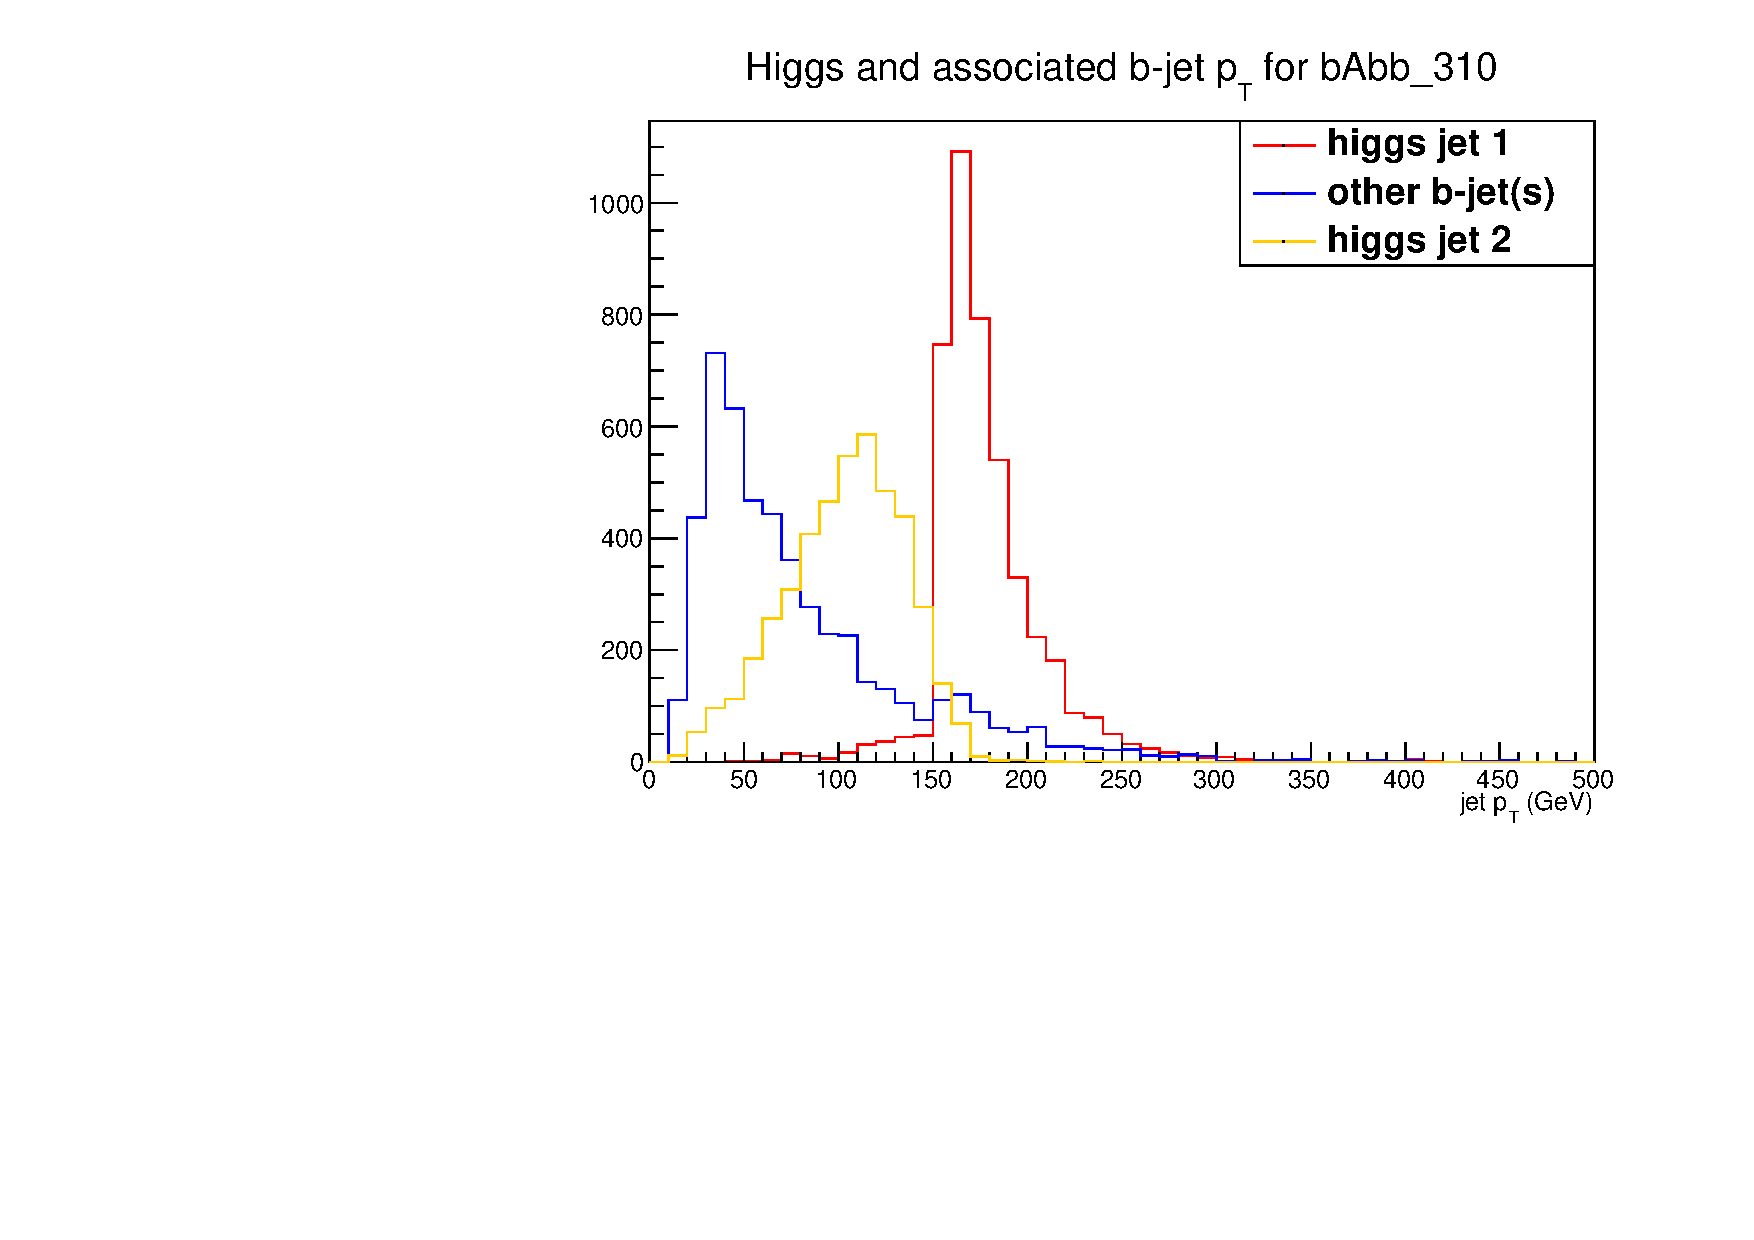
\includegraphics[width=0.33\textwidth]{/Users/caitlinmalone/Documents/Thesis/SignalKin/jet_pt_compare_bAbb_310.pdf}
%    \newline
    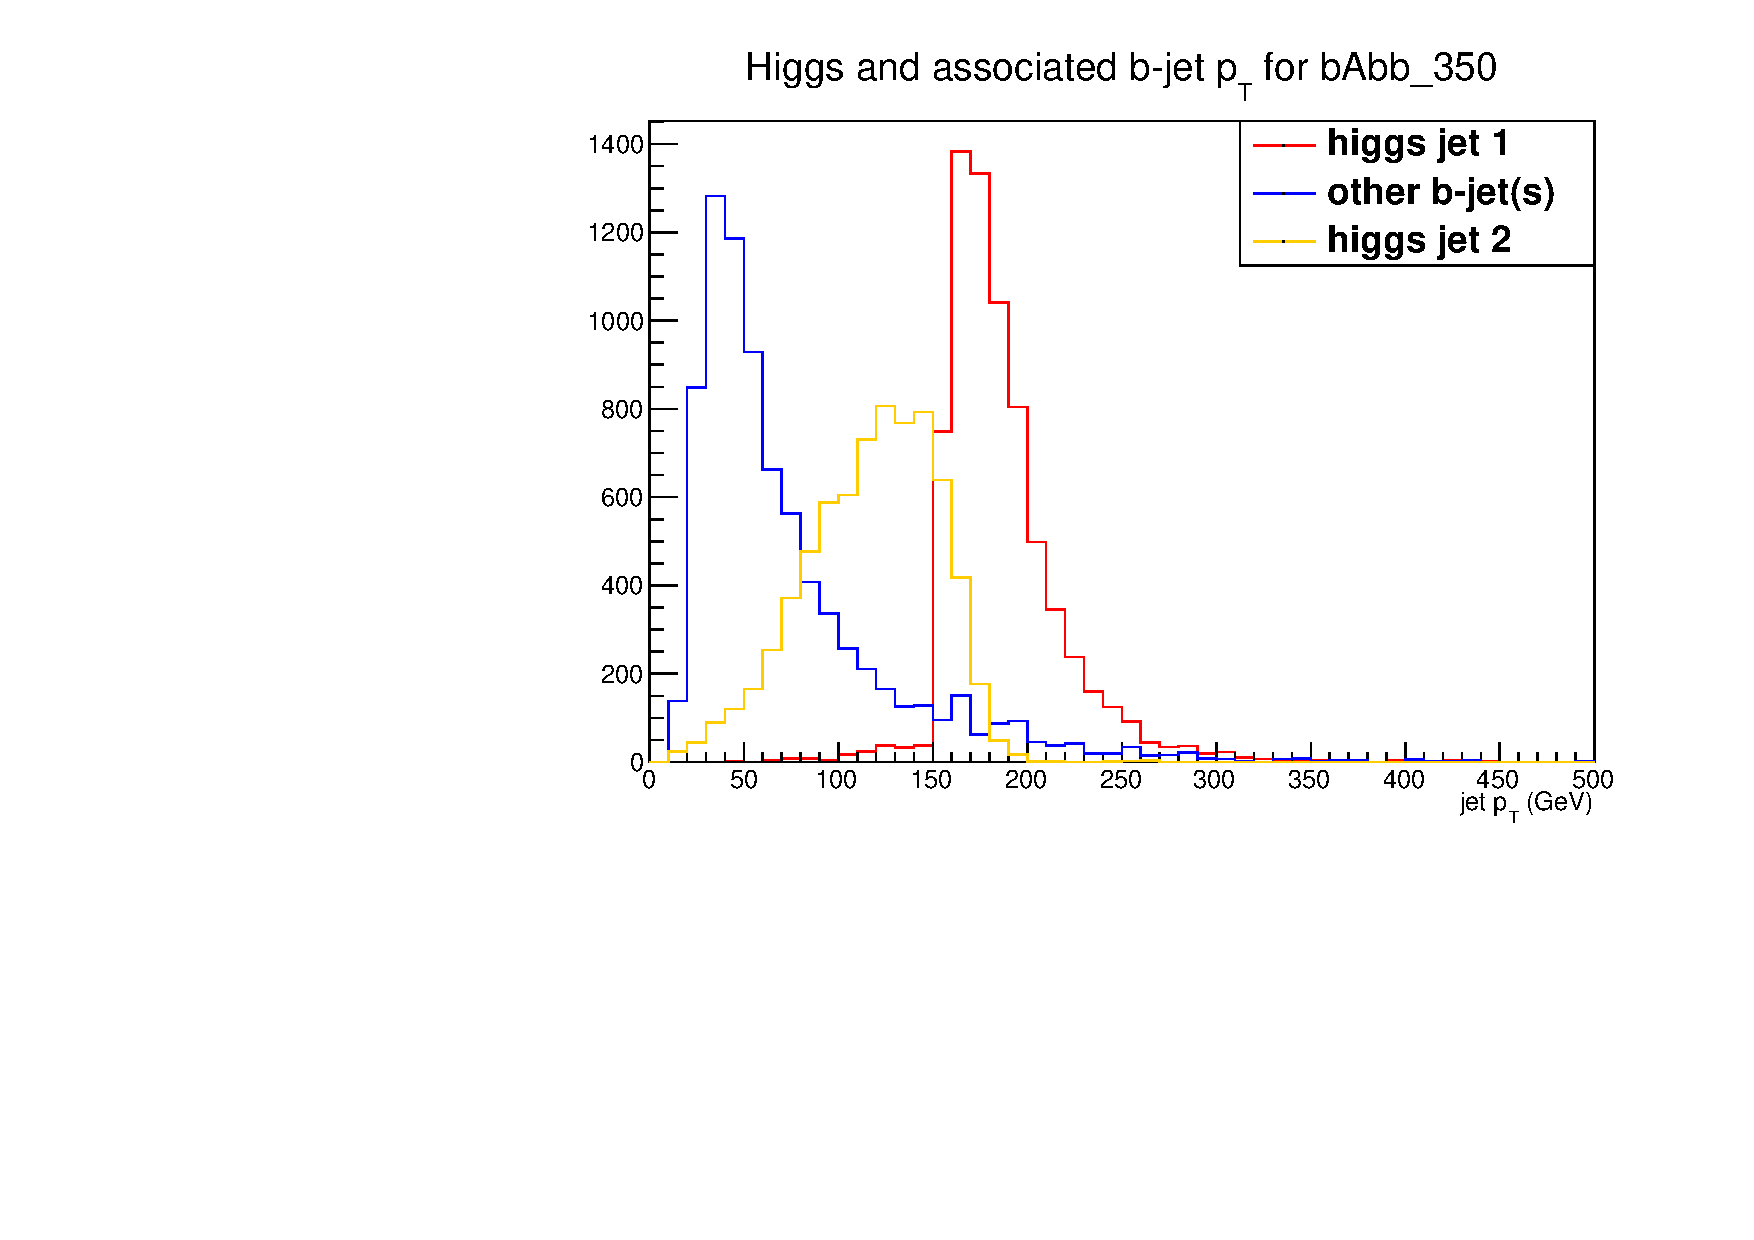
\includegraphics[width=0.33\textwidth]{/Users/caitlinmalone/Documents/Thesis/SignalKin/jet_pt_compare_bAbb_350.pdf}
    \includegraphics[width=0.33\textwidth]{/Users/caitlinmalone/Documents/Thesis/SignalKin/jet_pt_compare_bAbb_400.pdf}
    \includegraphics[width=0.33\textwidth]{/Users/caitlinmalone/Documents/Thesis/SignalKin/jet_pt_compare_bAbb_450.pdf}
%    \newline
    \includegraphics[width=0.33\textwidth]{/Users/caitlinmalone/Documents/Thesis/SignalKin/jet_pt_compare_bAbb_500.pdf}
    \includegraphics[width=0.33\textwidth]{/Users/caitlinmalone/Documents/Thesis/SignalKin/jet_pt_compare_bAbb_550.pdf}
    \includegraphics[width=0.33\textwidth]{/Users/caitlinmalone/Documents/Thesis/SignalKin/jet_pt_compare_bAbb_600.pdf}
%    \newline
    \includegraphics[width=0.33\textwidth]{/Users/caitlinmalone/Documents/Thesis/SignalKin/jet_pt_compare_bAbb_650.pdf}
    \includegraphics[width=0.33\textwidth]{/Users/caitlinmalone/Documents/Thesis/SignalKin/jet_pt_compare_bAbb_700.pdf}
    \includegraphics[width=0.33\textwidth]{/Users/caitlinmalone/Documents/Thesis/SignalKin/jet_pt_compare_bAbb_800.pdf}
    \label{fig:pt_higgs_and_associated_jets}
    \caption{The \pt of the two jets from the Higgs (classified as ``first'' and ``second'' based
    on which one has more \pt in the event), and all other $b$-tagged jet(s) in the event.
    The peaks at about 155 GeV and 55 GeV is a result of the trigger turn-on points and
    associated cut(s).  }
\end{figure}
%----------------------------------------------





\subsection{Validation of Qualitative Shape Differences}
\subsection{Jet Modifications}
\subsection{Topology-Based Energy Recovery Algorithm}
\subsection{\pt-Based Energy Recovery Algorithm}
 



% Activate the following line by filling in the right side. If for example the name of the root file is Main.tex, write
% "...root = Main.tex" if the chapter file is in the same directory, and "...root = ../Main.tex" if the chapter is in a subdirectory.
 
%!TEX root =  ../Thesis.tex

\chapter[Fit Strategy and Results]{Fit Strategy and Results}

\section{Fit Model}
\section{Expected Sensitivity}




% Activate the following line by filling in the right side. If for example the name of the root file is Main.tex, write
% "...root = Main.tex" if the chapter file is in the same directory, and "...root = ../Main.tex" if the chapter is in a subdirectory.
 
%!TEX root =  

\chapter[MonteCarlo]{Monte Carlo}

In order to understand both the signal and backgrounds better, Monte Carlo (MC) datasets are computer-generated simulation events that allow a physicist to develop and validate an analysis.  The generation and refinement of MC algorithms and datasets could be a thesis in its own right, but this section will touch on some of the most relevant features of the MC datasets used in this algorithm.


\section{MC Creation Procedure}
\label{sec:mc-gen-overview}
MC events are generally created in four major steps.  
\begin{enumerate}
    \item First, the ``generator'' uses quantum field theory to simulate the hard scatter, generally starting with a proton and ending with all final-state particles.  
    \item Then those particles are handed off to a dedicated algorithm that simulates how they would shower and hadronize, where appropriate.  
    \item Next, the resulting particles from the first two steps are put into a detector simulation, which uses information on the detector materials and geometry to understand how the particles evolve as they travel through the ATLAS detector.  
    \item The detector's response to the particles is simulated in a digitization and reconstruction step, so that the final output is an event that looks similar to how a ``real'' event of that type might look in the ATLAS detector. 
\end{enumerate} 

\section{Signal Monte Carlo}
MadGraph \cite{MadGraph} is used to generate the signal MC, with showering and hadronization done in Pythia6 \cite{Pythia6}.  Madgraph uses a 5 flavor scheme PDF (parton distribution function), meaning that it models $b$-quarks in the proton as well as the more common light flavor (up, down, charm and strange quarks, and gluons).  In addition to the Higgs production with the associated $b$-quark and the Higgs decay, there can also be extra jets in the event from initial state radiation (ISR) and/or final state radiation (FSR).  We allow up to three additional partons per event in the signal MC; the generation and cross-section calculations tend to be more accurate for higher numbers of extra partons allowed but at the cost of exponentially slower and more complicated generation times.  We found three jets to be a reasonable cutoff where the distributions did not seem to be affected by allowing for higher numbers of extra partons, but the generation time was still acceptably quick.  

%--------------------------------------------------------
\begin{table}
   \caption{The signal MC samples and their parameters. \label{tab:sig_mc_parameters} }
    \begin{tabular}{ c c c }
    Dataset ID & mass (GeV) & width (GeV) \\
    181120     & 250        & 1.68682 \\
    181121     & 280        & 1.92318 \\
    181122     & 310        & 2.50849 \\
    181123     & 350        & 3.23507 \\
    181124     & 400        & 3.93561 \\
    181125     & 450        & 4.71906 \\
    181126     & 500        & 5.59454 \\
    181127     & 550        & 6.84368 \\
    181128     & 600        & 8.11044 \\
    181129     & 650        & 9.26688 \\
    181130     & 700        & 10.3760 \\
    181131     & 800        & 12.5049 \\
    \end{tabular}
\end{table}

%--------------------------------------------------------




The Madgraph signal generation is done for 12 different mass points, spanning 250-800 GeV. Below 250 GeV, the daughter $b$-jets from the Higgs tend to be too low-$p_T$ to fire the trigger, while above 800 GeV SUSY becomes less appealing theoretically.  Since both the production and decay of $bH\rightarrow bbb$ happen via SM interactions, with SUSY only becoming relevant for increasing the production cross section and widening the inherent width of the $A/H$ distributions, the signal generation can be done by using an SM $bH\rightarrow bbb$ production model but with a modified Higgs width.  There are 300,000 signal events generated for each mass point.

% ATF-II source: http://iopscience.iop.org/1742-6596/396/2/022031
The detector simulation for the signal MC was done using AtlFast-II (AFII) \cite{ATF2}, a modified version of Geant4 \cite{Geant4-1, Geant4-2} designed to cut down on the considerable time required for simulating particle interactions with the detector, especially showers in the calorimeter.  AFII does full simulation of the inner detector and tracking, but uses frozen shower shapes taken from a large collection of pre-generated samples to speed up the simulation.  After simulation, the digitization and reconstruction are handled by the ATLAS standard algorithms in the ATHENA framework, as is standard for all ATLAS MC.    

\section{Background}
\subsection{QCD Background}
Although QCD is the largest and most important background in this analysis, fully modeling it with QCD has some important drawbacks, which motivates our decision to use a mostly data-driven background estimation method.  That having been said, MC can still be a very valuable tool for making basic estimates and validating assumptions. 

There are two major types of QCD background in this analysis: first, when there is one or more mistakenly $b$-tagged light flavor or charm jets, which we call \textit{reducible} because, at least in theory, it could be identified and isolated/removed; and second, the \textit{irreducible} QCD background in which three real $b$-jets are present in the final state but without the intermediate resonance of the Higgs.  Both sources of background are expected to be significant but generally require different MC generation strategies.

\subsubsection{QCD Multijet}
The ATLAS QCD multijet MC collection is dataset is generated using Pythia8 \cite{Pythia8}.  One of the major challenges of a truly inclusive sample like this one is that low-$p_T$ jets dominate the production cross section but generally have very low efficiency through the triggers or analysis cut flows, which is addressed by generating events several times with filtering applied based on the $p_T$ of the leading jet.  This leads to a distinctive ``slice'' structure to the sample, where 8 different slices are generated, each with a different $p_T$ range for the leading jet, and then the slices are knitted together with different relative weights to produce an inclusive spectrum with high statistics at all $p_T$ values.  


ATLAS has a high-statistics inclusive QCD MC sample that is used primarily in this analysis for understanding the QCD background from mistagged charm and light flavor.  Since the sample is inclusive, there is no filtering on the flavor of the jets that are produced (although there is dedicated effort to have high-$p_T$ jets simulated with adequate statistics) and the vast majority of jets are light or charm jets.  As a result, while we use this sample to estimate the efficiency and flavor composition of the QCD production in ATLAS as a whole, a particularly important background (QCD $bbb$) is virtually absent from this sample.


\subsubsection{$b$-Enriched QCD Multijet}
Since the inclusive QCD Multijet samples are inadequate for understanding the $bb$ and $bbb$ MC backgrounds, we generate a dedicated sample that undergoes filtering to enrich it in heavy flavor.  This sample is generated using Sherpa 1.4.3 \cite{Sherpa} and detector simulation is done with AFII.  This sample starts with a 5-flavor PDF that assumes massive $b$-quarks and 2, 3 or 4 final state partons; then a filter is applied that requires that the leading 2 partons in the event be true $b$-quarks as well as requiring that the leading parton have a $p_T$ of at least 55 GeV (the latter requirement helps keep an acceptable efficiency when the sample is passed through the trigger and offline cuts).
i

%---------------------------------------
\begin{table}[h]
 \begin{center}
    \begin{tabular}{l|r}
   subprocess      & cross section (pb)\cr \hline

$jj\rightarrow b\bar{b}jj$ & 58531 \cr
$jj\rightarrow b\bar{b}j$ & 33411 \cr
$bj\rightarrow bjj \ \ +\ \  \bar{b}j\rightarrow \bar{b}jj$ & 22147 \cr
$bj\rightarrow bjjj \ \ +\ \  \bar{b}j\rightarrow \bar{b}jjj$ & 16282 \cr
$bj\rightarrow b j \ \ +\ \  \bar{b} j\rightarrow \bar{b} j$ & 12135 \cr
$jj\rightarrow b\bar{b}$ &  1672 \cr
$cj\rightarrow c b\bar{b}j \ \ +\ \  \bar{c} j\rightarrow \bar{c}  b\bar{b}j$ & 1602 \cr
$bj\rightarrow b b\bar{b}j \ \ +\ \  \bar{b} j\rightarrow \bar{b}  b\bar{b}j$ & 997 \cr
$jj\rightarrow b\bar{b}c\bar{c}$ &  776 \cr
$cj\rightarrow c b\bar{b} \ \ +\ \  \bar{c} j\rightarrow \bar{c}  b\bar{b}$ & 681 \cr
$bj\rightarrow b b\bar{b} \ \ +\ \  \bar{b} j\rightarrow \bar{b}  b\bar{b}$ & 387 \cr
$jj\rightarrow b\bar{b}b\bar{b}$ &  376 \cr
$b\bar{c}\rightarrow b\bar{c}j \ \ +\ \  \bar{b} c\rightarrow \bar{b} cj$ & 206 \cr
$bc\rightarrow bcj\ \ +\ \  \bar{b}\bar{c}\rightarrow \bar{b} \bar{c}j$ & 194 \cr
$b\bar{c}\rightarrow b\bar{c}jj \ \ +\ \  \bar{b} c\rightarrow \bar{b} cjj$ & 143 \cr
$bc\rightarrow bcjj\ \ +\ \  \bar{b}\bar{c}\rightarrow \bar{b} \bar{c}jj$ & 136 \cr
$bc\rightarrow bc\ \ +\ \ \bar{b}\bar{c}\rightarrow \bar{b} \bar{c}$ & 122 \cr
$b\bar{c}\rightarrow b\bar{c} \ \ +\ \  \bar{b} c\rightarrow \bar{b} c$ & 121 \cr
$b\bar{b}\rightarrow b\bar{b}j$ & 62 \cr
$bb\rightarrow bbj\ \ +\ \  \bar{b}\bar{b}\rightarrow \bar{b} \bar{b}j$ & 53 \cr
$b\bar{b}\rightarrow b\bar{b}jj$ & 44 \cr
$bb\rightarrow bbjj\ \ +\ \  \bar{b}\bar{b}\rightarrow \bar{b} \bar{b}jj$ & 39 \cr
$b\bar{b}\rightarrow b\bar{b}$ & 37 \cr
$bb\rightarrow bb\ \ +\ \  \bar{b}\bar{b}\rightarrow \bar{b} \bar{b}$ & 30 \cr
\hline
   \end{tabular}
\caption{Hard subprocesses simulated in the bb QCD MC event sample, along with their cross sections. Here
$j=u,\bar{u},d,\bar{d},s,\bar{s},g$}
\label{tab:sherpa_subprocesses}
  \end{center}
\end{table}
%---------------------------------------



%-----------------------------------------------                     
\begin{figure}
  \includegraphics[width=0.70\linewidth]{/Users/caitlinmalone/Documents/Thesis/MonteCarlo/figures/mbb_bbqcd_vs_data.pdf}
  \caption{Mass of the two leading jets in events passing all cuts except the
bbb, bbloose and bbanti classification.  Distributions for the 10,000 event bb QCD Monte Carlo validation sample
and a 2.2~fb$^{-1}$ luminosity data sample are shown.    \label{fig:mbb_bbqcd_vs_data}}
\end{figure}

\begin{figure}
  \includegraphics[width=0.70\linewidth]{/Users/caitlinmalone/Documents/Thesis/MonteCarlo/figures/mv1_jet3_bbqcd_vs_data.pdf}
  \caption{The b-tag variable MV1 for the 3rd leading $p_T$ jet in events passing all cuts except the
bbb, bbloose and bbanti classification.     Distributions for the 10,000 event bb QCD Monte Carlo validation sample
and a 2.2~fb$^{-1}$ luminosity data sample are shown.    \label{fig:mv1_jet3_bbqcd_vs_data}}
\end{figure}




\begin{figure}
  \includegraphics[width=0.85\linewidth]{/Users/caitlinmalone/Documents/Thesis/MonteCarlo/figures/pt_eta_jet1_bbqcd_vs_data.pdf}
  \includegraphics[width=0.85\linewidth]{/Users/caitlinmalone/Documents/Thesis/MonteCarlo/figures/pt_eta_jet2_bbqcd_vs_data.pdf}
  \includegraphics[width=0.85\linewidth]{/Users/caitlinmalone/Documents/Thesis/MonteCarlo/figures/pt_eta_jet3_bbqcd_vs_data.pdf}
  \caption{$p_T$ and $\eta$ for the three leading $p_T$ jets in events passing all cuts except the
bbb, bbloose and bbanti classification.     Distributions for the 10,000 event bb QCD Monte Carlo validation sample                 
and a 2.2~fb$^{-1}$ luminosity data sample are shown.    \label{fig:pt_eta_bbqcd_vs_data}}                                          
\end{figure}                                                                                                                        
%-----------------------------------------------                     



\subsection{Top Background}













% Activate the following line by filling in the right side. If for example the name of the root file is Main.tex, write
% "...root = Main.tex" if the chapter file is in the same directory, and "...root = ../Main.tex" if the chapter is in a subdirectory.
 
%!TEX root =  

\chapter[Interpretation]{Interpretation of Results}

Since the experimental result is phrased in terms of a production cross section
times a branching ratio, an interpretation step is required to draw physics conclusions
about the non-Standard Model Higgs sector. A number of standard benchmark scenarios
are provided by the LHC Higgs Cross Section Working Group \cite{mssm_xsec_wg} which span 
a range of plausible model structures.  The interpretation under these benchmarks
is explained in Section~\ref{sec:interp_benchmark}, while in Section~\ref{sec:interp_new_benchmark} we examine other scenarios
that fall outside the standard benchmarks.

\section{Standard Benchmark Scenarios}
\label{sec:interp_benchmark}
Since there are so many analyses at the LHC that deal, either directly or indirectly,
with non-SM Higgs bosons, a set of standard benchmark scenarios are used to bring
order to the chaos and allow for potentially easier comparison and combination 
of results.  These benchmark scenarios are a joint effort of ATLAS, CMS, and 
theorists.  The benchmarks generally set the parameters of the model under inspection,
and then calculate the production cross sections and branching fractions for that
model; then each analysis can convert its exclusions in cross section times 
branching fraction to an exclusion in (usually) $m_A$/tan$\beta$.  The production
cross sections are calculated using the Santander matching algorithm \cite{santander} 
and generally follow the scenario prescriptions suggested in \cite{Carena-2}.

\subsection{$m_h^{max}$ Scenario}
The $m_h^{max}$ scenario is one of the older and more ``classic'' scenarios for 
SUSY Higgs searches.  It uses the value of $X_t$ that maximizes
$m_h$ for large $m_A$ and a given tan$\beta$ value.  Once the Higgs boson was discovered
around 126 GeV, this scenario fell somewhat out of favor because it tends to have an $m_h$ that
is too high, around 140 GeV.  In the era of LEP searches, of course, it wasn't known
what the mass of the Higgs was, and that was as good a guess as any other.  In addition,
this scenario gives conservative bounds on $m_A$ and tan$\beta$.

In the post-Higgs discovery world, the $m_h^{max}$ scenario still serves as a useful
benchmark for its conservative limits, and for placing comparisons against legacy analyses
that used this scenario in their interpretations.   




\subsection{$m_h^{mod}$ Scenarios}
There are straightforward modifications of the $m_h^{max}$ scenario that allow for 
a larger amount of phase space that is still consistent with $m_h$=126 GeV; one
can reduce the amount of mixing in the stop sector to bring $m_h$ down to a value
that agrees better with experiment.  In this scenario, the sign of $X_t$ can be either
positive or negative, with small changes in the excluded region depending on 
which one is chosen.

The $m_h^{mod+}$ and $m_h^{mod-}$ scenarios are generated with the following setup:
\begin{itemize}
    \item HIGLU for calculating the total Higgs production cross section due to gluon fusion \cite{higlu}
    \item ggH\@NNLO for next to next to leading order gluon fusion calculations \cite{gghnnlo} 
    \item bbH\@NNLO (5FS) for next to next to leading order $b$-quark associated production cross sections with the five-flavor scheme \cite{bbhnnlo}
    \item bbH (4FS) scans for Higgstrahlung off bottom quarks in the 4-flavor scheme \cite{bbh_4fs_1} \cite{bbh_4fs_2}
\end{itemize}





\section{Non-Standard Scenarios}
\label{sec:interp_new_benchmark} 





\bibliographystyle{unsrtstanford.bst}
\bibliography{MyThesisReferences}


\end{document}


